% === Cours de Logique
% === Fichier principal
\usepackage{java}
\usepackage{algoesi}

\usepackage{array}

\title{Logique}
\subtitle{1\textsuperscript{ère} ann\'ee}
\institute[HEB-ESI]{Haute École de Bruxelles --- École Supérieure d'Informatique}    
\date[2013 --- 2014]{Année académique 2013 / 2014}
%\author[]{ \small
 
%  C.~Leruste (clr)
 
%}

\begin{document}
\begin{frame}
\titlepage
\end{frame}

% ===== Inclusion des diffrents chapitres =====
%\include{toc}

% ===== Premier quadrimestre
\section{Algorithmes séquentiels}
%\leconwithtoc

\subsection{Fraction}

\begin{frame}{Exemple}
	Rédiger une marche à suivre détaillée qui explique 
	comment additionner deux fractions~:
	
	\bigskip
	
	\cadre{
		\begin{enumerate}
			\item Rechercher le dénominateur commun des deux fractions
			\item Mettre chaque fraction au même dénominateur
			\item Additionner les numérateurs des deux fractions,
			 ce qui donne le numérateur de la somme
			\item Simplifier la fraction obtenue
		\end{enumerate}
	}
		
	Encore très imprécis. 
	
	Un algorithme proche d'un langage
	de programmation ne devrait mentionner 
	que les opérations élémentaires
	de calcul telles que $+$, -, $*$, $/$.
\end{frame}

\begin{frame}{Exemple plus proche d’un
		programme écrit dans un langage compréhensible par l’ordinateur}
	\cadre{
		\begin{enumerate}
		\item Prendre connaissance du premier numérateur et du premier dénominateur ;
		\item Prendre connaissance du second numérateur et du second dénominateur ;
		\item Multiplier les deux dénominateurs pour obtenir le dénominateur commun ;
		\item Multiplier le premier numérateur par le second dénominateur
			et le second numérateur par le premier dénominateur ;
		\item Additionner ces deux produits pour obtenir le numérateur du résultat ;
		\item Communiquer ce résultat ainsi que le dénominateur commun.
		\end{enumerate}
		}
\end{frame}

\begin{frame}{Langage}
	français~: 
	\begin{itemize}
	\item 
		peut toujours être
		utilisé dans la formalisation d’une première 
		approche de la résolution
		d’un problème.
	
	\item
		trop grande richesse de ce langage en
		comparaison à la pauvreté (mais aussi la rigueur) 
		du langage compris par la machine.
	
	\end{itemize}
\end{frame}

\subsection{Le pseudo-code}

\begin{frame}{Le pseudo-code}
	
	\bigskip
	Le \textbf{pseudo-code} ou \textbf{Langage de Description des
	Algorithmes} (LDA en abrégé) est un langage formel et symbolique
	utilisant :

	\begin{itemize}
	\item
		des \textbf{noms symboliques} destinés à représenter les objets sur
		lesquels s’effectuent des actions ;
	\item
		des \textbf{opérateurs symboliques} ou des mots-clés traduisant les
		opérations primitives exécutables par un exécutant donné ;
	\item
		des \textbf{structures de contrôle} types.
	\end{itemize}
\end{frame}

\subsection{Variables et types}

\begin{frame}{Variables et type}
	\begin{itemize}
		\item les opérations que l’ordinateur devra exécuter portent
			sur des éléments qui sont les \textbf{données} du problème~;
		\item lorsqu’on attribue un \textbf{nom} et un \textbf{type} 
			à ces données, on parle	alors de \textbf{variables}~;
		\item dans un algorithme, une variable conserve
			toujours son nom et son type, mais peut changer de \textbf{valeur}~;
		\item le \textbf{nom} d’une variable permet de la caractériser et de la
			reconnaitre~;
		\item le \textbf{type} d’une variable décrit la nature de son contenu.
	\end{itemize}
\end{frame}

\subsection{Les types autorisés}

\begin{frame}{Types autorisés}
	Dans un premier temps, les seuls \textbf{types} utilisés sont les
	suivants~:
	
	\bigskip
	
	\begin{tabular}{p{1.6cm}|p{11.5cm}}
	\raggedleft  \textbf{entier} &
	 pour les nombres entiers\\
	\raggedleft  \textbf{réel} &
	 pour les nombres réels\\
	\raggedleft  \textbf{caractère} &
	 pour les différentes lettres et caractères \\
	{~} & (par exemple ceux qui apparaissent sur un \\
	{~} & clavier~: ‘a’, ‘1’, ‘\#’, etc…)\\
	\raggedleft  \textbf{chaine} &
	pour les variables contenant plusieurs
	caractères\\
	{~} & ou aucun (la chaine vide) \\
	{~} &	(par exemple : "Bonjour", "Bonjour le monde",  \\
	{~} &	"a", "", etc.)
	\\
	\raggedleft  \textbf{booléen} &
	 les variables de ce type ne peuvent valoir que
	\textbf{vrai} ou \textbf{faux}\\
	\end{tabular}
\end{frame}

\begin{frame}{Exercice}
	Quel(s) type(s) de données utiliseriez-vous 
	pour représenter 
	\begin{itemize}
		\item une date du calendrier ?
		\item un moment dans la journée ?
		\item le prix d'un produit en grande surface ?
		\item votre nom ?
		\item vos initiales ?
		\item votre adresse ?
	\end{itemize}	
\end{frame}

\subsection{Déclaration de variables}

\begin{frame}{Déclaration de variables}
	La déclaration d’une variable est l’instruction 
	qui définit son nom et son type.
	\cadre{
		\begin{pseudo}
			\Declare{num1, num2}{entiers}
		\end{pseudo}
	}
	
	\bigskip
	
	L’ensemble des instructions de la forme

	\cadre{
	\begin{pseudo}
	\Declare{variable1, variable2,\ldots}{type}
	\end{pseudo}
	}

	forme la partie d’un algorithme nommée 
	\textbf{déclaration des variables}. 
\end{frame}

\begin{frame}{Déclaration de variables}
	La déclaration des informations apparaitra toujours 
	\begin{itemize}
	\item 
	en \textbf{début} d’algorithme, 
	\item
	ou dans un bloc annexe appelé 
	\textbf{dictionnaire des variables} 
	\item
	ou encore \textbf{dictionnaire des données}.
	\end{itemize}
\end{frame}

\begin{frame}{Déclaration de variables~: exemple}
	Pour l’algorithme des fractions, la déclaration des
	informations pourrait être la suivante :

	\cadre{
	\begin{pseudo}
	\Declare{num1, den1, num2, den2, numRes, denRes}{entiers}
	\end{pseudo}
	}

	avec la signification suivante :

	\begin{itemize}
	\item
		\textit{num1 (num2)}~: le numérateur 
		de la première (seconde) fraction ;
	\item
		\textit{den1 (den2)}~: le dénominateur 
		de la première (seconde) fraction ;
	\item
		\textit{numRes (denRes)}~:
		le numérateur (dénominateur) du résultat.
	\end{itemize}
\end{frame}

\begin{frame}{Déclaration de variables}
	\begin{itemize}
	\item
	Lors de la déclaration d’une variable, celle-ci n’a pas de
	valeur ! 
	\item
	Ce sera l’instruction d’\textbf{affectation} 
	qui va servir à donner un contenu aux variables
	déclarées. 
	\item
	En logique, nous n’envisageons pas d’\textit{affectation par
	défaut}
	\end{itemize}
\end{frame}

\subsection{Comment nommer correctement une variable ?}

\begin{frame}{Comment nommer correctement une variable ?}
	Un nom de variable
	\begin{itemize}
		\item est suffisamment court tout en restant explicite
		\item ne prête pas à confusion
		\item tient compte des limitations imposées par les
			langages de programmation
	\end{itemize}
\end{frame}

\begin{frame}{Comment nommer correctement une variable ?}
	Quelques règles et limitations traditionnelles dans les langages
	de programmation:

	\bigskip
	
	\begin{itemize}
	\item 
		Un nom de variable est généralement une suite de caractères
		alphanumériques d’un seul tenant (pas de caractères blancs) et ne
		commençant jamais par un chiffre. Ainsi \textit{x1} est
		correct mais non \textit{1x}. 
	\end{itemize}
\end{frame}

\begin{frame}{Comment nommer correctement une variable ?}
	\begin{itemize}
	\item 
		Pour donner un nom composé à une variable, on peut utiliser le 
		\textit{underscore} (par ex. premier\_numérateur) mais on
		déconseille d’utiliser le signe «~–~» qui est plutôt réservé à la
		soustraction. 
	
	\bigskip
	
	\item 
		Une alternative à l’utilisation du tiret bas pour l’écriture de noms de
		variables composés est la notation «~chameau~» (\textit{camelCase} en
		anglais), qui consiste à mettre une majuscule au début des mots
		(à partir du deuxième), par exemple
		\textit{premierNombre} ou
		\textit{dateNaissance}.
		\end{itemize}
	\end{frame}

\begin{frame}{Comment nommer correctement une variable ?}
	\begin{itemize}

	\item
		Les indices et exposants sont proscrits (par ex.
		\textit{$x_1$},
		\textit{$z_6$} ou
		\textit{$m^2$)}
		
	\bigskip
	
	\item
		On n'utilisera pas non plus les 
		mots-clés du langage/pseudo-code (tels que
		\textbf{\textsf{lire}}, 
		\textbf{\textsf{afficher}}, 
		\textbf{\textsf{pour}}…)
		
	\bigskip
	
	\item
		Certains langages n’autorisent pas les caractères accentués (tels que
		\textit{à, ç, ê, ø,} etc.) ou les lettres des alphabets non latins
		(tel que ${\Delta}$) mais d’autres oui ; certains font la distinction
		entre les minuscules et majuscules, d’autres non. En logique, nous
		admettons dans noms de variables les caractères accentués du français,
		par ex~: durée, intérêts, etc.
	\end{itemize}
\end{frame}

\begin{frame}{Exercices}
	Déclarer le(s) variable(s) permettant de représenter 
	\begin{itemize}
		\item la date d'anniversaire de quelqu'un.
		\item l'heure de début, l'heure de fin et	l'objet d'un rendez-vous.
	\end{itemize}
\end{frame}

\subsection{Opérateurs et expressions}

\begin{frame}{Opérateurs et expressions}
	Les opérateurs agissent sur les variables et les constantes pour former
	des \textbf{expressions}. 
	
	\bigskip
	
	Une expression est donc une combinaison
	\textbf{cohérente} de variables, de constantes et d’opérateurs,
	éventuellement accompagnés de parenthèses.
\end{frame}

\begin{frame}{Opérateurs arithmétiques élémentaires}
	Ce sont les opérateurs binaires bien connus :
	
	\bigskip
	
	\begin{tabular}{p{1.6cm}|p{11.5cm}}
	\raggedleft  \textit{+} & addition\\
	\raggedleft  \textit{-} & soustraction\\
	\raggedleft  \textit{*} & multiplication\\
	\raggedleft  \textit{/} & division réelle\\
	\raggedleft  \textit{DIV} & division entière\\
	\raggedleft  \textit{MOD} & reste de la division entière\\		
	\end{tabular}
	
	\bigskip
	
	Ils agissent sur des variables ou expressions à valeurs entières ou
	réelles. 
	
\end{frame}

\begin{frame}{Opérateurs arithmétiques élémentaires}
	\begin{itemize}
		\item
		Plusieurs opérateurs peuvent être utilisés pour former des
		expressions plus ou moins complexes, en tenant compte des règles de
		calcul habituelles, notamment la priorité de la multiplication et de la
		division sur l’addition et la soustraction. 
		
	\bigskip
	
		\item
		Il est aussi permis	d’utiliser des parenthèses.
	\end{itemize}
\end{frame}

\begin{frame}{Fonctions mathématiques complexes}
	\begin{itemize}
	\item
	L’élévation à la puissance sera notée \textit{**} ou
	\textit{\^{}} . 
	
	\bigskip
	
	\item
	La racine carrée d’une variable x s'écrira
	$\sqrt{x}$ \textit{.} 
	
	Attention, pour ce dernier, de veiller
	à ne l’utiliser qu’avec un radicant positif !

	\bigskip
	
	\item
	On se permettra d'utiliser les autres
	fonctions mathématiques sous leur forme la plus courante
	(exemples~:	$sin(x)$, $tan(x)$, $log(x)$, $exp(x)$, ...)
	\end{itemize}
\end{frame}

\begin{frame}{Fonctions mathématiques complexes}
	\textbf{Exemple} : 
	$(-b+\sqrt{(b\ast \ast 2-4\ast a\ast c)})/(2\ast a)$
	
	\bigskip
	
	Mais on peut aussi accepter la notation mathématique usuelle
	\begin{center}
	$\frac{-b+\sqrt{b^{2}-4\ast a\ast c}}{2\ast a}$ 
	\end{center}
	
	\bigskip

	Pourquoi ne pas avoir écrit «~\textit{4ac}~» et
	«~\textit{2a}~» ?
\end{frame}

\begin{frame}{Opérateurs de comparaison}

	Ils agissent sur des variables numériques ou des
	chaines et donnent un résultat booléen.

	\bigskip

	\begin{tabular}{p{1.6cm}|p{11.5cm}}
	\raggedleft  \textit{=} & égal\\
	\raggedleft  \textit{{\textless}{\textgreater}}
		ou \textit{${\neq}$} &  différent de\\
	\raggedleft  \textit{\textless} & (strictement) plus petit que\\
	\raggedleft  \textit{\textgreater} & (strictement) plus grand que\\
	\raggedleft  \textit{${\leq}$} & plus petit ou égal\\
	\raggedleft  \textit{${\geq}$} & plus grand ou égal\\
	\end{tabular}
	
	\bigskip

	Pour les chaines, c'est l’ordre alphabétique qui
	détermine le résultat (par exemple
	\textit{{\textquotedbl}milou{\textquotedbl} {\textless}
	{\textquotedbl}tintin{\textquotedbl}} est \textbf{vrai} de même que
	\textit{{\textquotedbl}assembleur{\textquotedbl}
	}\textit{${\leq}$}\textit{
	{\textquotedbl}java{\textquotedbl}})
	
\end{frame}
	
\begin{frame}{Opérateurs logiques}

	Ils agissent sur des expressions booléennes 
	pour donner un résultat du même type.
	
	\bigskip

	\begin{tabular}{p{1.6cm}|p{11.5cm}}
	\raggedleft  \textit{NON} & négation\\
	\raggedleft  \textit{ET} & conjonction logique\\
	\raggedleft  \textit{OU} & disjonction logique\\
	\end{tabular}
\end{frame}

\begin{frame}{Opérateurs logiques}
	\begin{itemize}
	\item
	\textbf{cond1 ET cond2} n’est vrai que lorsque
	les deux conditions sont vraies. 
	
	\item
	\textbf{cond1 OU cond2} est
	toujours vrai, sauf quand les deux conditions sont fausses.

	\item
	Parenthèser dans le cas de combinaisons de ET et de
	OU : 
	
	\textbf{(cond1 ET cond2) OU cond3} étant différent de
	
	\textbf{cond1 ET (cond2 OU cond3).} 
	
	\item
	En cas d'oubli de parenthèses,
	\textbf{\textit{ET} est prioritaire sur le \textit{OU}}.
	\end{itemize}
\end{frame}

\begin{frame}{Opérateurs logiques}

	Pour un booléen \textit{ok}~: 
	
	\begin{itemize}
	\item
	\textbf{ok = faux} est équivalent à \textbf{NON ok},
	\item
	\textbf{ok = vrai} est équivalent à \textbf{ok} et 
	\item
	\textbf{NON NON ok} est équivalent à \textbf{ok}.
	\end{itemize}
	Dans les trois cas, nous préconiserons la seconde écriture.
\end{frame}

\begin{frame}{Évaluation complète et court-circuitée}

	On définit deux modes d’évaluation des opérateurs \textit{ET}
	et \textit{OU} :

	\begin{itemize}
	\item{l’évaluation \textit{complète}}
	\item{l’évaluation \textit{court-circuitée}}
	\end{itemize}
	Dans le cadre de ce cours, nous opterons pour la deuxième 
	interprétation.
	
	\bigskip
	
	Exemple~: considérons	l’expression 
		{$n {\neq} 0 \ ET \  m/n > 10$}.
\end{frame}
		
\begin{frame}{Manipuler les chaines}
	Pour les chaines, nous allons introduire quelques notations
	qui vont nous permettre de les manipuler plus facilement.

	\begin{itemize}
	\item \textit{long(maChaine)}
		donne la taille (le nombre de caractères) de la chaine 
		\textit{maChaine}.
	\item \textit{car(maChaine,pos)}
		donne le caractère en position \textit{pos} 
		(à partir de 1) dans la chaine \textit{maChaine}.
	\item \textit{concat(maChaine1,maChaine2)}
		concatène les chaines \textit{maChaine1} 
		et \textit{maChaine2}.
		(ex: \textit{concat("Bon","jour")} donne \textit{"Bonjour"})
	\end{itemize}
\end{frame}

\begin{frame}{Manipuler les caractères}

		Introduisons également quelques notations pour les caractères.

		\begin{itemize}
		\item \textit{chaine(car)} transforme le caractère \textit{car} en une chaine de taille 1.
		\item \textit{estLettre(car)} est vrai si le caractère \textit{car} est une lettre
			(idem pour \textit{estChiffre}, 
			\textit{estMajuscule}, 
			\textit{estMinuscule}).
		\item \textit{majuscule(car)} donne la majuscule de la lettre \textit{car}
			(idem pour \textit{minuscule}).
		\item \textit{numLettre(car)} donne la position de \textit{car} dans l'alphabet (ex: \textit{numLettre('E')} donne 5, 
		idem pour \textit{numLettre('e')}).
		\item \textit{lettre(num)} l'inverse de la précédente (ex: \textit{lettre(4)} donne le caractère 'D').
	\end{itemize}
\end{frame}

\subsection{L’affectation d’une valeur à une variable}
\begin{frame}{Affectation externe}
	L’\textbf{affectation externe} est la primitive qui permet de recevoir de
	l’utilisateur, au moment où l'algorithme se déroule,
	une ou plusieurs valeur(s) et de les affecter à des variables en
	mémoire.

	\bigskip
	
	\cadre{
	\begin{pseudo}
	\Read liste\_de\_variables\_à\_lire
	\end{pseudo}
	}
\end{frame}

\begin{frame}{Affectation interne }
	On parle d’affectation interne lorsque la valeur d’une variable est
	«~calculée~» par l’exécutant de l’algorithme lui-même à partir de
	données qu’il connait déjà :

	\bigskip
	
	\cadre{
	\begin{pseudo}
	\Let nomVariable \Gets expression
	\end{pseudo}
	}
	
	\bigskip
	
	Par exemple~:

	\cadre{
	\begin{pseudo}
	\Let somme \Gets nombre1 + nombre2
	\Let denRes \Gets den1 * den2
	\Let cpt \Gets cpt + 1
	\Let delta \Gets b**2 – 4*a*c
	\Let test \Gets a < b \RComment pour une variable logique
	\Let maChaine \Gets "Bon"
	\Let uneChaine \Gets concat(maChaine, "jour")
	\end{pseudo}
	}
\end{frame}

\begin{frame}{Affectation}
	Il est de règle que le résultat de l’expression à droite du signe
	d’affectation ($\gets$) soit de
	même type que la variable à sa gauche. On tolère certaines exceptions~:
	\begin{itemize}
	\item
		\textit{varEntière}{ $\gets$ }\textit{varRéelle} : 
		dans ce cas le contenu de la variable sera la valeur \textbf{tronquée}
		de l’expression réelle. 
		
		Par exemple si «~\textit{nb}~» est
		une variable de type entier, son contenu après l’instruction
		«~\textit{nb}{ $\gets$ }\textit{$15/4$}~» 
		sera 3
	\item 
		\textit{varRéelle}{ $\gets$ }\textit{varEntière} :
		ici, il n'y a pas de perte de valeur.
	\item 
		\textit{varChaine}{ $\gets$ }\textit{varCaractère} : 
		
		équivalent à \textit{varChaine}{ $\gets$ }\textit{chaine(varCaractère)}.
		
		Le contraire n'est évidemment pas accepté.
	\end{itemize}
\end{frame}

\begin{frame}{Affectation}
	\begin{itemize}
	\item 
		Seules les variables déclarées peuvent être affectées, que ce soit par
		l’affectation externe ou interne!
	\item 
		Nous ne mélangerons pas la déclaration d’une variable et son
		affectation interne dans une même ligne de code, donc pas
		d’instructions hybrides du genre 
		\textsf{x}{ $\gets$ }\textit{2 : entier} ou encore 
		\textsf{x~: entier(0)}.
	\item 
		Pour l’affectation interne, toutes les variables apparaissant dans
		l'\textit{expression} doivent avoir été affectées
		préalablement. Le contraire provoquerait un arrêt de l’algorithme.
	\end{itemize}
	
\end{frame}

\subsection{Communication des résultats}
\begin{frame}{Communication des résultats}

	\cadre{
	\begin{pseudo}
	\Write \textit{expression} ou \textit{liste de variables séparées par des virgules}
	\end{pseudo}
	}

	\bigskip
	
	signifie que la valeur d’une expression (ou celles des différentes
	variables mentionnées) sera fournie à l’utilisateur (par exemple par un
	affichage à l’écran ou par impression sur listing via l’imprimante,
	etc\dots).
	
	\bigskip
	
	Comme pour l’affectation interne, on ne peut \code{afficher}
	que des expressions dont les variables qui la composent ont été 
	affectées préalablement.
\end{frame}

\subsection{Structure générale d’un algorithme}
\begin{frame}{Structure générale d’un algorithme}
	La traduction d’un algorithme en pseudo-code constituera le contenu d’un
	\code{module}. 
	
	\bigskip
	
	Un \code{module} contient donc la solution
	algorithmique d’un problème donné (ou d’une de ses parties). 
	
	\bigskip
	
	Sa structure générale sera la suivante :
	
	\bigskip
	
	\cadre{
	\begin{pseudo}
	\Module{nomDuModule}{}{}
		\Stmt \textit{déclaration des variables et constantes utilisées dans le module}
		\Stmt \textit{lecture des données}
		\Stmt \textit{instructions utilisant les données lues}
		\Stmt \textit{communication des résultats}
	\EndModule
	\end{pseudo}
	}		
	
	\bigskip
	
	Comme pour les variables, le nomDuModule devra être approprié au contenu.
\end{frame}

\begin{frame}{Fraction(suite)}
	Réécrivons l’algorithme d’addition de fractions décrit
	en début de chapitre~:

	\bigskip
	
	\cadre{
	\begin{pseudo}
	\Module{additionnerFractions}{}{}
		\Declare{num1, den1, num2, den2, numRes, denRes}{entiers}
		\Read num1, den1, num2, den2
		\Let denRes \Gets den1 * den2
		\Let numRes \Gets num1*den2 + num2*den1
		\Write numRes, "/", denRes
	\EndModule
	\end{pseudo}
	}
	
	\bigskip
	
	\textbf{Remarque~:}
	rappelons que la fraction affichée n'est sans doute pas simplifiée. 
	
	Nous n'avons pas encore tous les atouts suffisants pour réaliser 
	cela à ce niveau. Patience !
\end{frame}

\subsection{Commenter un algorithme}
\begin{frame}{Commenter un algorithme}
	On n’insistera jamais assez sur la nécessité de \textbf{documenter} un
	algorithme en y insérant des \textbf{commentaires} judicieux, clairs et
	suffisants ! 
	
	\bigskip
	
	Un \code{commentaire} est un texte placé dans
	l'algorithme et destiné à faciliter au maximum la
	compréhension d’un algorithme par le lecteur (parfois une autre
	personne, mais aussi souvent l'auteur qui se perd dans
	son propre texte lorsqu'il s'y replonge après une
	interruption). 
	
	\bigskip
	
	Ces commentaires (introduits par
	«~\textbf{//}~») seront bien entendu ignorés par
	l’exécutant de l’algorithme.
\end{frame}

\begin{frame}{Commenter fraction}
\cadre{
	\begin{pseudo}
	\LComment Lit les contenus de 2 fractions et affiche leur somme
	\Module{additionnerFractions}{}{}
		\Declare{num1, den1, num2, den2, numRes, denRes}{entiers}
		\Read num1, den1, num2, den2
		\Let denRes \Gets den1 * den2
			\RComment calcul du dénominateur
		\Let numRes \Gets num1*den2 + num2*den1
			\RComment calcul du numérateur
		\LComment la fraction n'est sans doute pas simplifiée
		\Write numRes, "/", denRes
	\EndModule
	\end{pseudo}
	}
\end{frame}

\begin{frame}{Commentaires}
	Noter qu’un excès de commentaires peut être aussi nuisible qu’un
	trop-peu pour la compréhension d’un algorithme. Par exemple, un choix
	judicieux de noms de variables peut s’avérer bien plus efficace que des
	commentaires superflus. 
	
	\bigskip
	
	Ainsi, l’instruction

	\cadre{
	\begin{pseudo}
	\Let nouveauCapital \Gets ancienCapital * (1 + taux / 100)
	\end{pseudo}
	}

	\bigskip
	
	dépourvue de commentaires est bien préférable aux lignes suivantes :

	\bigskip
	
	\cadre{
	\begin{pseudo}
	\Let c1 \Gets c0 * (1 + t / 100) 
	\LComment calcul du nouveau capital
	\LComment c1 est le nouveau capital, c0 est l’ancien capital, t est le taux
	\end{pseudo}
	}
	
	\bigskip
	
	Nous prendrons l'habitude de commenter chaque module en précisant ce qu'il fait.
\end{frame}

\begin{frame}{Constantes}

	Une \code{constante} est une information pour laquelle nom, type et
	valeur sont figés. 
	
	La liste des constantes utilisées dans un algorithme
	apparaitra dans la section déclaration des variables sous la forme
	suivante :

	\bigskip
	
	\cadre{
	\begin{pseudo}
	\Stmt \K{constante} PI = 3,14
	\Stmt \K{constante} ESI 
		= {\textquotedbl}École Supérieure d’Informatique{\textquotedbl}
	\end{pseudo}
	}

	\bigskip
	
	Il est inutile de spécifier leur type, celui-ci
	étant défini implicitement par la valeur de la constante.
\end{frame}

\begin{frame}{Énumération}

	Parfois, une variable ne peut prendre qu'un ensemble
	fixe et fini de valeurs. Par exemple une variable représentant une
	saison ne peut prendre que quatre valeurs (HIVER, PRINTEMPS, ÉTÉ,
	AUTOMNE). On va l'indiquer grâce à
	l'\code{enumeration} qui introduit un \textbf{nouveau type}
	de donnée.

	\bigskip
	
	\cadre{
	\begin{pseudo}
	\Stmt \K{énumération} Saison \{ HIVER, PRINTEMPS, ÉTÉ, AUTOMNE \}
	\end{pseudo}
	}

	\bigskip
	
	Il y a deux avantages à cela : une indication claire des possibilités de
	la variable lors de la déclaration et une lisibilité du code grâce à
	l'utilisation des valeurs explicites.
\end{frame}

\begin{frame}{Énumération~: exemple}
	Par exemple, 
		
	\cadre{
		\begin{pseudo}
			\LComment Lit une saison et affiche sa particularité
			\Module{particularitéSaisonnière}{}{}
				\Decl uneSaison : Saison
				\Read uneSaison
				\RComment on lira la valeur HIVER ou PRINTEMPS ou ÉTÉ ou AUTOMNE
				\If{uneSaison = HIVER}
					\Write "il neige"
				\Else
					\If{uneSaison = PRINTEMPS}
						\Write "les fleurs poussent"
					\Else
						\If{uneSaison = ÉTÉ}
							\Write "le soleil brille"
						\Else
							\Write "les feuilles tombent"
						\EndIf
					\EndIf
				\EndIf
			\EndModule
		\end{pseudo}
	}
\end{frame}

\begin{frame}{Lien avec les entiers}
	Dans l'exemple ci dessus, on lit une Saison mais souvent,
	si on travaille avec les Mois par exemple,
	on disposera plutôt d'un entier. 
	
	Il faut pouvoir	convertir les valeurs. 
	
	Nous allons adopter la syntaxe suivante :

	\bigskip
	
	\cadre{
	\begin{pseudo}
	\Stmt Saison(3) 
		\RComment donne l'énumération de la saison numéro 3 (on commence à 1);
		\LComment donne ÉTÉ dans notre exemple.
	\Stmt position(uneSaison)
		\RComment donne l'entier associé à une saison;
		\LComment si on a lu HIVER comme valeur pour uneSaison, 
		\LComment donne la valeur 1.
	\end{pseudo}
	}
\end{frame}

\section{Alternatives}
%\leconwithtoc

\subsection{si - alors - sinon}

\begin{frame}{si - alors}
	Cette structure permet d'exécuter une partie de code ou
	une autre en fonction de la valeur de vérité d'une
	condition.
	
	\bigskip
	
	\cadre{
	\begin{pseudo}
	\If{condition}
		\LComment instructions à réaliser si la condition est VRAIE
	\EndIf
	\end{pseudo}
	}
	
	\bigskip
	
	La \code{condition} 
	\begin{itemize}
	\item
	est une expression délivrant un résultat booléen
	(\textbf{vrai} ou \textbf{faux})~; 
	\item
	associe des variables,
	constantes, expressions arithmétiques, au moyen des opérateurs logiques
	ou de comparaison~; 
	\item
	peut être réduite à
	une seule variable booléenne.
	\end{itemize}
\end{frame}

\begin{frame}{si - alors - sinon}
	\cadre{
		\begin{pseudo}
		\If{condition}
			\LComment instructions à réaliser si la condition est VRAIE
		\Else
			\LComment instructions à réaliser si la condition est FAUSSE
		\EndIf
		\end{pseudo}
	}

	\bigskip
	
	Dans cette structure, une et une seule des deux séquences est exécutée.

\end{frame}

\begin{frame}{Exemple : Signe d'un nombre}
	Écrire un algorithme qui affiche si un nombre lu est positif (zéro inclus)
	ou strictement négatif.
	
	\bigskip
	
	\cadre{
		\begin{pseudo}
		\LComment Lit un nombre et affiche si ce nombre est positif (zéro inclus)
		ou strictement négatif
		\Module{signeNombre}{}{}
			\Decl nb : entier
			\Read nb
			\If{nb < 0}
				\Write "le nombre", nb, " est négatif"
			\Else
				\Write "le nombre", nb, " est positif ou nul"
			\EndIf
		\EndModule
		\end{pseudo}
	}

\end{frame}

\begin{frame}{Exercice : Signe d'un nombre (amélioré)}
	Écrire un algorithme qui dit si un nombre lu est positif, 
	négatif ou nul.
\end{frame}

\subsection{L'indentation}

\begin{frame}{L'indentation}
	Dans l’écriture de tout algorithme, on veillera à \textbf{indenter}
	correctement les lignes de codes afin de faciliter sa lecture ; cela
	veut dire que :

	\begin{itemize}
		\item {
		Les \textbf{balises} encadrant toute structure de contrôle devront être
		parfaitement à la verticale l’une de l’autre : \textit{module}
		et \textit{fin} \textit{module~}; \textit{si}
		[, \textit{sinon}] et \textit{fin}
		\textit{si~}; (c'est vrai aussi pour celles que nous allons voir plus tard~:
		\textit{selon que}; \textit{tant que}; 
		\textit{faire jusqu'à ce que~}; \textit{pour})}
		\item {
		Les lignes situées entre toute paire de balises devront être décalées
		d'une tabulation vers la droite.}
		\item {
		On pensera aussi à tracer une \textbf{ligne verticale} entre le début et la
		fin d'une structure de contrôle afin de mieux la
		délimiter encore (surtout lorsqu'on travaille sur papier). }
	\end{itemize}

\end{frame}

\subsection{selon que}

\begin{frame}{selon que}
	Avec ces structures, plusieurs branches d'exécution
	sont disponibles. 
	
	\bigskip
	
	L'ordinateur choisit la branche à
	exécuter en fonction de la valeur d'une variable 
	(ou parfois d'une expression) ou de
	la condition qui est vraie.
\end{frame}

\begin{frame}{selon que (version avec listes de valeurs)}
	\cadre{
		\begin{pseudo}
		\Switch{(variable(/expression) \K{vaut}}
			\Case{liste\_1 de valeurs séparées par des virgules }
				\LComment instructions lorsque la valeur est dans liste\_1
			\Case{liste\_2 de valeurs séparées par des virgules }
				\LComment instructions lorsque la valeur est dans liste\_2
				
			\dots
			\Case{liste\_n de valeurs séparées par des virgules }
				\LComment instructions lorsque la valeur est dans liste\_n
			\Case{\K{autres }}
				\LComment instructions lorsque la valeur de l'expression
				\LComment ne se trouve dans aucune des listes précédentes
		\EndSwitch
		\end{pseudo}
	}
	
	\bigskip
	
	Noter que le cas \textit{autres} est facultatif.
\end{frame}

\begin{frame}{selon que (version avec listes de valeurs)}
	\begin{itemize}
	\item
	Dans ce type de structure, comme pour la structure
	\textit{si-alors-sinon}, une seule des séquences d’instructions
	sera exécutée. 
	\item
	On veillera à ne pas faire apparaitre une même valeur
	dans plusieurs listes. 
	\item
	Cette structure est une simplification
	d’écriture de plusieurs alternatives imbriquées. 
	\item
	Elle est équivalente à~:
	\end{itemize}
\end{frame}

\begin{frame}{selon que (version avec listes de valeurs)}
	\cadre{
	\begin{pseudo}
	\If{variable/expression = une des valeurs de la liste\_1}
		\LComment instructions lorsque la valeur est dans liste\_1
	\Else
		\If{variable/expression = une des valeurs de la liste\_2}
			\LComment instructions lorsque la valeur est dans liste\_2
		\Else
			
			\dots
			\If{variable/expression = une des valeurs de la liste\_n}
				\LComment instructions lorsque la valeur est dans liste\_n
			\Else
				\LComment instructions lorsque la valeur de l'expression
				\LComment ne se trouve dans aucune des listes précédentes
			\EndIf
		\EndIf
	\EndIf
	\end{pseudo}
	}

\end{frame}

\begin{frame}{selon que (version avec conditions)}
	\cadre{
		\begin{pseudo}
		\Switch{}
			\Case{condition\_1 }
				\LComment instructions lorsque la condition\_1 est vraie
			\Case{condition\_2 }
				\LComment instructions lorsque la condition\_2 est vraie
			
			\dots
			\Case{condition\_n }
				\LComment instructions lorsque la condition\_n est vraie
			\Case{\K{autres }}
				\LComment instructions à exécuter quand aucune
				\LComment des conditions précédentes n’est vérifiée
		\EndSwitch
		\end{pseudo}
	}
\end{frame}

\begin{frame}{selon que (version avec conditions)}
	\begin{itemize}
	\item
	Comme précédemment, une et une seule des séquences d’instructions est
	exécutée. 
	\item
	On veillera à ce que les conditions ne se «~recouvrent~» pas,
	c’est-à-dire que deux d’entre-elles ne soient jamais vraies
	simultanément. 
	\item
	C'est équivalent à~:
	\end{itemize}
\end{frame}

\begin{frame}{selon que (version avec conditions)}
	\cadre{
	\begin{pseudo}
		\If{condition\_1}
			\LComment instructions lorsque la condition\_1 est vraie
		\Else
			\If{condition\_2}
				\LComment instructions lorsque la condition\_2 est vraie
			\Else
				
				\dots
				\If{condition\_n}
					\LComment instructions lorsque la condition\_n est vraie
				\Else
					\LComment instructions à exécuter quand aucune
					\LComment des conditions précédentes n’est vérifiée
				\EndIf
			\EndIf
		\EndIf
	\end{pseudo}
	}
\end{frame}

\begin{frame}{Exemple : Jour de la semaine en clair}
	Écrire un algorithme qui lit un jour de la semaine sous forme
	d'un nombre entier (1 pour lundi, \dots, 7 pour
	dimanche) et qui affiche en clair ce jour de la semaine.
\end{frame}

\begin{frame}{Exemple : Jour de la semaine en clair}
	\cadre{
	\begin{pseudo}
	\LComment Lit un nombre entre 1 et 7 et affiche en clair le jour de la semaine correspondant.
	\Module{jourSemaine}{}{}
	\Decl jour : entier
	\Read jour
		\Switch{jour \K{vaut}}
			\Stmt 1 : \K{afficher} "lundi"
			\Stmt 2 : \K{afficher} "mardi"
			\Stmt 3 : \K{afficher} "mercredi"
			\Stmt 4 : \K{afficher} "jeudi"
			\Stmt 5 : \K{afficher} "vendredi"
			\Stmt 6 : \K{afficher} "samedi"
			\Stmt 7 : \K{afficher} "dimanche"
		\EndSwitch
	\EndModule
	\end{pseudo}
	}

\end{frame}

\begin{frame}{Exemple : Nombre de jours (avec énumération)}
	Reprendre l'algorithme qui affiche le nombre de jours
	dans un mois en utilisant une énumération.
\end{frame}

\begin{frame}{Exemple : Nombre de jours (avec énumération)}
	\cadre{
	\begin{pseudo}
	\footnotesize
	\Stmt \K{énumération} Mois \{JANVIER, FÉVRIER, MARS, AVRIL, MAI, JUIN, JUILLET, AOÛT, SEPTEMBRE, OCTOBRE, NOVEMBRE, DÉCEMBRE\}
	\end{pseudo}
	}
\end{frame}

\begin{frame}{Exemple : Nombre de jours (avec énumération)}
	\cadre{
	\begin{pseudo}
	\LComment Lit un Mois et affiche le nombre de jours correspondant
	\LComment (en ne tenant pas compte des années bissextiles).
	\Module{nbJours}{}{}
		\Decl unMois : Mois
		\Read unMois
		\RComment on lira la valeur JANVIER ou FÉVRIER ou MARS ou ... ou DÉCEMBRE
		\Switch{unMois \K{vaut}}
			\Case{JANVIER, MARS, MAI, JUILLET, AOÛT, OCTOBRE, DÉCEMBRE}
				\Write 31
			\Case{AVRIL, JUIN, SEPTEMBRE, NOVEMBRE}
				\Write 30
			\Case{FÉVRIER} \Comment{on ne tient pas compte ici des années bissextiles}
				\Write 28
			\Case{\K{autre}}
				\Write "Mois invalide"
		\EndSwitch
	\EndModule
	\end{pseudo}
	}

\end{frame}
\section{Les modules}
%\leconwithtoc

\subsection{Introduction}

\begin{frame}
	\begin{itemize}
	\item
	Outre le choix de noms de variables explicites et une indentation
	correcte, tout bon programmeur se doit de veiller à la clarté et la
	lisibilité de ses algorithmes.
	\item
	Il est courant que les lignes de codes de programmes se
	comptent en centaines ou en milliers.
	\item
	Lors de l’écriture d’un algorithme, on 
	conseille, dans un souci de lisibilité, qu’aucun des modules
	ne dépasse la longueur d’une vingtaine de lignes.
	\end{itemize}
\end{frame}

\begin{frame}{Illustration}
	Commençons par écrire l'algorithme qui donne le maximum de 2 nombres.

	\bigskip
	
	\cadre{
	\begin{pseudo}
	\LComment Lit deux nombres et affiche le maximum des deux.
	\Module{max2}{}{}
		\Decl a,b,max~: réels
		\Read a,b
		\If{a > b}
			\Let max \Gets a
		\Else
			\Let max \Gets b
		\EndIf
		\Write max
	\EndModule
	\end{pseudo}
	}
\end{frame}

\begin{frame}{Illustration}
	À partir de là, trouvons le maximum de 3 nombres.
	
	\bigskip
	
	Il existe plusieurs approches. 
	
	\bigskip
	
	Voyons celle-ci~:

	\bigskip
	
	\cadre{
	\begin{enumerate}
		\item Calculer le maximum des deux premiers nombres, soit temp
		\item Calculer le maximum de temp et du troisième nombre, ce qui donne le résultat.
	\end{enumerate}
	}

\end{frame}

\begin{frame}{Illustration}
	Sur base de cette idée, comment faire à présent
	pour introduire le calcul du maximum de 2 nombres dans l’algorithme
	calculant le maximum de 3 nombres ? 
\end{frame}

\begin{frame}{Illustration}

	Une solution consiste à
	«~copier-coller~» les lignes de code du module
	\textit{{max2}}	dans le module
	\textit{{max3}}, toutefois en adaptant son contenu 
	au contexte de ce module~: 
	
	\bigskip
	\begin{itemize}
	\item
	les nombres
	\textit{{a}}	et
	\textit{{b}}
	ne doivent plus être systématiquement lus 
	\item
	et la valeur du maximum ne
	doit plus être systématiquement affichée. 
	\end{itemize}
	
	\bigskip
	
	Ainsi \textit{{temp}}
	est calculé et ré-utilisé dans un calcul ultérieur.
\end{frame}

\begin{frame}{Illustration}

	Ceci donnerait~:

	\cadre{
	\begin{pseudo}
	\Module{max3}{}{}
		\LComment Lit trois nombres et affiche le maximum des trois.
		\Decl a, b, c, temp, max~: réels
		\Read a,b,c
		\If{a > b}
			\Let temp \Gets a
		\Else
			\Let temp \Gets b
		\EndIf
		\If{temp > c}
			\Let max \Gets temp
		\Else
			\Let max \Gets c
		\EndIf
		\Write max
	\EndModule
	\end{pseudo}
	}
\end{frame}

\begin{frame}{Illustration}
	Imaginons, par exemple, que l'on doive calculer le
	maximum de 4 ou même 5 nombres. 
	
	\bigskip
	
	Le résultat serait un code long et
	à l'allure répétitive. Une erreur serait vite arrivée et
	serait difficile à détecter.
	
	\bigskip
	
	L’idéal serait de 
	\begin{itemize}
	\item
	pouvoir garder deux modules séparés, conservant chacun
	leur spécificité (l’un calculant le maximum de deux nombres et l’autre
	le maximum de trois nombres) 
	\item
	mais de leur permettre de communiquer
	entre eux pour s’échanger des données ou des résultats de calculs. 
	\end{itemize}
	
	\bigskip
	
	Nous allons voir deux solutions.
\end{frame}

\subsection{Passage de paramètres}

\begin{frame}{passage de paramètres}
	Pour pouvoir faire communiquer les modules entre eux, 
	
	il faut les	équiper d’une «~\code{interface}~» 
	de transmission des variables appelée
	l’\code{en}-\code{tete} du module et qui contient une déclaration de
	variables qu’on appellera ici \code{parametres} du module. 
\end{frame}

\begin{frame}{passage de paramètres}
	\begin{itemize}
	\item
	Les variables accompagnées d’une flèche vers le bas ($\downarrow$) sont
	des \textbf{paramètres d’entrée} qui reçoivent des données au
	\textbf{début} de l’exécution du module (données qui ne doivent donc
	plus être lues) 
	\item
	tandis que celles accompagnées d’une flèche vers le
	haut ($\uparrow$) sont des \textbf{paramètres de sortie} qui permettent
	de renvoyer des résultats à l’\textbf{issue} de l’exécution du module
	(résultats qui ne doivent donc plus être affichés). 
	\end{itemize}
\end{frame}

\begin{frame}{Illustration}

	Par exemple, ceci donnerait pour le module \textit{max2}~:

	\bigskip
	
	\cadre{
	\begin{pseudo}
	\LComment Affiche deux nombres et sort le maximum des deux.
	\Module{max2}{a\In, b\In~: réels, max\Out~: réel}{}
		\If{a > b}
			\Let max \Gets a
		\Else
			\Let max \Gets b
		\EndIf
	\EndModule
	\end{pseudo}
	}
\end{frame}

\begin{frame}{Illustration}

	Pour faire appel aux services de ce module, il
	suffit à présent d’écrire son nom suivi d’un nombre de variables (ou,
	en entrée, d'expressions) en accord avec son entête. 
\end{frame}

\begin{frame}{Illustration}

	Montrons par un exemple comment le module
	\textit{{max3}}
	peut faire appel au module
	\textit{{max2}}~:

	\bigskip
	
	\cadre{
	\begin{pseudo}
	\LComment Lit trois nombres et affiche le maximum des trois.
	\Module{max3}{}{}
		\Decl a, b, c, temp, max~: réels
		\Read a, b, c
		\Stmt max2( a, b, temp )
		\Stmt max2( temp, c, max )
		\Write max
	\EndModule
	\end{pseudo}
	}
\end{frame}

\begin{frame}{Illustration}
	
	L’instruction
	\textit{{max2(a, b,
	temp)}} se déroule comme suit~:
	
	\begin{itemize}
	\item {
	{le contenu des variables
	}\textit{{a}}{
	et
	}\textit{{b}}{
	est affecté aux paramètres d’entrée
	}\textit{{a}}{
	et
	}\textit{{b}}{
	du module
	}\textit{{max2}}{,
	puis ce module peut entrer en action~;}}
	\item {
	{à l’issue du module
	}\textit{{max2}}{,
	la valeur du paramètre de sortie
	}\textit{{max}}{
	est communiquée à la variable
	}\textit{{temp}}{,
	qui contient à présent le maximum de
	}\textit{{a}}{
	et
	}\textit{{b}}{.}}
	\end{itemize}
\end{frame}

\begin{frame}{Illustration}
	
	L’instruction \textit{max2(temp, c, max)}
	se déroule comme suit~:
	
	\begin{itemize}
	\item {
	{le contenu des variables
	}\textit{{temp}}{
	et
	}\textit{{c}}{
	est affecté aux paramètres d’entrée
	}\textit{{a}}{
	et
	}\textit{{b}}{
	du module
	}\textit{{max2}}{,
	puis ce module peut entrer en action~;}}
	\item {
	{à l’issue du module
	}\textit{{max2}}{,
	la valeur du paramètre de sortie
	}\textit{{max}}{
	est communiquée à la variable
	}\textit{{max}}{,
	qui contient à présent le maximum des 3 nombres de départ.}}
	\end{itemize}

	{Il est évident que la présence de ces deux
	instructions dans le module
	}\textit{{max3}}{
	implique la présence du module
	}\textit{{max2}}{
	«~aux alentours~» du premier, c’est-à-dire que ces deux modules doivent
	se trouver sur le même support d’écriture de
	l'algorithme complet.}
\end{frame}

\begin{frame}{Remarques}
	\begin{itemize}
	\item {
	{un paramètre peut être à la fois paramètre
	d’entrée et de sortie~; on le fait suivre alors de la double flèche
	}{$\uparrow \downarrow$}{~;}}
	\item {
	si tous les paramètres sont en entrée, on peut omettre les flèches;}
	\item {
	la présence de ces paramètres n’est pas obligatoire, on peut envisager
	un module sans paramètre de sortie (par ex. un module qui reçoit en
	entrée un nombre et dont la seule fonction est de l’afficher à
	l’écran), ou inversement sans paramètre d’entrée (un module qui simule
	un lancer de dé, et renvoie en paramètre une valeur aléatoire entre 1
	et 6)~;}
	\end{itemize}
\end{frame}

\begin{frame}{Remarques}
	\begin{itemize}
	\item {
	{pour appeler correctement un module, il faut
	fournir des noms de variables, des expressions ou des constantes
	}{\textbf{en même
	nombre}}{ et en même ordre que les paramètres
	du module~;}}
	\item {
	en outre, les types des variables doivent correspondre entre l’appel et
	l’en-tête du module~;}
	\item {
	ne peut être affectée à un paramètre d’entrée du module qu’une
	constante, une expression ou une variable préalablement affectée~;}
	\end{itemize}
\end{frame}

\begin{frame}{Remarques}
	\begin{itemize}
	\item {
	à un paramètre de sortie d’un module doit toujours correspondre une
	autre variable, jamais une constante ou une expression~;}
	\item {
	il faut s’assurer qu’à l’issue du module, tous les paramètres de sortie
	aient été affectés lors de l’exécution de ce module.}
	\end{itemize}

\end{frame}

\subsection{Variables locales}

\begin{frame}{variables locales}
	\begin{itemize}
	\item
	Dans le cadre de ce cours d’algorithmique,
	nous n’envisagerons que l’utilisation de 
	\textbf{variables locales}. 
	\item
	Toute variable est \textbf{locale} au module 
	dans lequel elle apparait, ce qui veut dire que son existence
	est ignorée en dehors de ce module. 
	\item
	Nous n’envisageons donc pas ici l’utilisation déconseillée de 
	\textbf{variables globales} 
	(variables dont le contenu est reconnu 
	par tous les modules d’un programme).
	\item
	Précisons qu'une variable locale est aussi
	\textbf{dynamique}, c’est-à-dire qu’un emplacement en mémoire lui est
	réservé durant l’exécution du module où elle est déclarée. Une fois
	l’exécution terminée, cet emplacement est récupéré en mémoire.
	\end{itemize}
\end{frame}

\begin{frame}{variables locales}
	\begin{itemize}
	\item
	Plutôt qu’une restriction, cette propriété est
	une aide confortable au programmeur~: si, de
	façon fortuite, des variables appartenant à des modules différents
	possédaient le même nom, il n’y aurait pas d’interférence entre ces
	variables, ni confusion possible de leur
	contenu.
	\item
	Notons au passage que les variables déclarées dans l’entête du module ne
	doivent plus l’être dans la partie «~déclaration de variables~» de ce
	module. Mais toutes les variables utilisées dans un module doivent être
	déclarées, soit dans son entête, soit dans sa déclaration. Le
	non-respect de cette règle provoquerait une erreur d’exécution.
	\end{itemize}
\end{frame}

\begin{frame}{exemple}
	\cadre{
	\begin{pseudo}
	\LComment Lit trois nombres positifs et affiche le maximum des trois.
	\Module{max3}{}{}
		\Decl a, b, c, temp, max~: réels
		\Stmt lirePositif(a)
		\Stmt lirePositif(b)
		\Stmt lirePositif(c)
		\Stmt max2(a, b, temp)
		\Stmt max2(temp, c, max)
		\Write max
	\EndModule
	\end{pseudo}
	}
\end{frame}

\begin{frame}{exemple}
	\cadre{
	\begin{pseudo}
	\LComment Lit un nombre, le sort s'il est positif et sinon lance une erreur.
	\Module{lirePositif}{a\Out~: réel}{}
		\Read a
		\If{a < 0}
			\Error Le nombre n'est pas positif !
		\EndIf
	\EndModule
	\end{pseudo}
	}
\end{frame}

\begin{frame}{exemple}
	\cadre{
	\begin{pseudo}
	\LComment Affiche deux nombres et sort le maximum des deux.
	\Module{max2}{a\In, b\In~: réels, max\Out~: réel}{}
		\If{a > b}
			\Let max \Gets a
		\Else
			\Let max \Gets b
		\EndIf
	\EndModule
	\end{pseudo}
	}
\end{frame}

\subsection{Module renvoyant une valeur}

\begin{frame}{valeur en retour}
	Un deuxième type de module est le 
	\textbf{module renvoyant une valeur}. 
	
	(On désigne aussi ce type de modules par le terme \textbf{fonction}).
	
	\bigskip
	
	Son entête est du type suivant~:

	\bigskip
	
	\cadre{
	\begin{pseudo}
	\ModuleSign{exemple }{var1\In~: type1, var2\In~: type2, \dots, varN\In~: typeN}{typeRes}
	\end{pseudo}
	}
\end{frame}

\begin{frame}{valeur en retour}
	Il se distingue du module précédemment étudié par la flèche de renvoi à
	droite, et possède les particularités suivantes~:

	\begin{itemize}
	\item {
		{ce module renvoie
		}{\textbf{une}}{
		}{\textbf{valeur}}{
		}{\textbf{qui n’est pas affectée à une variable
		de
		}}{\textbf{sortie~}}{;}}
	\item {
		{à droite de la flèche de renvoi ne se trouve
		donc pas le nom d’un paramètre de sortie, mais le
		}{\textbf{type}}{ de la
		valeur renvoyée~;}}
	\item {
		\textit{{typeRes}}{
		est le type de la valeur renvoyée~; 
		
		en théorie, ce peut être 
		\begin{itemize}
		\item
		un type
		simple (entier, réel, booléen, chaine, caractère), 
		\item
		un type structuré,
		\item
		un tableau 
		\item
		ou même un objet (ces types seront vus dans les chapitres 
		suivants). 
		\end{itemize}
		En pratique il conviendra de s’en tenir aux limitations 
		du langage utilisé~;}}
	\end{itemize}
\end{frame}

\begin{frame}{valeur en retour}
	\begin{itemize}
	\item {
		\textit{{var1}}{,
		...,
		}\textit{{varN}}{
		sont les paramètres du module (aussi appelés
		}{\textbf{arguments}}{)
		; ce sont, le plus souvent, des paramètres d’entrée, les paramètres de
		sortie }{étant plus rares dans ce type de
		module~;}}
	\item {
		ces arguments deviennent automatiquement des variables locales du module
		; déclarées dans son en-tête, elles ne doivent plus l’être dans la
		partie déclarative~;}
		\end{itemize}
\end{frame}

\begin{frame}{valeur en retour}
	\begin{itemize}
	\item {
		{la valeur renvoyée est définie à la fin du
		module via la primitive
		}\textit{{retourner}}{
		}\textit{{résultat}}{,
		où
		}\textit{{résultat}}{
		est une variable (ou plus généralement une expression) de type
		}\textit{{typeRes}}{
		;}}
	\item {
		pour appeler ce type de module, on utilise son nom \textit{comme celui
		d’une variable} ou dans une expression apparaissant 
		dans le module appelant, mais jamais à gauche du signe
		d’affectation.}
	\end{itemize}
	
	\bigskip
	
	Comme précédemment, il faut veiller, lors de l’appel de ce 
	type de module, à ce que le nombre d’arguments ainsi que leur type
	correspondent à ceux spécifiés dans l’entête.
\end{frame}

\begin{frame}{exemple}
	Pour exemple, transformons une fois de plus la
	dernière version de notre algorithme.
	
	\bigskip
	
	\cadre{
	\begin{pseudo}
	\LComment Lit trois nombres positifs et affiche le maximum des trois.
	\Module{max3}{}{}
		\Decl a, b, c, temp, max~: réels
		\Let a \Gets lirePositif()
		\Let b \Gets lirePositif()
		\Let c \Gets lirePositif()
		\Let temp \Gets max2(a, b)
		\Let max  \Gets max2(temp, c)
		\Write max
	\EndModule
	\end{pseudo}
	}
\end{frame}

\begin{frame}{exemple}
	\cadre{
	\begin{pseudo}
	\LComment Lit un nombre, le retourne s'il est positif et sinon lance une erreur.
	\Module{lirePositif}{}{réel}
		\Decl a~: réel
		\Read a
		\If{a < 0}
			\Error Le nombre n'est pas positif !
		\EndIf
		\Return a
	\EndModule
	\end{pseudo}
	}
\end{frame}

\begin{frame}{exemple}
	\cadre{
	\begin{pseudo}
	\LComment Affiche deux nombres et retourne le maximum des deux.
	\Module{max2}{a\In, b\In~: réels}{réel}
		\Decl max~: réel
		\If{a > b}
			\Let max \Gets a
		\Else
			\Let max \Gets b
		\EndIf
		\Return max
	\EndModule
	\end{pseudo}
	}
\end{frame}

\begin{frame}{exemple}
	L'écriture avec une valeur de retour permet une
	écriture plus compacte~:

	\bigskip
	
	\cadre{
	\begin{pseudo}
	\LComment Lit trois nombres positifs et affiche le maximum des trois.
	\Module{max3}{}{}
		\Decl a, b, c, max~: réels
		\Let a \Gets lirePositif()
		\Let b \Gets lirePositif()
		\Let c \Gets lirePositif()
		\Let max  \Gets max2(max2(a, b), c)
		\Write max
	\EndModule
	\end{pseudo}
	}
\end{frame}

	\bigskip
	
\begin{frame}{exemple}
	ou encore (mais on perd un peu en clarté)~:

	\bigskip
	
	\cadre{
	\begin{pseudo}
	\LComment Lit trois nombres positifs et affiche le maximum des trois.
	\Module{max3}{}{}
		\Decl a, b, c~: réels
		\Let a \Gets lirePositif()
		\Let b \Gets lirePositif()
		\Let c \Gets lirePositif()
		\Write max2(max2(a, b), c)
	\EndModule
	\end{pseudo}
	}

	\bigskip
	
	ou même (et là, ce n'est plus du tout lisible !)~:

	\bigskip
	
	\cadre{
	\begin{pseudo}
	\LComment Lit trois nombres positifs et affiche le maximum des trois.
	\Module{max3}{}{}
		\Write max2(max2(lirePositif(), lirePositif()), lirePositif())
	\EndModule
	\end{pseudo}
	}
\end{frame}

\subsection{Un exemple complet}

\begin{frame}{Écart entre 2 moments}
	Étant donné deux moments dans une journée donnés chacun par trois
	nombres (heure, minute, seconde), 
	
	écrire un algorithme qui calcule et
	affiche le délai écoulé entre ces deux moments en heure(s), minute(s),
	seconde(s) 
	
	sachant que le deuxième moment donné est chronologiquement
	postérieur au premier.
\end{frame}

\begin{frame}{Écart entre 2 moments}
	Le problème n'est pas simple. 
	
	\bigskip
	
	On pourrait se dire qu'il suffit de soustraire les heures, 
	les minutes et les secondes.

	\bigskip
	
	Ainsi, pour l'écart entre
	1h22'23'' et
	3h34'56'', on
	calcule 3h-1h=2h;
	34'-22'=12' et
	56''-23''=33''
	ce qui donne un écart de
	2h12'33''.

	\bigskip
	
	Mais il s'agit là d'un cas favorable
	sans résultat négatif. 
	
	\bigskip
	
	Si une des soustractions est négative, comme par
	exemple pour l'écart entre
	1h22'23'' et
	3h11'12'', de
	simples soustractions ne suffisent pas.
\end{frame}

\begin{frame}{Écart entre 2 moments}
	Rappelons-nous que nous
	avons déjà écrit des algorithmes proches de ce problème dans les
	exercices du chapitre sur les algorithmes séquentiels. 
	
	\bigskip
	
	Plus précisément~:

	\bigskip
	
	\cadre{
	\begin{pseudo}
		\ModuleSign{heuresEnSecondes}{}{}
		\ModuleSign{secondesEnHeures}{}{}
	\end{pseudo}
	}
\end{frame}

\begin{frame}{Écart entre 2 moments}
	L'idée est de tout convertir en
	secondes car alors la soustraction est simple. 
	
	\bigskip
	
	Le résultat est alors
	reconverti en heures-minutes-secondes.

	\begin{center}
	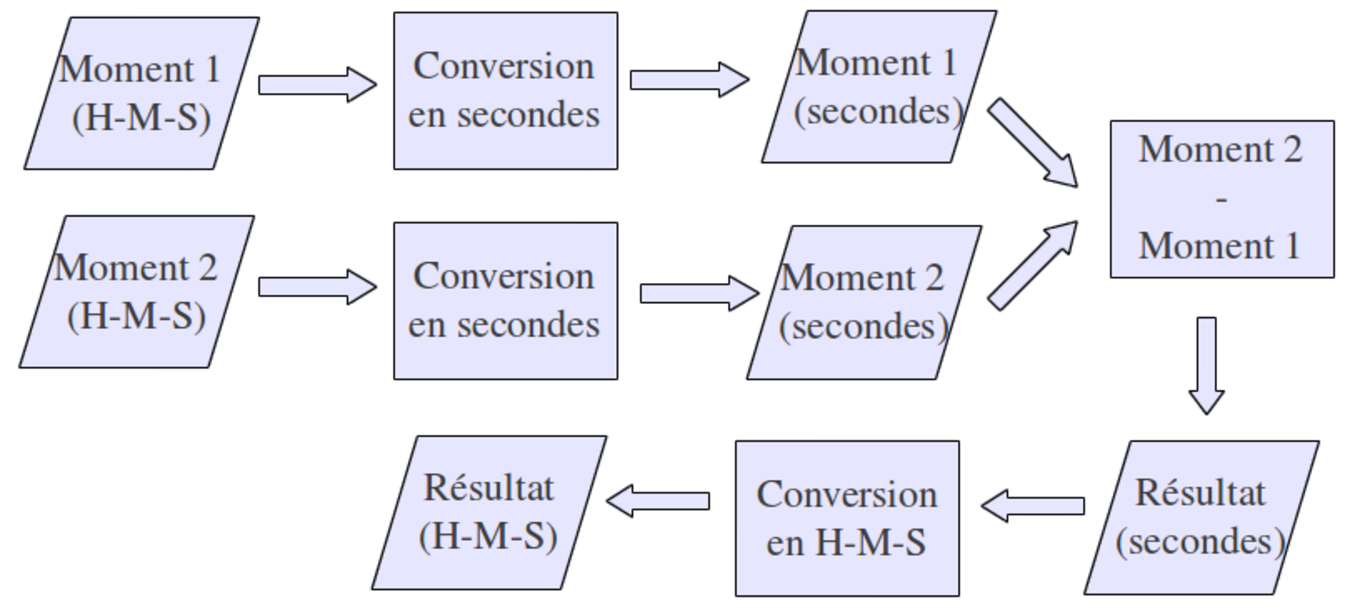
\includegraphics[width=0.8\textwidth]{image/module-conversion}
	\end{center}
\end{frame}

\subsubsection{Conversion en secondes}

\begin{frame}{Écart entre 2 moments}
	Une des sous-tâches est donc la conversion en secondes
	d'un moment exprimé en heures-minutes-secondes
	(h-m-s). 
	
	\bigskip
	
	Il nous faut adapter la solution trouvée pour
	l'exercice du chapitre sur les algorithmes séquentiels
	car il n'est pas question ici que les données soient
	lues ni que le résultat soit écrit~; 
	
	\bigskip
	
	l'interaction ne
	se fait pas avec l'utilisateur mais avec le module
	principal qui va l'utiliser.
\end{frame}

\begin{frame}{Écart entre 2 moments}
	La première question à se poser est donc celle des paramètres~:

	\bigskip
	
	\begin{itemize}
	\item 
		Quelles sont les données dont a besoin l'algorithme
		pour travailler ?
	\item 
		Quels résultats fournit-il ?
	\end{itemize}
\end{frame}

\begin{frame}{Écart entre 2 moments}
	Dans notre cas, la réponse est simple~:

	\bigskip
	
	\begin{itemize}
	\item {
		Les données sont le moment à convertir en secondes. 
		
		Ce moment est
		représenté par trois entiers~: les heures, les minutes et les secondes
		;}
	\item {
		Le résultat est le moment converti en secondes. 
		
		Il est représenté par un entier.}
	\end{itemize}
\end{frame}

\begin{frame}{Écart entre 2 moments}
	Lorsque le résultat est représenté par une seule donnée, on a le choix
	entre un paramètre en sortie~:

	\bigskip
	
	\cadre{
	\begin{pseudo}
		\LComment Affiche trois entiers~: des heures, des minutes et des secondes et sort le nombre de secondes correspondant.
		\ModuleSign{hmsVersSec}{h\In, m\In, s\In, secondes\Out~: entiers}{}
	\end{pseudo}
	}
	
	\bigskip
	
	ou une valeur de retour~:

	\bigskip
	
	\cadre{
	\begin{pseudo}
		\LComment Affiche trois entiers~: des heures, des minutes et des secondes et retourne le nombre de secondes correspondant.
		\ModuleSign{hmsVersSec}{h\In, m\In, s\In~: entiers}{entier}
	\end{pseudo}
	}
\end{frame}

\begin{frame}{Écart entre 2 moments}
		Dans de pareils cas, 
	on privilégie souvent la valeur de retour car cela
	facilite l'écriture lors de l'appel.

	\bigskip
	
	L'algorithme s'écrit alors~:

	\bigskip
	
	\cadre{
	\begin{pseudo}
	\LComment Affiche trois entiers~: des heures, des minutes et des secondes 
	\LComment et retourne le nombre de secondes correspondant.
		\Module{hmsVersSec}{h\In, m\In, s\In~: entiers}{entier}
			\Decl secondes~: entier \RComment {À déclarer puisque ce n'est pas un paramètre}
			\Let secondes \Gets  h * 3600 + m * 60 + s
			\Return secondes
		\EndModule
	\end{pseudo}
	}
\end{frame}

\begin{frame}{Écart entre 2 moments}
	ou de manière équivalente mais plus concise~:

	\bigskip
	
	\cadre{
	\begin{pseudo}
	\LComment Affiche trois entiers~: des heures, des minutes et des secondes 
	\LComment et retourne le nombre de secondes correspondant.
		\Module{hmsVersSec}{h\In, m\In, s\In~: entiers}{entier}
			\Return h * 3600 + m * 60 + s
		\EndModule
	\end{pseudo}
	}
\end{frame}

\subsubsection{Conversion en heures-minutes-secondes}

\begin{frame}{Conversion en heures-minutes-secondes}
	À la fin de notre algorithme, il nous faudra reconvertir un résultat
	exprimé en secondes sous la forme heures-minutes-secondes. 
	
	\bigskip
	
	À nouveau,
	on a déjà résolu ce problème dans le chapitre sur les algorithmes
	séquentiels. 
	
	\bigskip
	
	Mais il faut l'adapter à
	l'usage de paramètres.
\end{frame}

\begin{frame}{Conversion en heures-minutes-secondes}
	\begin{itemize}
	\item {
		Quelles sont les données ? 
		
		Une seule, le moment exprimé en secondes}
		
	\bigskip
	
	\item {
		Quels sont les résultats calculés par le module ? 
		
		Ce même moment exprimé
		en heures-minutes-secondes. 
		
		Trois entiers sont requis ce qui fait que
		le choix entre un paramètre en sortie et une valeur de retour ne se
		pose pas ici~; 
		
		impossible d'utiliser une valeur de
		retour (qui doit être unique)~; 
		
		on doit utiliser des paramètres en
		sortie.}
	\end{itemize}
\end{frame}

\begin{frame}{Conversion en heures-minutes-secondes}
	Ce qui donne~:

	\bigskip
	
	\cadre{
	\begin{pseudo}
		\LComment Affiche un nombre de secondes et sort les heures, les minutes et les secondes correspondant.
		\Module{secVersHMS}{secondes\In, s\Out, m\Out, s\Out~: entiers}{}
			\Let h \Gets secondes DIV 3600
			\Let m \Gets (secondes MOD 3600) DIV 60
			\Let s \Gets secondes MOD 60
		\EndModule
	\end{pseudo}
	}
\end{frame}

\subsubsection{Solution}

\begin{frame}{Solution}
	À présent, on a tout pour écrire la solution à notre problème

	\bigskip
	
	\cadre{
	\begin{pseudo}
		\LComment Lit deux moments (h-m-s) et affiche le moment de la différence entre les deux.
		\Module{différenceEntreHeures}{}{} \RComment Pas de paramètres !
			\Decl h1, m1, s1, h2, m2, s2~: entiers \RComment Les 2 moments à soustraire
			\Decl secondes1, secondes2~: entiers \RComment Ces 2 moments en secondes
			\Decl diffSecondes~: entier \RComment La différence en secondes
			\Decl diffH, diffM, diffS~: entiers \RComment La différence en H-M-S
			\Read h1, m1, s1, h2, m2, s2
			\Let secondes1 \Gets hmsVersSec( h1, m1, s1 )
			\Let secondes2 \Gets hmsVersSec( h2, m2, s2 )
			\Let diffSecondes \Gets secondes2 – secondes1
			\Stmt secVersHMS( diffSecondes, diffH, diffM, diffS )
			\Write diffH, diffM, diffS
		\EndModule
	\end{pseudo}
	}
\end{frame}

\begin{frame}{Solution}
	Dans la solution ci-dessus, 
	quelle est ou quelles sont la/les variable(s) locale(s) 
	dont on pourrait se passer moyennant une réécriture de
	l'algorithme ?
\end{frame}

\subsection{Blocs}

\begin{frame}{Blocs}
	\begin{itemize}
	\item
	Un bloc est l’écriture d’une portion de module
	à l’extérieur de celui-ci. C’est un simple
	{\textit{déplacement}}
	de lignes de codes vers un autre endroit du texte de
	l'algorithme.
	
	\bigskip
	
	\item
	La raison de découper un module en blocs
	peut être le souci de clarifier un algorithme en le découpant en étapes
	bien distinctes.
	
	\bigskip
	
	\item
	Les variables
	d’un bloc ne sont donc pas des variables locales du bloc dans lequel
	elles apparaissent, mais bien des variables locales du module auquel
	appartient ce bloc.
	\end{itemize}
\end{frame}

\begin{frame}{Blocs}
	\begin{itemize}
	\item
	L’appel de l’exécution des instructions se trouvant
	dans un bloc est similaire à celui d’un module avec paramètres, on
	écrit simplement le nom du bloc comme s’il s’agissait d’une
	instruction.
	\end{itemize}
\end{frame}

\begin{frame}{Blocs}
	Pour exemple, le module additionnerFractions (première version dans le
	chapitre 3) pourrait se découper ainsi~:

	\bigskip
	
	\cadre{
	\begin{pseudo}
	\LComment Lit les contenus de 2 fractions et affiche leur somme
		\Module{additionnerFractions}{}{}
			\Stmt déclaration
			\Stmt lectureDonnées
			\Stmt calculs
			\Stmt écritureRésultat
		\EndModule
	\end{pseudo}
	}
\end{frame}

\begin{frame}{Blocs}
	\cadre{
	\begin{pseudo}
	\Block{déclaration}
		\Decl num1, den1, num2, den2, numRes, denRes~: entiers
	\EndBlock
	\end{pseudo}
	}

	\bigskip
	
	\cadre{
	\begin{pseudo}
	\Block{lectureDonnées}
		\Read num1, den1, num2, den2
	\EndBlock
	\end{pseudo}
	}
\end{frame}

\begin{frame}{Blocs}
	\cadre{
	\begin{pseudo}
	\Block{calculs}
		\Let numRes \Gets num1 * den2 + num2 * den1
		\Let denRes \Gets den1 * den2
	\EndBlock
	\end{pseudo}
	}

	\bigskip
	
	\cadre{
	\begin{pseudo}
	\Block{écritureRésultat}
		\Write numRes, "/", denRes \RComment la fraction n'est pas simplifiée
	\EndBlock
	\end{pseudo}
	}
\end{frame}

\subsection{Qu'est-ce qu'un algorithme de qualité ?}

\begin{frame}{Algorithme de qualité}
	\begin{itemize}
	\item
	Nous voulons tous produire du code de qualité mais
	qu'est-ce que cette notion recouvre vraiment ?
	\item
	Qu'est-ce qui permet de juger de la qualité
	d'un code ? 
	\item
	De nombreux critères existent. 
	\end{itemize}
	
	\bigskip
	
	Citons ici,
	parmi les plus pertinents, ceux qui sont le plus liés à ce
	cours.
\end{frame}

\begin{frame}{Algorithme de qualité}
	\begin{itemize}
	\item
		La \textbf{validité}~: le code doit
	réaliser les tâches pour lesquelles 
	il a été écrit, même dans tous les
	cas particuliers imaginés.
	
	\bigskip
	
	\item 
		L'\textbf{extensibilité} (ou évolutivité)~:
	le code doit être écrit de telle sorte qu'un changement
	mineur dans le problème n'implique
	qu'un changement mineur dans le code.
	
	\bigskip
	
	\item
		La \textbf{réutilisabilité}~: c'est
	la capacité de réutiliser 
	un bout de code d’un projet dans un autre projet de 
	façon aisée et sûre.
	\end{itemize}
\end{frame}

\begin{frame}{Algorithme de qualité}
	\begin{itemize}
	\item
		La \textbf{lisibilité}~: 
		
	Au niveau global, on doit facilement comprendre la structure
	générale du code afin de pouvoir aisément comprendre où se trouve 
	la portion de	code qui nous intéresse. 
	
	Au niveau local, on doit pouvoir comprendre
	aisément chaque bout de code.
	
	\bigskip
	
	\item 
		L'\textbf{efficience}~: 
	ce critère s'intéresse à la bonne utilisation des
	ressources informatiques. Est-ce que le programme va tourner
	suffisamment vite, utiliser peu de mémoire ?
	\end{itemize}
\end{frame}

\section{Les variables structurées}
%\leconwithtoc

\subsection{Le type structuré}

\begin{frame}{types simple et structuré}
	\begin{itemize}
		\item
		Les variables de \code{types}
		dits «~\code{simples}~» ne peuvent
		contenir qu’une seule valeur à la fois  
		(entier, réel, booléen, caractère, chaine).
		
		\bigskip
	
		\item
		Cependant, certains types
		d’information consistent en un 
		regroupement de plusieurs données
		élémentaires.
		\begin{itemize}
			\item 
				une \textbf{date} est composée de trois éléments (le jour, le mois,
				l’année);
			\item {
				un \textbf{moment} de la journée est un triple d’entiers (heures,
				minutes, secondes)}
			\item {
				la localisation d’un \textbf{point} dans un plan nécessite 
				deux coordonnées cartésiennes (l’abscisse \textit{x} et
				l’ordonnée \textit{y}) ou polaires (le rayon \textit{r} et l’angle
				\textit{$\theta $})}
			\item {
				une \textbf{adresse }est composée de plusieurs données}
		\end{itemize}
		
	\end{itemize}
\end{frame}

\begin{frame}{type structuré}
	Pour stocker et manipuler de tels ensembles de données, nous utiliserons
	des \textbf{types structurés} ou \textbf{structures}.
	
	\bigskip
	
	\cadre{
	Une \code{structure} est donc un ensemble
	fini d’éléments pouvant être de types distincts. Chaque élément de cet
	ensemble, appelé \code{champ} de la structure, possède un nom unique.
	}
	
	\bigskip
	
	Noter qu’un champ d’une structure peut lui-même être une structure. 
	
	Par	exemple, une \textbf{carte d’identité} inclut parmi ses informations
	une \textbf{date} de naissance, l’\textbf{adresse} de son
	propriétaire (cachée dans la puce électronique!),\dots
\end{frame}

\subsection{Définition d'une structure}

\begin{frame}{Définition}
	La définition d’un type structuré adoptera le modèle suivant~:

	\bigskip
	
	\cadre{
	\begin{pseudo}
	\Struct{NomDeLaStructure}
		\Decl nomChamp1~: type1
		\Decl nomChamp2~: type2
		\Decl \dots
		\Decl nomChampN~: typeN
	\EndStruct
	\end{pseudo}
	}

	\bigskip
	
	\textit{nomChamp1}, \dots, \textit{nomChampN }
	sont les noms des différents champs de la structure, 
	et \textit{type1}, \dots, \textit{typeN} 
	les types de ces champs. 
	
	\bigskip
	
	Ces types sont 
	\begin{itemize}
	\item
	soit les types «~simples~» étudiés
	précédemment (entier, réel, booléen, caractère, chaine) 
	\item
	soit d’autres
	types structurés dont la structure aura été préalablement définie.
	\end{itemize}
\end{frame}

\begin{frame}{Exemple}
	Pour exemple, nous définissons ci-dessous trois
	types structurés que nous utiliserons souvent par la suite~:

	\bigskip
	
	\cadre{
	\begin{pseudo}
	\Struct{Date}
		\Decl jour~: entier
		\Decl mois~: entier
		\Decl année~: entier
	\EndStruct
	\end{pseudo}
	}
\end{frame}

\begin{frame}{Exemple}
	\cadre{
	\begin{pseudo}
	\Struct{Moment}
		\Decl heure~: entier
		\Decl minute~: entier
		\Decl seconde~: entier
	\EndStruct
	\end{pseudo}
	}

	\bigskip
	
	\cadre{
	\begin{pseudo}
	\Struct{Point}
		\Decl x~: réel
		\Decl y~: réel
	\EndStruct
	\end{pseudo}
	}

\end{frame}

\subsection{Déclaration d’une variable de type structuré}

\begin{frame}{Exemple}
	Une fois un type structuré défini, la
	déclaration de variables de ce type est identique à celle des variables
	simples. 
	
	\bigskip
	
	Par exemple~:

	\bigskip
	
	\cadre{
	\begin{pseudo}
	\Decl anniversaire, jourJ~: Date
	\Decl départ, arrivée, unMoment~: Moment
	\Decl a, b, centreGravité~: Point
	\end{pseudo}
	}
\end{frame}

\subsection{Utilisation des variables de type structuré}

\begin{frame}{Utilisation d'un champ}
	Pour accéder à l’un des champs d’une variable structurée, il faut mentionner
	le nom de ce champ ainsi que celui de la variable dont il fait partie.
	
	\bigskip
	
	Nous utiliserons la notation «~pointée~»~:
	
	\bigskip

	\cadre{
	\begin{pseudo}
	\Stmt nomVariable.nomChamp
	\end{pseudo}
	}
\end{frame}

\begin{frame}{Exemple}	
	\cadre{
	\begin{pseudo}
	\Let anniversaire.jour \Gets 15
	\Let anniversaire.mois \Gets 10
	\Let anniversaire.année \Gets 2014
	\Let arrivée.heure \Gets départ.heure + 2
	\Let centreGravité.x \Gets (a.x + b.x) / 2
	\end{pseudo}
	}
\end{frame}

\begin{frame}{Utilisation globale}
		On peut cependant, dans certains cas, utiliser
	une variable structurée de manière globale (c’est-à-dire d’une façon
	qui agit simultanément sur chacun de ses champs). 
	
	\bigskip
	
	Le cas le plus
	courant est l’affectation interne entre deux variables structurées de
	même type, par exemple~:

	\bigskip
	
	\cadre{
	\begin{pseudo}
	\Let arrivée \Gets départ
	\end{pseudo}
	}

	\bigskip
	
	qui résume les trois instructions suivantes~:

	\bigskip
	
	\cadre{
	\begin{pseudo}
	\Let arrivée.heure \Gets départ.heure
	\Let arrivée.minute \Gets départ.minute
	\Let arrivée.seconde \Gets départ.seconde
	\end{pseudo}
	}
\end{frame}

\begin{frame}{Paramètre d'un module}
	Une variable structurée peut aussi être le
	paramètre d’un module, et un module peut également renvoyer une
	«~valeur~» de type structuré. 
	
	\bigskip
	
	Par exemple, l’entête d’un module
	renvoyant le nombre de secondes écoulées entre une heure de départ et
	d’arrivée serait~:

	\bigskip
	
	\cadre{
	\begin{pseudo}
	\ModuleSign{nbSecondesEcoulées}{ départ\In, arrivée\In~: Moment}{entier}
	\end{pseudo}
	}
\end{frame}

\begin{frame}{Lire et afficher}
	On pourra aussi lire ou afficher une variable structurée.

	\bigskip
	
	\cadre{
	\begin{pseudo}
	\Read unMoment
	\Write unMoment
	\end{pseudo}
	}
\end{frame}

\begin{frame}{Comparaison}
	On ne peut pas utiliser les opérateurs de comparaison ({\textless}, {\textgreater}) pour
	comparer des variables structurées. 
	
	\bigskip
	
	En effet, s’il est naturel de vouloir comparer des dates ou des moments,
	comment définir une relation d’ordre avec les points du plan ou avec
	des cartes d’identités ?

	\bigskip
	
	Si le besoin de comparer des variables
	structurées se fait sentir, il faudra dans ce cas écrire des modules de
	comparaison adaptés aux structures utilisées.
\end{frame}

\begin{frame}{Assignation globale}
	Par facilité d'écriture, on peut assigner tous les champs en une 
	fois via des «~\{\}~». 
	
	\bigskip
	
	Exemple~:

	\bigskip
	
	\cadre{
	\begin{pseudo}
	\Let anniversaire \Gets \{1, 9, 1989\}
	\end{pseudo}
	}
\end{frame}

\subsection{Exemple d’algorithme}

\begin{frame}{Exemple}	
	Le module ci-dessous reçoit en paramètre deux dates ; 
	
	la valeur renvoyée est 
	\begin{itemize}
	\item
	–1 si la première date est antérieure à la deuxième, 
	\item
	0 si les deux	dates sont identiques 
	\item
	1 si la première date est postérieure à la
	deuxième.
	\end{itemize}
\end{frame}

\begin{frame}{Exemple}	
		\cadre{
	\begin{pseudo}
	\Module{comparerDates}{date1\In, date2\In~: Date}{entier}
		\Decl résultat~: entier
		\Let  résultat \Gets -1
		\RComment valeur choisie par défaut
		\If{date1.année ${\geq}$ date2.année}
			\If{date1.année $>$ date2.année}
				\Let  résultat \Gets 1
			\Else \RComment les années sont identiques
				\If{date1.mois ${\geq}$ date2.mois}
					\If{date1.mois $>$ date2.mois}
						\Let  résultat \Gets 1
					\Else \RComment les années et les mois sont identiques
						\If{date1.jour ${\geq}$ date2.jour}
							\If{date1.jour $>$ date2.jour}
								\Let  résultat \Gets 1
							\Else \RComment les années, les mois et les jours sont identiques
								\Let  résultat \Gets 0
							\EndIf
						\EndIf
					\EndIf
				\EndIf
			\EndIf
		\EndIf
		\Return résultat
	\EndModule
	\end{pseudo}
	}
\end{frame}

\section{Les boucles}
%\leconwithtoc

\subsection{La notion de travail répétitif}

\begin{frame}{La notion de travail répétitif}
	\begin{itemize}
		\item
		Les ordinateurs révèlent tout leur potentiel dans leur capacité à
		répéter inlassablement les mêmes tâches. 
	\item
		Si on veut faire effectuer un travail répétitif, 
		il faut indiquer deux choses~:
		
		\begin{enumerate}
			\item Le travail à répéter
			\item La manière de continuer la répétition 
				ou de l'arrêter.
		\end{enumerate}

	\end{itemize}
\end{frame}

\begin{frame}{Exemple 1}
	Pour traiter des dossiers, on dira quelque chose
	comme «~tant qu'il reste un dossier à traiter, le
	traiter~» ou encore «~traiter un dossier puis passer au suivant
	jusqu'à ce qu'il n'en reste plus à traiter~».

	\begin{itemize}
	\item la tâche à répéter est : «~traiter un dossier~»
	\item on indique qu'on doit continuer s'il
		reste encore un dossier à traiter
	\end{itemize}
	
	\bigskip

	\textbf{Remarque :} On aurait aussi pu le formuler ainsi : «~traiter un
	dossier et passer au suivant jusqu'à ce
	qu'il n'en reste plus~»
\end{frame}

\begin{frame}{Exemple 2}
	Pour calculer la cote finale de tous les étudiants,
	on aura quelque chose du genre «~Pour tout étudiant, calculer sa
	cote~»

	\begin{itemize}
	\item 
		La tâche à répéter est : «~calculer la cote d'un
		étudiant~»
	\item 
		On indique qu'on doit le faire pour tous les étudiants.
		On doit donc commencer par le premier, passer à chaque fois au suivant
		et s'arrêter quand on a fini le dernier.
	\end{itemize}
\end{frame}

\begin{frame}{Exemple 3}
	Pour afficher tous les nombres de 1 à 100, on aura
	«~Pour tous les nombres de 1 à 100, afficher ce nombre~»

	\begin{itemize}
	\item
		La tâche à répéter est : «~afficher un nombre~»
	\item 
		On indique qu'on doit le faire pour tous les nombres de
		1 à 100. On doit donc commencer avec 1, passer à chaque fois au nombre
		suivant et s'arrêter après avoir affiché le nombre
		100.
	\end{itemize}
\end{frame}

\begin{frame}{Attention}
	\textbf{Attention} ! Comprenez bien que c'est toujours
	la même tâche qui est exécutée mais pas avec le même effet à chaque
	fois. Ainsi, on traite un dossier mais à chaque fois un différent; on
	affiche un nombre mais à chaque fois un différent. 
	
	Voyons comment	y arriver en logique.
\end{frame}

\subsection{Structures itératives}

\subsubsection{«~tant que~»}

\begin{frame}{Tant que}
	Le «~tant que~» est une structure qui demande à
	l'exécutant de répéter une tâche (une ou plusieurs
	instructions) tant qu'une condition donnée est vraie.

	\bigskip

	\cadre{
		\begin{pseudo}
		\While{condition}
			\Stmt séquence d’instructions à exécuter
		\EndWhile
		\end{pseudo}
	}

\end{frame}

\begin{frame}{Tant que}
	\begin{itemize}
		\item
			Comme pour la structure \code{si}, la \code{condition} est
			une expression à valeur booléenne.
		\item
			Dans ce type de structure, il faut
			qu’il y ait dans la séquence d’instructions comprise entre
			\code{tant que} et \code{fin tant que} au moins une
			instruction qui modifie une des composantes de la condition de telle
			manière qu’elle puisse devenir \textbf{fausse} à un moment donné.
		\item 
			Dans le cas contraire, la condition reste indéfiniment vraie et la boucle va
			tourner sans fin, c'est ce qu'on appelle une \textbf{boucle infinie}.
		\item
			Si la condition est fausse dès le début, 
			la tâche n'est jamais exécutée.
	\end{itemize}
\end{frame}

\begin{frame}{Tant que}
	\begin{figure}[h]
		\centering
		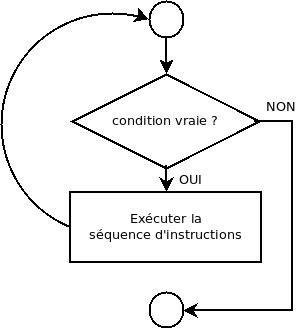
\includegraphics[width=0.5\textwidth]{image/boucle-tq}
		\caption{Ordinogramme de la boucle "tant-que"}
		\label{fig:boucle-tq}
	\end{figure}
\end{frame}

\subsubsection{«~faire – jusqu'à ce que~»}

\begin{frame}{«~faire – jusqu'à ce que~»}
	Cette structure est très proche du «~tant que~» 
	à deux différences près :
	
	\begin{enumerate}
		\item {
			Le test est fait à la fin et pas au début. La tâche est donc toujours
			exécutée au moins une fois. }
		\item {
			On donne la condition pour arrêter et pas pour continuer; il
			s'agit d'une différence mineure.}
	\end{enumerate}

	\bigskip
	
	\cadre{
		\begin{pseudo}
		\Repeat
			\Stmt séquence d’instructions à exécuter
		\Until{condition}
		\end{pseudo}
	}
\end{frame}

\begin{frame}{«~faire – jusqu'à ce que~»}
	\begin{itemize}
		\item 
			la séquence d’instructions comprise entre
			\code{faire} et \code{jusqu'a ce que} 
			contienne au moins une instruction qui modifie la condition de
			telle manière qu’elle puisse devenir \textbf{vraie} à un moment donné
			pour arrêter l'itération. 
	\end{itemize}
\end{frame}

\begin{frame}{«~faire – jusqu'à ce que~»}
	\begin{figure}[h]
	\centering
	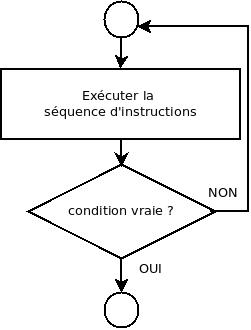
\includegraphics[width=0.4\textwidth]{image/boucle-faire}
	\caption{Ordinogramme de la boucle "faire – jusqu'à ce que"}
	\label{fig:boucle-faire}
	\end{figure}
\end{frame}

\subsubsection{«~pour~»}

\begin{frame}{«~pour~»}
	\begin{itemize}
		\item
		Ici, on va plutôt indiquer \textbf{combien de fois} la tâche doit être
		répétée. 
		\item
		Cela se fait au travers d'une
		\textbf{variable de contrôle} dont la valeur va évoluer à partir
		d'une valeur de départ jusqu'à une
		valeur finale.
	\end{itemize}
\end{frame}

\begin{frame}{«~pour~»}
	\cadre{
		\begin{pseudo}
		\For{variable \K{de} début \K{à} fin [\K{par} pas]}
			\Stmt séquence d’instructions à exécuter
		\EndFor
		\end{pseudo}
	}

	\begin{itemize}
		\item
		Dans ce type de structure, \code{debut}, \code{fin} et \code{pas}
		peuvent être des constantes, des variables ou des expressions (le plus
		souvent à valeurs entières mais on admettra parfois des réels). 
		\item
		Le \code{pas} est facultatif, et généralement omis (dans ce cas, sa valeur 
		par défaut est 1). 
		\item
		Ce pas est parfois négatif, dans le cas
		d'un compte à rebours, par exemple
		\code{pour n de 10 a 1 par -1}.
	\end{itemize}
\end{frame}

\begin{frame}{«~pour~»}
	\begin{itemize}
		\item
		Quand le \code{pas} est positif, la boucle s'arrête
		lorsque la variable dépasse la valeur de \code{fin}.
		\item
		Par contre, avec
		un \code{pas} négatif, la boucle s'arrête lorsque la
		variable prend une valeur plus petite que la valeur de \code{fin}
	\end{itemize}
\end{frame}

\begin{frame}{«~pour~»}
	\begin{figure}[h]
		\centering
		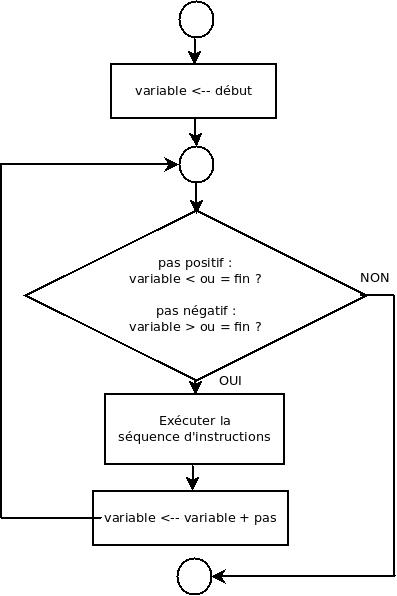
\includegraphics[width=0.4\textwidth]{image/boucle-pour}
		\caption{Ordinogramme de la boucle "pour"}
		\label{fig:boucle-pour}
		\end{figure}
\end{frame}

\begin{frame}{Attention}
	\begin{itemize}
		\item
		On considérera
		qu’au cas (à éviter) où \code{debut} est strictement supérieur à
		\code{fin} et le \code{pas} est positif, la séquence d’instructions
		n’est jamais exécutée (mais ce n’est pas le cas dans tous les langages
		de programmation !). 
		\item
		Idem si \code{debut} est strictement inférieur à
		\code{fin} mais avec un \code{pas} négatif.
		\item
		Attention de ne pas modifier dans la séquence d’instructions une des
		variables de contrôle \code{debut}, \code{fin} ou \code{pas} !
	\end{itemize}
\end{frame}

\begin{frame}{Attention}
	\begin{itemize}
		\item
		Il est aussi fortement déconseillé de modifier «~manuellement~» la
		\code{variable} de contrôle au sein de la boucle
		\code{pour}. Il ne faut pas l’initialiser en début de boucle,
		et ne pas s’occuper de sa modification, l’instruction 
		\code{variable} $\leftarrow$ \code{variable} + \code{pas} 
		étant automatique et implicite à chaque étape de la
		boucle.
		\item
		Il est aussi déconseillé d’utiliser \code{variable} à la
		sortie de la structure \code{pour} sans lui affecter une
		nouvelle valeur (son contenu pouvant varier selon le langage de
		programmation).
	\end{itemize}
\end{frame}


\begin{frame}{Exemples~}
	\cadre{
	\begin{pseudo}
	\Stmt \K{pour} i \K{de} 0 \K{à} 2 \K{faire} \RComment La boucle est exécutée 3 fois.
	\Stmt \K{pour} i \K{de} 2 \K{à} 0 \K{faire} \RComment La boucle n'est pas exécutée.
	\Stmt \K{pour} i \K{de} 1 \K{à} 10 \K{par} -1 \K{faire} \RComment La boucle n'est pas exécutée.
	\Stmt \K{pour} i \K{de} 1 \K{à} 1 \K{par} 5 \K{faire} \RComment La boucle est exécutée 1 fois.
	\end{pseudo}
	}
\end{frame}	

\subsection{Quel type de boucle choisir ?}

\begin{frame}{Quelle boucle choisir ?}
	\begin{itemize}
		\item
		En pratique, il est possible d’utiliser systématiquement la boucle 
		\code{tant que} qui peut s’adapter à toutes les situations. 
		\item
		Cependant, il est plus clair d’utiliser la boucle \code{pour} 
		dans les cas où le nombre d’itérations est fixé et connu à l’avance 
		\item
		La boucle \code{faire} convient quant à elle
		dans les cas où le contenu de la boucle doit être parcouru au moins une
		fois, 
		
		alors que dans \code{tant que}, 
		le nombre de parcours peut être nul si la condition initiale est fausse. 
	\end{itemize}
\end{frame}

\begin{frame}{Quelle boucle choisir ?}
	\begin{figure}[h]
	\centering
	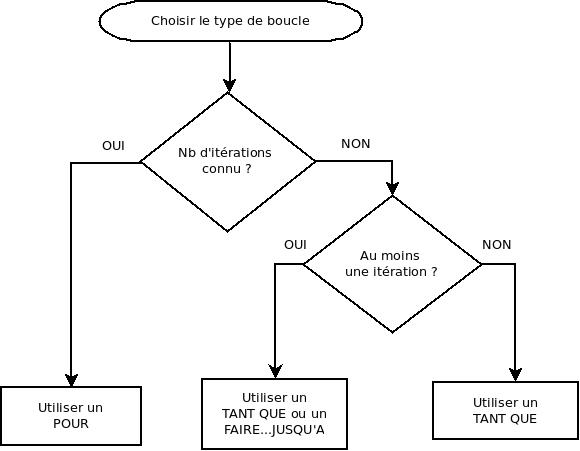
\includegraphics[width=0.7\textwidth]{image/boucle-choixtype}
	\caption{Quel type de boucle choisir ?}
	\label{fig:boucle-choix}
	\end{figure}
\end{frame}
	
\subsection{Exemples}

\subsubsection{Exemple 1 -- Compter de 1 à 10}

\begin{frame}{Compter de 1 à 10}
	Imaginons qu'on veuille afficher tous les nombres de 1 à 10. 
	
	On va évidemment \textbf{rejeter} cette première solution :

	\cadre{
	\begin{pseudo}
	\LComment Affiche les nombres de 1 à 10.
	\Module{compterJusque10}{}{} \RComment une mauvaise solution !
	\Write 1
	\Write 2
	\Write 3
	\Write 4
	\Write 5
	\Write 6
	\Write 7
	\Write 8
	\Write 9
	\Write 10
	\EndModule
	\end{pseudo}
	}
\end{frame}

\begin{frame}{Compter de 1 à 10}
	\begin{itemize}
	\item
	Non seulement c'est long à écrire 
	(imaginer l'algorithme pour afficher les nombres de 1 à 10000 !) 
	mais c'est très peu souple.
	\item
	Cela ne fonctionne que pour 10 : il faut modifier l'algorithme pour
	un autre comptage.
	\item
	La boucle va nous permettre
	d'obtenir un algorithme qui s'adapte
	à la limite du décompte.
	\end{itemize}
\end{frame}
	
\begin{frame}{Compter de 1 à 10}
	Posons-nous les bonnes questions pour déterminer la boucle :

	\begin{itemize}
	\item 
		Quelle est la tâche à répéter ? Afficher un nombre.
	\item 
		Comment savoir si on continue ? On arrête quand «~10~» est affiché.
	\item 
		Comment afficher à chaque fois un nombre différent ? 
		Au travers d'une variable qui prendra toutes les valeurs de 1 à 10. 
		Il faut donc ajouter dans le corps de la
		boucle une incrémentation de la variable
	\end{itemize}
\end{frame}

\begin{frame}{Compter de 1 à 10}
	Ce qui donne :

	\cadre{
	\begin{pseudo}
	\LComment A les nombres de 1 à 10.
	\Module{compterJusque10}{}{} \RComment version avec tant que
		\Decl nb : entier
		\Let nb \Gets 1 \RComment c'est le premier nombre à afficher
		\While{nb $\leq$ 10} \RComment tant que le nb à afficher est toujours bon
			\Write nb \RComment on affiche la valeur de la variable nb
			\Let nb \Gets nb + 1 \RComment on passe au nombre suivant
		\EndWhile
	\EndModule
	\end{pseudo}
	}
\end{frame}

\begin{frame}{Compter de 1 à 10}
	Mais ici, on pourrait aussi l'écrire avec un «~pour~» vu qu'on
	connait exactement le nombre d'exécutions de la boucle (10). 
	
	\medskip
	
	La variable de contrôle va évoluer de 1 à 10 ce qui tombe bien car
	c'est justement le nombre à afficher à chaque fois.
	
	\medskip

	\cadre{
	\begin{pseudo}
	\LComment Affiche les nombres de 1 à 10.
	\Module{compterJusque10}{}{} \RComment version avec pour
		\Decl nb : entier
		\For{nb \K{de} 1 \K{à} 10} \RComment par défaut le pas est de 1
			\Write nb 
		\EndFor
	\EndModule
	\end{pseudo}
	}
\end{frame}

\subsubsection{Exemple 2 -- Compter de 1 à beaucoup}

\begin{frame}{Compter de 1 à beaucoup}
	Dans l'exercice précédent, on a
	affirmé que la boucle pouvait s'adapter à la limite du
	décompte. Montrons-le ! 
	
	\bigskip
	
	Supposons qu'on veuille
	afficher les nombres de 1 à $n$ où $n$ est une valeur 
	donnée par l'utilisateur.

	\bigskip

	Rien de plus simple, il suffit de lire cette
	valeur au début et de l'utiliser comme limite de boucle
\end{frame}

\begin{frame}{Compter de 1 à beaucoup}
	\cadre{
	\begin{pseudo}
	\LComment Lit un nombre et affiche les nombres de 1 à ce nombre.
	\Module{afficherN}{}{} 
		\Decl nb, n : entier
		\Read n
		\For{nb \K{de} 1 \K{à} n} 
			\Write nb 
		\EndFor
	\EndModule
	\end{pseudo}
	}
\end{frame}

\begin{frame}{Compter de 1 à beaucoup}
	Que se passe-t-il si l'utilisateur entre une valeur négative ?
	
	\bigskip
	
	Comment améliorer le code pour que le programme
	le signale à l'utilisateur ?
\end{frame}

\subsubsection{Exemple 3 -- Afficher les nombres pairs}

\begin{frame}{Afficher les nombres pairs}
	Cette fois-ci on affiche uniquement les nombres 
	\textbf{pairs} jusqu'à la limite $n$.
	
	\bigskip
	
	\textbf{Exemple} : 
	les nombres pairs de $1$ à $10$ sont : $2$, $4$, $6$, $8$, $10$.
	
	\bigskip
	
	Notez que $n$ peut être impair. Si $n$ vaut $11$, 
	l'affichage est le même que pour $10$.

	\bigskip

	Est-ce qu'on peut utiliser un «~pour~» ? 
\end{frame}

\begin{frame}{Afficher les nombres pairs}
	Est-ce qu'on peut utiliser un «~pour~» ? 

	\bigskip
	
	Oui. De 1 à $n$, il y a exactement «~$n$ DIV $2$~» nombres à afficher. 
	
	\bigskip
	
	La difficulté vient du lien à faire entre la variable de
	contrôle et le nombre à afficher.
\end{frame}

\begin{frame}{Afficher les nombres pairs}

	\textbf{Solution 1} : 
	on garde le lien entre la variable de contrôle 
	et le nombre à afficher. 
	Dans ce cas, on commence à $2$ et le pas doit être de $2$.

	\bigskip
	
	\cadre{
	\begin{pseudo}
	\LComment Lit un nombre et affiche les nombres pairs jusqu'à ce nombre.
	\Module{afficherPair}{}{} 
		\Decl nb, n : entier
		\Read n
		\RComment limite des nombres à afficher
		\For{nb \K{de} 2 \K{à} n \K{par} 2} 
			\Write nb 
		\EndFor
	\EndModule
	\end{pseudo}
	}
\end{frame}

\begin{frame}{Afficher les nombres pairs}
	\textbf{Solution 2} : 
	la variable de contrôle compte simplement le nombre d'itérations.
	
	Alors il faut calculer le nombre à afficher en fonction de la variable
	de contrôle (ici le double de celle-ci convient)

	\bigskip
	
	\cadre{
	\begin{pseudo}
	\LComment Lit un nombre et affiche les nombres pairs jusqu'à ce nombre.
	\Module{afficherPair}{}{} 
		\Decl i, n : entier
		\Read n
		\RComment limite des nombres à afficher
		\For{i \K{de} 1 \K{à} n DIV 2} 
			\Write 2 * i 
		\EndFor
	\EndModule
	\end{pseudo}
	}
\end{frame}

\subsection{Exemple 4 -- Afficher les premiers nombres pairs}

\begin{frame}{Afficher les premiers nombres pairs}
	Voici un problème proche du précédent : 
	on affiche cette fois les $n$ premiers nombres pairs.
	
	\bigskip
	
	\textbf{Exemple} : 
	les $10$ premiers nombres pairs sont : $2$, $4$, $6$, $8$, $10$, $12$, $14$, $16$, $18$, $20$.
	
	\bigskip
	
	Il est plus simple de partir de la solution 2 de l'exemple précédent
	en changeant simplement la valeur finale de la boucle.
\end{frame}

\begin{frame}{Afficher les premiers nombres pairs}

		\cadre{
		\begin{pseudo}
		\LComment Lit un nombre et affiche ce nombre de nombres pairs.
		\Module{afficherPair}{}{} 
			\Decl i, n : entier
			\Read n
			\RComment le nombre de nombres à afficher
			\For{i \K{de} 1 \K{à} n} 
				\Write 2 * i 
			\EndFor
		\EndModule
		\end{pseudo}
		}
\end{frame}

\subsubsection{Exemple 5 -- Somme de nombres}

\begin{frame}{Somme de nombres}
	On veut pouvoir calculer (et retourner)
	la somme d'une série de nombres donnés par
	l'utilisateur. 
	
	\bigskip
	
	Il faut d'abord se
	demander comment l'utilisateur va pouvoir indiquer
	combien de nombres il faut additionner ou quand est-ce que le dernier
	nombre à additionner a été entré. 
	
	\bigskip
	
	Voyons quelques possibilités.
\end{frame}

\begin{frame}{Somme de nombres}
	\textbf{Variante 1}~: 
	
	L'utilisateur indique le nombre de termes au départ.
	
	\cadre{
	\begin{pseudo}
	\LComment Lit des valeurs entières et retourne la somme des valeurs lues.
	\Module{sommeNombres}{}{entier} \RComment Variante 1
		\Decl nbValeurs : entier \RComment nb de valeurs à additionner
		\Decl valeur : entier \RComment un des termes de l'addition
		\Decl somme : entier \RComment la somme
		\Decl i : entier \RComment itérateur
		\Let somme \Gets 0 \RComment la somme se construit petit à petit. 0 au départ
		\Read nbValeurs
		\For{i \K{de} 1 \K{à} nbValeurs} 
			\Read valeur
			\Let somme \Gets somme + valeur 
		\EndFor
		\Return somme
	\EndModule
	\end{pseudo}
	}
\end{frame}

\begin{frame}{Somme de nombres}
	\textbf{Variante 2}~: 
		
	Après chaque nombre, 
	on demande à l'utilisateur s'il y a encore un nombre à additionner.

	\bigskip
	
	Ici, il faut chercher une solution différente
	car on ne connait pas au départ le nombre de valeurs à additionner et
	donc le nombre d'exécution de la boucle. 
	
	\bigskip
	
	On va devoir passer à un
	«~tant que~» ou un «faire - jusqu'à ce que». 
	
	\bigskip
	
	On peut
	envisager de demander en fin de boucle si il reste
	encore un nombre à additionner. 
\end{frame}

\begin{frame}{Somme de nombres}
	\cadre{
	\begin{pseudo}
	\LComment Lit des valeurs entières et retourne la somme des valeurs lues.
	\Module{sommeNombres}{}{entier} \RComment Variante 2a
		\Decl encore : booléen \RComment est-ce qu'il reste encore une valeur à additionner ?
		\Decl valeur : entier \RComment un des termes de l'addition
		\Decl somme : entier \RComment la somme
		\Let somme \Gets 0
		\Repeat 
			\Read valeur
			\Let somme \Gets somme + valeur 
			\Read encore
		\Until{NON encore}
		\Return somme
	\EndModule
	\end{pseudo}
	}
\end{frame}

\begin{frame}{Somme de nombres}
	Avec cette solution, on additionne au moins une valeur. 
	
	\bigskip
	
	Si on veut pouvoir tenir compte du
	cas très particulier où l'utilisateur ne veut
	additionner aucune valeur, il faut utiliser un «~tant que~» et donc
	poser la question avant d'entrer dans la boucle.
\end{frame}

\begin{frame}{Somme de nombres}
	\cadre{
	\begin{pseudo}
	\LComment Lit des valeurs entières et retourne la somme des valeurs lues.
	\Module{sommeNombres}{}{entier} \RComment Variante 2b
		\Decl encore : booléen \RComment est-ce qu'il reste encore une valeur à additionner ?
		\Decl valeur : entier \RComment un des termes de l'addition
		\Decl somme : entier \RComment la somme
		\Let somme \Gets 0
		\Read encore
		\While{encore} 
			\Read valeur
			\Let somme \Gets somme + valeur 
			\Read encore
		\EndWhile
		\Return somme
	\EndModule
	\end{pseudo}
	}
\end{frame}

\begin{frame}{Somme de nombres}
	\textbf{Variante 3}~:
	
	L'utilisateur entre une valeur spéciale pour indiquer la fin. 
	On parle de valeur \textbf{sentinelle}. 
	
	\bigskip
	
	Ceci n'est possible que si cette valeur \textbf{sentinelle} ne peut pas être
	un terme valide de l'addition. 
	
	\bigskip
	
	Par exemple, si on veut
	additionner des nombres positifs uniquement, la valeur -1 peut servir
	de valeur sentinelle. 
	
	\bigskip
	
	Mais sans limite sur les nombres à additionner
	(positifs, négatifs ou nuls) il n'est pas possible de
	choisir une sentinelle.
\end{frame}

\begin{frame}{Somme de nombres}
	Ici, on se base sur la valeur entrée pour décider si on continue ou pas. 
	
	\bigskip
	
	Il faut donc \textbf{toujours} effectuer un test
	après une lecture de valeur. 
	
	\bigskip
	
	C'est pour cela
	qu'il faut effectuer une lecture avant et une autre à
	la fin de la boucle.

\end{frame}

\begin{frame}{Somme de nombres}
	\cadre{
	\begin{pseudo}
	\LComment Lit des valeurs entières et retourne la somme des valeurs lues.
	\Module{sommeNombres}{}{entier} \RComment Variante 3
		\Decl valeur : entier \RComment un des termes de l'addition
		\Decl somme : entier \RComment la somme
		\Let somme \Gets 0
		\Read valeur
		\While{valeur ${\geq}$ 0} 
			\Let somme \Gets somme + valeur 
			\Read valeur \RComment remarquer l'endroit où on lit une valeur.
		\EndWhile
		\Return somme
	\EndModule
	\end{pseudo}
	}
\end{frame}

\begin{frame}{Somme de nombres}
	\textbf{Réflexions}~: 
	\begin{itemize}
	\item
		Quelle valeur sentinelle prendrait-on 
		pour additionner une série de cotes d'interrogations ? 
		Une série de températures ?
	\item
		Dans les solutions 2 et 3 on lit une variable booléenne. 
		Comment un programmeur pourrait-il réaliser 
		cette instruction de façon pratique ?		
	\end{itemize}
\end{frame}

\subsubsection{Exemple 6~: Suite des nombres pairs}

\begin{frame}{Suite des nombres pairs}
	Écrire l'algorithme qui affiche les $n$ premiers termes
	de la suite: $2$, $4$, $6$\dots
	
	\bigskip
	
	Puisqu'on doit écrire plusieurs nombres et qu'on sait exactement combien,
	on se tournera tout naturellement vers une boucle \K{pour}.

	\bigskip
	
	Le cas le plus simple est lorsque le nombre à afficher à l'étape $i$
	peut être calculé en fonction de $i$ seulement.
	
\end{frame}

\begin{frame}{Suite des nombres pairs}
	\cadre{
	\begin{pseudo}
	\For{i de 1 à n}
		\Write $f(i)$
	\EndFor
	\end{pseudo}
	}
\end{frame}

\begin{frame}{Suite des nombres pairs}

	Dans ce cas, la fonction est $f(i)=2*i$
	(Si vous n'êtes pas convaincu, vérifiez qu'à l'étape $1$ on affiche $2$,
	à l'étape $2$ on affiche $4$ \dots)
	
	\bigskip

	\cadre{
	\begin{pseudo}
	\Module{nombrePair}{n\In: entier}{}
		\Decl i : entier
		\For{i de 1 à n}
			\Write 2 * i
		\EndFor
	\EndModule
	\end{pseudo}
	}
\end{frame}

\begin{frame}{Suite des nombres pairs}
	Parfois, il est difficile (voire impossible) de trouver $f(i)$.
	
	\bigskip
	
	On suivra alors une autre approche qui revient à calculer un nombre
	à afficher à partir du nombre précédemment affiché
	(ou, plus exactement, de calculer le suivant à partir du nombre
	qu'on vient d'afficher).
	La structure générale est alors

	\bigskip
	
	\cadre{
	\begin{pseudo}
	\Let nb \Gets \textit{\{1\up{ère} valeur à afficher\}}
	\For{i de 1 à n}
		\Write nb
		\Let nb \Gets \textit{\{calculer ici le nb suivant\}}
	\EndFor
	\end{pseudo}
	}
\end{frame}

\begin{frame}{Suite des nombres pairs}
	Dans l'exemple de la suite paire, le 1\up{er} nombre à afficher est $2$
	et le nombre suivant se calcule en ajoutant $2$ au nombre courant.

	\bigskip
	
	\cadre{
	\begin{pseudo}
	\Module{suite1}{n\In: entier}{}
		\Decl nb, i : entiers
		\Let nb \Gets 2
		\For{i de 1 à n}
			\Write nb
			\Let nb \Gets nb + 2
		\EndFor
	\EndModule
	\end{pseudo}
	}
\end{frame}

\begin{frame}{Suite des nombres pairs}
	On remarque que, lors du dernier passage dans la boucle,
	on calcule une valeur qui ne sera pas affichée.
	Cette petite perte de temps est dommage mais négligeable
	et permet de garder une structure claire et générale à la solution.

	\bigskip
	
	Dans certains cas,
	il n'est pas possible de déduire directement le nombre suivant
	en connaissant juste le nombre précédent.
	Prenons un exemple pour l'illustrer.
\end{frame}

\subsection{Exemple 7~: 3 pas en avant, 2 pas en arrière} 

\begin{frame}{3 pas en avant, 2 pas en arrière} 
	Écrire l'algorithme qui affiche les $n$ premiers termes
	de la suite: $1$, $2$, $3$, $4$, $3$, $2$, $3$, $4$, $5$, $4$, $3$\dots

	\bigskip
	
	Si on vient d'écrire, disons un $3$,
	impossible sans information supplémentaire,
	de connaitre le nombre suivant.
	
	\bigskip
	
	Il faudrait savoir si on est en phase d'avancement ou de recul
	et combien de pas il reste à faire dans cette direction.

	\bigskip
	
	Ajoutons des variables pour retenir l'\textbf{état} où on est.
\end{frame}

\begin{frame}{3 pas en avant, 2 pas en arrière} 
	\cadre{
	\begin{pseudo}
	\Module{suite3Avant2Arrière}{n\In: entier}{} 
		\Decl nb, nbPasRestants, direction, i : entiers
		\Let nb \Gets 1
		\Let nbPasRestants \Gets 3 \RComment 3 pas
		\Let direction \Gets 1 \RComment en avant
		\For{i de 1 à n}
			\Write nb
			\Let nb \Gets nb + direction \RComment faire un pas dans la bonne direction
			\Let nbPasRestants \Gets nbPasRestants - 1
			\If{nbPasRestants $=$ 0} \RComment il est temps de changer de direction
				\Let direction \Gets -direction
				\If{direction $=$ 1}
					\Let nbPasRestants \Gets 3 
				\Else 
					\Let nbPasRestants \Gets 2
				\EndIf
			\EndIf
		\EndFor
	\EndModule
	\end{pseudo}
	}
\end{frame}

\begin{frame}{3 pas en avant, 2 pas en arrière} 
	On obtient un algorithme plus long 
	mais qui respecte toujours le schéma vu.

	\bigskip
	
	\textbf{Un conseil}~: essayez de respecter ce schéma 
	et vous obtiendrez plus facilement un algorithme
	correct et lisible, également dans les cas particuliers.
\end{frame}

\section{Tableaux}
%\leconwithtoc

\subsection{Objectifs}

\begin{frame}{Objectifs}
	Dans ce chapitre nous étudions les tableaux, 
	une structure qui peut contenir 
	plusieurs exemplaires de données similaires.
\end{frame}

\subsection{Utilité des tableaux}

\begin{frame}{Exemple~: Statistiques de vente}
	Un gérant d’une entreprise commerciale souhaite connaitre l’impact d’une
		journée de promotion publicitaire sur la vente de dix de ses produits.
		Pour ce faire, les numéros de ces produits (numérotés de 1 à 10 pour
		simplifier) ainsi que les quantités vendues pendant cette journée de
		promotion sont encodés au fur et à mesure de leurs ventes. En fin de
		journée, le vendeur entrera la valeur 0 pour signaler la fin de
		l’introduction des données. Ensuite, les statistiques des ventes seront
		affichées.
\end{frame}

\begin{frame}{Exemple~: Statistiques de vente}
	La démarche générale se décompose en trois parties~:

	\begin{itemize}
	\item {
		le traitement de début de journée, qui consiste essentiellement à mettre
		les compteurs des quantités vendues pour chaque produit à 0}
		\item {
		le traitement itératif durant toute la journée~: au fur et à mesure des
		ventes, il convient de les enregistrer, c’est-à-dire d’ajouter au
		compteur des ventes d’un produit la quantité vendue de ce produit ; ce
		traitement itératif s’interrompra lorsque la valeur 0 sera introduite}
	\item {
		le traitement final, consistant à communiquer les valeurs des compteurs
		pour chaque produit.}
	\end{itemize}
\end{frame}

\begin{frame}{Exemple~: Statistiques de vente}
	\cadre{
	\begin{pseudo}
	\LComment Calcule et affiche la quantité vendue de 10 produits.
	\Module{statistiquesVentesAvecTableau}{}{}
		\Stmt déclaration
		\Stmt initialisation
		\Stmt lecture
		\Stmt affichage
	\EndModule
\end{pseudo}
	}
\end{frame}

\begin{frame}{Exemple~: Statistiques de vente}
	\cadre{
	\begin{pseudo}
		\scriptsize{
		\Block{lecture}
		\Decl cpt1, cpt2, cpt3, cpt4, cpt5~: entiers
		\Decl cpt6, cpt7, cpt8, cpt9, cpt10~: entiers
		\Decl numéroProduit, quantité~: entiers
		\EndBlock
		}
	\end{pseudo}
	}
\end{frame}

\begin{frame}{Exemple~: Statistiques de vente}
	\cadre{
	\begin{pseudo}
		\scriptsize{
		\Block{initialisation}
		\Empty
		\Let cpt1 \Gets 0
		\Let cpt2 \Gets 0
		\Let cpt3 \Gets 0
		\Let cpt4 \Gets 0
		\Let cpt5 \Gets 0
		\Let cpt6 \Gets 0
		\Let cpt7 \Gets 0
		\Let cpt8 \Gets 0
		\Let cpt9 \Gets 0
		\Let cpt10 \Gets 0
		\EndBlock
		}
	\end{pseudo}
	}
\end{frame}

\begin{frame}{Exemple~: Statistiques de vente}
	\cadre{
	\begin{pseudo}
		\scriptsize{
		\Block{lecture}
		\Write "Introduisez le numéro du produit~:"
		\Read numéroProduit
		\While{numéroProduit > 0}
			\Write "Introduisez la quantité vendue~:"
			\Read quantité
			\Switch{numéroProduit \K{vaut}}
				\Stmt 1~: cpt1 \Gets cpt1 + quantité
				\Stmt 2~: cpt2 \Gets cpt2 + quantité
				\Stmt 3~: cpt3 \Gets cpt3 + quantité
				\Stmt 4~: cpt4 \Gets cpt4 + quantité
				\Stmt 5~: cpt5 \Gets cpt5 + quantité
				\Stmt 6~: cpt6 \Gets cpt6 + quantité
				\Stmt 7~: cpt7 \Gets cpt7 + quantité
				\Stmt 8~: cpt8 \Gets cpt8 + quantité
				\Stmt 9~: cpt9 \Gets cpt9 + quantité
				\Stmt 10~:cpt10 \Gets cpt10 + quantité
			\EndSwitch
			\Write "Introduisez le numéro du produit~:"
			\Read numéroProduit
		\EndWhile
		\EndBlock
		}
	\end{pseudo}
	}
\end{frame}

\begin{frame}{Exemple~: Statistiques de vente}
	\cadre{
	\begin{pseudo}
		\scriptsize{
		\Block{affichage}
		\Write "quantité vendue de produit 1~:", cpt1
		\Write "quantité vendue de produit 2~:", cpt2
		\Write "quantité vendue de produit 3~:", cpt3
		\Write "quantité vendue de produit 4~:", cpt4
		\Write "quantité vendue de produit 5~:", cpt5
		\Write "quantité vendue de produit 6~:", cpt6
		\Write "quantité vendue de produit 7~:", cpt7
		\Write "quantité vendue de produit 8~:", cpt8
		\Write "quantité vendue de produit 9~:", cpt9
		\Write "quantité vendue de produit 10~:", cpt10
	\EndBlock
	}
	\end{pseudo}
	}
\end{frame}

\begin{frame}{Exemple~: Statistiques de vente}
		Au lieu d’avoir à manier dix compteurs distincts
	(\textit{cpt1}, \textit{cpt2}, etc.), nous allons
	envisager une seule «~grande~» variable \textit{cpt} 
	compartimentée en dix «~sous-variables~» qui se distingueront 
	les unes des autres par un indice~: \textit{cpt1} 
	deviendrait ainsi \textit{cpt[1]}, \textit{cpt2} 
	deviendrait	\textit{cpt[2]}, et ainsi de suite jusqu’à
	\textit{cpt10} qui deviendrait \textit{cpt[10]}.
\end{frame}

%==============
%\begin{comment}

\begin{frame}{Exemple~: Statistiques de vente}

		\begin{center}
		\begin{tabular}{m{0.588cm}*{10}{m{1.05cm}}}
			~ &
			\centering  \textit{cpt[1]} &
			\centering  \textit{cpt[2]} &
			\centering  \textit{cpt[3]} &
			\centering  \textit{cpt[4]} &
			\centering  \textit{cpt[5]} &
			\centering  \textit{cpt[6]} &
			\centering  \textit{cpt[7]} &
			\centering  \textit{cpt[8]} &
			\centering  \textit{cpt[9]} &
			\centering\arraybslash 
			\textit{cpt[10]}\\\hhline{~----------}
			\multicolumn{1}{m{0.588cm}|}{\centering 
			\textit{cpt}} & 
			\multicolumn{1}{m{1.05cm}|}{~} &
			\multicolumn{1}{m{1.05cm}|}{~} &
			\multicolumn{1}{m{1.05cm}|}{~} &
			\multicolumn{1}{m{1.05cm}|}{~} &
			\multicolumn{1}{m{1.05cm}|}{~} &
			\multicolumn{1}{m{1.05cm}|}{~} &
			\multicolumn{1}{m{1.05cm}|}{~} &
			\multicolumn{1}{m{1.05cm}|}{~} &
			\multicolumn{1}{m{1.05cm}|}{~} &
			\multicolumn{1}{m{1.05cm}|}{~
			}\\\hhline{~----------}
		\end{tabular}
	\end{center}
		
	Un des intérêts de cette notation est la possibilité de faire apparaitre
	une variable entre les crochets, par exemple
	\textit{cpt[i]}, ce qui permet une grande économie de lignes
	de code.
\end{frame}

%\end{comment}
%============

\begin{frame}{Exemple~: Statistiques de vente}
	Voici la version avec tableau.

	\cadre{
	\begin{pseudo}
	\LComment Calcule et affiche la quantité vendue de 10 produits.
	\Module{statistiquesVentesAvecTableau}{}{}
		\Stmt déclaration
		\Stmt initialisation
		\Stmt lecture
		\Stmt affichage
	\EndModule
	\end{pseudo}
	}
\end{frame}

\begin{frame}{Exemple~: Statistiques de vente}
	\cadre{
	\begin{pseudo}
	\Block{déclaration}
		\Decl cpt~: \K{tableau} [1 à 10] d’entiers
		\Decl i, numéroProduit, quantité~: entiers
	\EndBlock
	\end{pseudo}
	}
\end{frame}

\begin{frame}{Exemple~: Statistiques de vente}
	\cadre{
	\begin{pseudo}
		\Block{initialisation}
		\For{i \K{de} 1 \K{à} 10}
			\Let cpt[i] \Gets 0
		\EndFor
		\EndBlock
	\end{pseudo}
	}
\end{frame}

\begin{frame}{Exemple~: Statistiques de vente}
	\cadre{
	\begin{pseudo}
		\scriptsize{
		\Block{lecture}
		\Write "Introduisez le numéro du produit~:"
		\Read numéroProduit
		\Empty
		\While{numéroProduit > 0}
		\Empty
			\Write "Introduisez la quantité vendue~:"
			\Read quantité
			\Empty
			\Let cpt[numéroProduit] \Gets cpt[numéroProduit] + quantité
			\Empty
			\Write "Introduisez le numéro du produit~:"
			\Read numéroProduit
			\Empty
		\EndWhile
		\EndBlock
		}
	\end{pseudo}
	}
\end{frame}

\begin{frame}{Exemple~: Statistiques de vente}
	\cadre{
	\begin{pseudo}
		\Block{affichage}
		\For{i \K{de} 1 \K{à} 10}
			\Write "quantité vendue de produit ", i, ": ", cpt[i]
		\EndFor
		\EndBlock
	\end{pseudo}
	}
\end{frame}

\subsection{Définitions}

\begin{frame}{définitions}
	Un \textbf{tableau} est une suite d’éléments de même type 
	portant tous le même nom mais se distinguant 
	les uns des autres par un indice.

	L’\textbf{indice} est un entier 
	donnant la position d’un élément dans la suite. 
	Cet indice varie entre la position du premier élément 
	et la position du dernier élément, 
	ces positions correspondant aux bornes de l’indice.
	Notons qu'il n'y a pas de «~trou~»~: 
	tous les éléments existent entre le premier et le dernier indice.

\end{frame}

\begin{frame}{définitions}
	La \textbf{taille} d’un tableau 
	est le nombre (strictement positif) de ses éléments.
	Attention ! la taille d’un tableau ne peut pas être modifiée pendant
	son utilisation.

	Souvent on utilise un tableau plus grand que
	le nombre utile de ses éléments. 
	Seule une partie du tableau est utilisée. 
	On parle alors de taille \textbf{physique}
	(la taille maximale du tableau) 
	et de taille \textbf{logique}
	(le nombre d'éléments effectivement utilisés)
\end{frame}

\subsection{Notations}

\begin{frame}{notations}
	Pour déclarer un tableau, on écrit~:

	\cadre{
	\begin{pseudo}
	\Decl nomTableau~: \K{tableau} [borneMin à borneMax] de TypeElément
	\end{pseudo}
	}
	
	où \textit{TypeElément} est le type des éléments que l’on
	trouvera dans le tableau. 
	
	\bigskip
	
	Les éléments sont d’un des types élémentaires
	vus précédemment (entier, réel, booléen, chaine, caractère) ou encore
	des variables structurées. 
	
	\bigskip
	
	À ce propos, remarquons aussi
	qu'un tableau peut être un champ d'une structure. 
	D'autres possibilités apparaitront lors de l'étude de
	l'orienté objet.

\end{frame}

\begin{frame}{notations}
	Les bornes apparaissant dans la déclaration sont 
	\begin{itemize}
	\item
	des constantes ou 
	\item
	des paramètres ayant une valeur connue lors de la déclaration. 
	\end{itemize}
\end{frame}

\begin{frame}{notations}
	Une fois un
	tableau déclaré, seuls les éléments d’indice compris entre
	\textit{borneMin} et \textit{borneMax} peuvent
	être utilisés. 
	
	\bigskip
	
	Par exemple, si on déclare~:

	\cadre{
	\begin{pseudo}
	\Decl tabEntiers~: \K{tableau} [1 à 100] d’entiers
	\end{pseudo}
	}
	
	\bigskip
	
	Il est interdit d’utiliser \textit{tabEntiers[0]} ou
	\textit{tabEntiers[101]}. De plus, chaque élément
	\textit{tabEntiers[i]} (avec $1 \leq i \leq 100$) doit
	être manié avec la même précaution qu’une variable simple, c’est-à-dire
	qu’on ne peut utiliser un élément du tableau qui n’aurait pas été
	préalablement affecté ou initialisé.
\end{frame}

\begin{frame}{notations}
	Il n'est pas interdit de prendre 0 pour la borne
	inférieure ou même d'utiliser des bornes négatives
	(par exemple~: \textit{tabTempératures~: 
	\textbf{tableau} [-20 à 50] de réels}).

	\bigskip
	
	En Java, un tableau est défini par sa taille $n$ et les bornes sont
	automatiquement $0$ et $n-1$. Ce n'est pas le cas en
	Logique où on a plus de liberté dans le choix des bornes.
\end{frame}

\subsection{Tableau statique vs tableau dynamique}

\begin{frame}{Tableau statique vs tableau dynamique}
	Les tableaux étudiés jusqu'ici sont dit \textbf{statiques}.
	
	\begin{itemize}
	\item
	Un tableau est dit \textbf{statique} si sa taille 
	est connue lors de l’écriture du programme
	\item
	Un tableau est dit \textbf{dynamique}
	si sa taille n’est connue qu’à l’exécution du programme (elle est
	calculée, donnée par l’utilisateur, lue dans un fichier de
	configuration, fournie par une autre partie du programme, \dots)
	\end{itemize}
\end{frame}

\begin{frame}{Tableau statique vs tableau dynamique~: exemple}
	\begin{itemize}
	\item
		Reprenons l’exemple ci-dessus. 
		S’il y a toujours exactement 10 produits, 
		alors on peut utiliser un tableau statique. 
	\item
		Dans la pratique, il est probable que ce nombre puisse évoluer 
		au cours de l’histoire de l’entreprise.
		
		On peut au moins demander au gérant le nombre d'articles dans son stock.
		
		On utilisera alors un tableau dynamique.
	\item 
		Si on désire stocker le chiffre d’affaire d’une entreprise 
		pour une année donnée, mois par mois, un tableau de
		taille 12 est suffisant (tableau statique)
	\end{itemize}
\end{frame}

\begin{frame}{Tableau statique vs tableau dynamique~: concrètement, comment choisir~?}
	Le choix dépend du langage.

	Certains langages (c’est le cas de Cobol) ne permettent 
	que des tableaux statiques. Dans ce cas, il faudra souvent
	imposer une \textbf{taille maximale} au tableau. 
	Il sera également nécessaire d’utiliser une variable 
	pour retenir la taille utile (ou logique) du tableau, 
	à savoir la partie du tableau réellement utilisée.
	Bien sûr cette solution entraine souvent une perte de place mémoire due
	à une réservation inutilement grande (ou, pire, une saturation du
	tableau qui n’aura pas été prévu assez grand).
	
	\bigskip
	
	D'autres, comme Java, n'ont que des tableaux dynamiques. La taille ne doit 
	pas forcément être connue à la compilation, mais doit être connue à
	l'exécution. Vous verrez les détails dans votre cours de Java.
\end{frame}

\begin{frame}{Tableau statique vs tableau dynamique~: exemple statique}
	Reprenons encore l’exemple de la vente de produits. 
	
	Si on ne dispose pas de tableau dynamique, on peut réserver
	un tableau de taille 1000 par exemple (si on est sûr qu’on ne vendra
	pas plus de 1000 produits différents) et ajouter une variable entière
	(\textit{nbProduits}) pour retenir 
	le nombre exact de produits différents actuellement en vente.
\end{frame}

\begin{frame}{Tableau statique vs tableau dynamique~: exemple statique}
	\cadre{
	\begin{pseudo}
	\LComment Calcule et affiche la quantité vendue de x produits.
	\Module{statistiquesVentes}{}{}
		\Stmt déclaration
		\Stmt initialisation
		\Stmt lecture
		\Stmt affichage
	\EndModule
	\end{pseudo}
	}
\end{frame}

\begin{frame}{Exemple~: Statistiques de vente}
	\cadre{
	\begin{pseudo}
		\Block{déclaration}
		\Decl cpt~: \K{tableau} [1 à 1000] d’entiers
		\Decl i, numéroProduit, quantité~: entiers
		\Decl nbArticles~: entier
		\EndBlock
	\end{pseudo}
	}
\end{frame}

\begin{frame}{Exemple~: Statistiques de vente}
	\cadre{
	\begin{pseudo}
		\Block{initialisation}
		\Read nbArticles
		\Empty
		\For{i \K{de} 1 \K{à} nbArticles}
			\Let cpt[i] \Gets 0
		\EndFor
		\EndBlock
	\end{pseudo}
	}
\end{frame}

\begin{frame}{Exemple~: Statistiques de vente}
	\cadre{
	\begin{pseudo}
		\scriptsize{
		\Block{lecture}
		\Write "Introduisez le numéro du produit~:"
		\Read numéroProduit
		\Empty
		\While{numéroProduit > 0 ET numéroProduit < nbArticles}
		\Empty
			\Write "Introduisez la quantité vendue~:"
			\Read quantité
			\Empty
			\Let cpt[numéroProduit] \Gets cpt[numéroProduit] + quantité
			\Empty
			\Write "Introduisez le numéro du produit~:"
			\Read numéroProduit
		\EndWhile
		\EndBlock
		}
	\end{pseudo}
	}
\end{frame}

\begin{frame}{Exemple~: Statistiques de vente}
	\cadre{
	\begin{pseudo}
		\Block{affichage}
		\For{i \K{de} 1 \K{à} 10}
			\Write "quantité vendue de produit ", i, ": ", cpt[i]
		\EndFor
		\EndBlock
	\end{pseudo}
	}
\end{frame}


\begin{frame}{Tableau statique vs tableau dynamique~: exemple dynamique}
Pour déclarer un tableau dynamique, on sépare la déclaration du tableau
	(où la taille n’est pas donnée) de sa création effective~(où on donne
	la taille)

	\cadre{
	\begin{pseudo}
	\Decl nomTableau~: \K{tableau} de TypeElément
	\LComment Le code peut déterminer ici les bornes
	\Let nomTableau \Gets \K{nouveau} \K{tableau} [ borneMin à borneMax ] de TypeElément
	\end{pseudo}
	}
	
	\bigskip

	où \textit{borneMin} et \textit{borneMax} sont des
	expressions entières quelconques.
\end{frame}

\begin{frame}{Tableau statique vs tableau dynamique~: exemple dynamique}
	\cadre{
	\begin{pseudo}
	\LComment Calcule et affiche la quantité vendue de 10 produits.
	\Module{statistiquesVentesAvecTableau}{}{}
		\Stmt déclaration
		\Stmt initialisation
		\Stmt lecture
		\Stmt affichage
	\EndModule
	\end{pseudo}
	}
\end{frame}

\begin{frame}{Exemple~: Statistiques de vente}
	\cadre{
	\begin{pseudo}
		\Block{déclaration}
		\Decl cpt~: \K{tableau} d’entiers
		\Decl i, numéroProduit, quantité~: entiers
		\Decl nbArticles~: entier
		\EndBlock
	\end{pseudo}
	}
\end{frame}

\begin{frame}{Exemple~: Statistiques de vente}
	\cadre{
	\begin{pseudo}
		\Block{initialisation}
		\Read nbArticles
		\Let cpt \Gets \K{nouveau} \K{tableau} [1 à nbArticles] d'entiers
		\Empty
		\For{i \K{de} 1 \K{à} nbArticles}
			\Let cpt[i] \Gets 0
		\EndFor
	\EndBlock
	\end{pseudo}
	}
\end{frame}

\begin{frame}{Exemple~: Statistiques de vente}
	\cadre{
	\begin{pseudo}
		\Block{lecture}
		\Write "Introduisez le numéro du produit~:"
		\Read numéroProduit
		\Empty
		\While{numéroProduit > 0 ET numéroProduit < nbArticles}
		\Empty
			\Write "Introduisez la quantité vendue~:"
			\Read quantité
			\Empty
			\Let cpt[numéroProduit] \Gets cpt[numéroProduit] + quantité
			\Empty
			\Write "Introduisez le numéro du produit~:"
			\Read numéroProduit
			\Empty
		\EndWhile
	\EndBlock
	\end{pseudo}
	}
\end{frame}

\begin{frame}{Exemple~: Statistiques de vente}
	\cadre{
	\begin{pseudo}
		\Block{affichage}
		\For{i \K{de} 1 \K{à} 10}
			\Write "quantité vendue de produit ", i, ": ", cpt[i]
		\EndFor
	\EndBlock
	\end{pseudo}
	}
\end{frame}

\subsection{Tableau et paramètres}

\begin{frame}{Tableau et paramètres}
	Un tableau peut être passé en paramètre à un module mais qu’en est-il de
	sa taille ? Il serait utile de pouvoir appeler le même module avec des
	tableaux de tailles différentes. Pour permettre cela, la taille du
	tableau reçu en paramètre est déclarée avec une variable (qui peut être
	considéré comme un paramètre entrant).
\end{frame}

\begin{frame}{Tableau et paramètres~: exemple}
	\cadre{
	\begin{pseudo}
	\Module{brol}{tab\In~: \K{tableau} [1 à n] d'entiers}{}
		\Write "J’ai reçu un tableau de ", n, " éléments".
	\EndModule
	\end{pseudo}
	}
	
	\bigskip

	Ce $n$ va prendre la taille précise du tableau
	(statique ou dynamique) utilisé à chaque appel et peut être utilisé
	dans le corps du module. Bien sûr il s’agit là de la taille physique du
	tableau.
\end{frame}

\begin{frame}{Tableau et paramètres~: exemple}
	Si une partie seulement du tableau doit être traitée, il
	convient de passer également la taille logique en paramètre.
	
	\cadre{
	\begin{pseudo}
	\Module{brol}{tab\In~: \K{tableau} [1 à n] d'entiers, tailleLogique~: entier}{}
		\Write "J’ai reçu un tableau rempli de ", tailleLogique, " éléments "
		\Write "sur ", n, " éléments au total."
	\EndModule
	\end{pseudo}
	}
\end{frame}

\begin{frame}{Tableau et paramètres~: exemple}
	Notons qu’on admet également qu’un module retourne un tableau. 
	
	\bigskip
	
	\cadre{
	\begin{pseudo}
	\LComment Crée un tableau statique d'entiers de taille 10, l'initialise à 0 et le retourne.
	\Module{créerTableau}{}{tableau [1 à 10] d'entiers}
		\Decl tab~: \K{tableau} [1 à 10] d'entiers
		\Decl i~: entier
		\For{i \K{de} 1 \K{à} 10}
			\Let tab[i] \Gets 0
		\EndFor
		\Return tab
	\EndModule
	\end{pseudo}
	}
\end{frame}


\begin{frame}{Tableau et paramètres~: exemple}
	\cadre{
	\begin{pseudo}	
	\Module{principalAppelTableau}{}{}
		\Decl entiers~: \K{tableau} [1 à 10] d'entiers
		\Decl i~: entier
		\Empty
		\Let entiers \Gets créerTableau()
		\Empty
		\For{i \K{de} 1 \K{à} 10}
			\Write entiers[i]
		\EndFor
	\EndModule
	\end{pseudo}
	}
\end{frame}

\begin{frame}{Tableau et paramètres~: exemple}
	Par contre, on ne peut pas lire ou afficher un tableau en une seule
	instruction; il faut des instructions de lecture ou
	d'affichage individuelles pour chacun de ses éléments.
\end{frame}

\subsection{Parcours d'un tableau à une dimension}

\begin{frame}{Parcours d'un tableau à une dimension}
	Soit le tableau statique \textit{tab} déclaré ainsi

	\bigskip

	\cadre{
	\begin{pseudo}
		\Decl tab~: \K{tableau} [1 à n] de T \RComment où \code{T} est un type quelconque
	\end{pseudo}
	}
	
	\bigskip

	ou soit le tableau dynamique \textit{tab} déclaré ainsi
	
	\bigskip

	\cadre{
	\begin{pseudo}
		\Decl tab~: \K{tableau} de T \RComment où \code{T} est un type quelconque
		\Let tab \Gets \K{nouveau} \K{tableau} [1 à n] de T
	\end{pseudo}
	}
\end{frame}

\begin{frame}{Parcours d'un tableau à une dimension}
	Envisageons d'abord le parcours complet
	et voyons ensuite les parcours avec arrêt prématuré.
\end{frame}

\begin{frame}{Parcours d'un tableau à une dimension~: parcours complet}
	Pour parcourir complètement un tableau, 
	on peut utiliser la boucle \K{pour}
	comme dans l'algorithme suivant
	où \og{}traiter\fg{} va dépendre du problème concret posé~:
	afficher, modifier, sommer, \dots
\end{frame}

\begin{frame}{Parcours d'un tableau à une dimension~: parcours complet}
	\cadre{
	\begin{pseudo}
		\LComment{Parcours complet d'un tableau via une boucle pour}
		\LComment Les déclarations sont omises pour ne pas alourdir les algorithmes.
		\Empty
		\For{i de 1 à n}
			\Stmt traiter tab[i]
		\EndFor
	\end{pseudo}
	}
\end{frame}

\begin{frame}{Parcours d'un tableau à une dimension~: parcours avec sortie prématurée}
	Parfois, on ne doit pas forcément parcourir le tableau jusqu'au bout
	mais on pourra s'arrêter prématurément si une certaine condition est remplie.
	
	\bigskip
	
	Par exemple~:
	\begin{itemize}
		\item on cherche la présence d'un élément et on vient de le trouver ;
		\item on vérifie qu'il n'y a pas de $0$ et on vient d'en trouver un.
	\end{itemize}
\end{frame}

\begin{frame}{Parcours d'un tableau à une dimension~: parcours avec sortie prématurée}
	La première étape est de transformer le \K{pour} en \K{tant que}
	ce qui donne l'algorithme 

	\cadre{
	\begin{pseudo}
		\LComment{Parcours complet d'un tableau via une boucle tant-que}
		\Empty
		\Let i \Gets 1
		\While{i $\le$ n}
			\Stmt traiter tab[i]
			\Let i \Gets i + 1
		\EndWhile
	\end{pseudo}
	}
\end{frame}

\begin{frame}{Parcours d'un tableau à une dimension~: parcours avec sortie prématurée}
	On peut à présent introduire le test d'arrêt.
	
	Une contrainte est qu'on voudra, à la fin de la boucle, savoir
	si oui ou non on s'est arrêté prématurément et, si c'est le cas,
	à quel indice.
	
	\bigskip

	Il existe essentiellement deux solutions, avec ou sans variable booléenne.
	En général, la première solution sera plus claire si le test est court.
\end{frame}

\begin{frame}{Parcours d'un tableau à une dimension~: parcours avec sortie prématurée}
	\cadre{
	\begin{pseudo}
		\LComment{Parcours partiel d'un tableau sans variable booléenne}
		\Let i \Gets 1
		\While{i $\le$ n ET \textit{test sur \code{tab[i]} dit que on continue}}
			\Let i \Gets i + 1
		\EndWhile
		\If{i $>$ n}
			\LComment on est arrivé au bout
		\Else
			\LComment arrêt prématuré à l'indice i.
		\EndIf
	\end{pseudo}
	}
\end{frame}

\begin{frame}{Parcours d'un tableau à une dimension~: parcours avec sortie prématurée}
	On pourrait inverser les deux branches du \K{si-sinon} en inversant le test
	mais attention à ne pas tester tab[i] car $i$ n'est peut-être pas valide.
	
	\cadre{
	\begin{pseudo}
		\LComment{Parcours partiel d'un tableau avec variable booléenne}
		\Let i \Gets 1
		\Let trouvé \Gets faux
		\While{i $\le$ n ET NON trouvé}
			\If{\textit{test sur \code{tab[i]} dit que on a trouvé}}
				\Let trouvé \Gets vrai
			\Else
				\Let i \Gets i + 1
			\EndIf
		\EndWhile
		\LComment tester le booléen pour savoir si arrêt prématuré.
	\end{pseudo}
	}
\end{frame}

\begin{frame}{Parcours d'un tableau à une dimension~: parcours avec sortie prématurée}
	Attention à bien choisir un nom de booléen adapté au problème
	et à l'initialiser à la bonne valeur. 
	
	\bigskip
	
	Par exemple, si la variable s'appelle \textit{continue}
	\begin{itemize}
		\item initialiser la variable à \textit{vrai} ;
		\item le test de la boucle est \textit{(... ET continue)} ;
		\item mettre la variable à \textit{faux} pour sortir de la boucle.
	\end{itemize}
\end{frame}
\section{Les tris}
%\leconwithtoc

\subsection{Objectif}

\begin{frame}
	voyons quelques algorithmes simples pour trier un
		ensemble d'informations~: recherche des maxima, tri
		par insertion et tri bulle dans un tableau. 
		Des algorithmes plus efficaces seront vus
		en deuxième année.
\end{frame}

\subsection{Motivation}

\begin{frame}{Motivation}
	Une application importante de l’informatique est le tri d’informations.
	La conception d’algorithmes efficaces pour ce type de traitement s’est
	imposée avec l’apparition de bases de données de taille importante. On
	citera par exemple la recherche d’un numéro de téléphone ou une adresse
	dans la version informatisée des pages blanches, ou de façon plus
	spectaculaire l’efficacité de certains moteurs de recherche qui
	permettent de retrouver en quelques secondes des mots clés arbitraires
	parmi plusieurs millions de pages sur le web.
\end{frame}

\begin{frame}{Motivation}
La recherche efficace d’information implique un tri préalable de
	celle-ci. En effet, si les données ne sont pas classées ou triées, le
	seul algorithme possible reviendrait à parcourir entièrement l’ensemble
	des informations. Pour exemple, il suffit d’imaginer un dictionnaire
	dans lequel les mots seraient mélangés de façon aléatoire au lieu
	d’être classés par ordre alphabétique. Pour trouver le moindre mot dans
	ce dictionnaire, il faudrait à chaque fois le parcourir entièrement !
	Il est clair que le classement préalable (ordre alphabétique) accélère
	grandement la recherche.
\end{frame}

\begin{frame}{Motivation}
	Ainsi, recherche et tri sont étroitement liés, et la façon dont les
	informations sont triées conditionne bien entendu la façon de
	rechercher l’information (cf. algorithme de recherche dichotomique).
	Pour exemple, prenons cette fois-ci un dictionnaire des mots croisés
	dans lequel les mots sont d’abord regroupés selon leur longueur et
	ensuite par ordre alphabétique. La façon de rechercher un mot dans ce
	dictionnaire est bien sûr différente de la recherche dans un
	dictionnaire usuel. 
\end{frame}

\begin{frame}{Motivation}
	Le problème central est donc le tri des informations. 
	
	\bigskip
	
	Celui-ci a pour
	but d’organiser un ensemble d’informations qui ne l’est pas \textit{à
	priori}. 
	
	\bigskip
	
	On peut distinguer trois grands cas de figure~:
\end{frame}

\begin{frame}{Motivation}
	\begin{itemize}
		\item 
			D’abord les situations impliquant le classement total d’un ensemble de
			données «~brutes~», c’est-à-dire complètement désordonnées. Prenons
			pour exemple les feuilles récoltées en vrac à l’issue d’un examen ; il
			y a peu de chances que celles-ci soient remises à l’examinateur de
			manière ordonnée ; celui-ci devra donc procéder au tri de l’ensemble
			des copies, par exemple par ordre alphabétique des noms des étudiants,
			ou par numéro de groupe etc.
	\end{itemize}
\end{frame}
	
\begin{frame}{Motivation}
	\begin{itemize}
		\item 
			Ensuite les situations où on s’arrange pour ne jamais devoir trier la
			totalité des éléments d’un ensemble, qui resterait cependant à tout
			moment ordonné. Imaginons le cas d’une bibliothèque~dont les livres
			sont rangés par ordre alphabétique des auteurs~: à l’achat d’un nouveau
			livre, ou au retour de prêt d’un livre, celui-ci est immédiatement
			rangé à la bonne place. Ainsi, l’ordre global de la bibliothèque est
			maintenu par la répétition d’une seule opération élémentaire consistant
			à insérer à la bonne place un livre parmi la collection. C’est la
			situation que nous considérerions dans le cas d'une structure
			où les éléments sont ordonnés.
	\end{itemize}
\end{frame}
	
\begin{frame}{Motivation}
	\begin{itemize}
		\item 
			Enfin, les situations qui consistent à devoir re-trier des données
			préalablement ordonnées sur un autre critère. Prenons l’exemple d’un
			paquet de copies d’examen déjà triées sur l’ordre alphabétique des noms
			des étudiants, et qu’on veut re-trier cette fois-ci sur les numéros de
			groupe. Il est clair qu’une méthode efficace veillera à conserver
			l’ordre alphabétique déjà présent dans la première situation afin que
			les copies apparaissent dans cet ordre dans chacun des groupes.
	\end{itemize}
\end{frame}
	
\begin{frame}{Motivation}
		Le dernier cas illustre un classement sur une \textbf{clé complexe}
	(ou \textbf{composée}) impliquant la comparaison de plusieurs champs
	d’une même structure~: le premier classement se fait sur le numéro de
	groupe, et à numéro de groupe égal, l’ordre se départage sur le nom de
	l’étudiant. On dira de cet ensemble qu’il est classé en \textbf{majeur}
	sur le numéro de groupe et en \textbf{mineur} sur le nom d’étudiant.
\end{frame}

\begin{frame}{Motivation}
		Notons que certains tris sont dits \textbf{stables} parce
	qu'en cas de tri sur une nouvelle clé, l’ordre de la
	clé précédente est préservé pour des valeurs identiques de la nouvelle
	clé, ce qui évite de faire des comparaisons sur les deux champs à la
	fois. Les méthodes nommées \textbf{tri par insertion}, \textbf{tri
	bulle} et \textbf{tri par recherche de minima successifs }(que nous
	allons aborder dans ce chapitre) sont stables.
\end{frame}

\begin{frame}{Motivation}
	Le tri d’un ensemble d’informations n’offre que des avantages. Outre le
	fait déjà mentionné de permettre une recherche et une obtention rapide
	de l’information, il permet aussi l’application de traitements
	algorithmiques efficaces (comme par exemple celui des ruptures que nous
	verrons plus loin) qui s’avéreraient trop coûteux (en temps, donc en
	argent !) s’ils s’effectuaient sur des ensembles non triés.
\end{frame}

\begin{frame}{Motivation}
	Certains tris sont évidemment plus performants que d’autres. Le choix
	d’un tri particulier dépend de la taille de l’ensemble à trier et de la
	manière dont il se présente, c’est-à-dire déjà plus ou moins ordonné.
	La performance quant à elle se juge sur deux critères~: le nombre de
	tests effectués (comparaisons de valeurs) et le nombre de transferts de
	valeurs réalisés. 
\end{frame}

\begin{frame}{Motivation}
	Dans ce chapitre, les algorithmes traiteront du tri dans un
	\textbf{tableau d’entiers à une }\textbf{dimension}. Toute autre
	situation peut bien entendu se ramener à celle-ci moyennant la
	définition de la relation d’ordre propre au type de données utilisé. Ce
	sera par exemple, l’ordre alphabétique pour les chaines de caractères,
	l’ordre chronologique pour des objets \textit{Date} ou
	\textit{Moment} (que nous verrons
	plus tard), etc. De plus, le seul ordre envisagé sera l’ordre
	\textbf{croissant} des données. Plus loin, on envisagera le tri 
	d'autres structures de données.
\end{frame}

\begin{frame}{Motivation}
	Enfin, dans toutes les méthodes de tri abordées, nous supposerons la
	taille physique du tableau à trier (notée $n$) égale à sa taille
	logique, celle-ci n’étant pas modifiée par l’action de tri.
\end{frame}

\subsection{Tri par insertion}

\begin{frame}{Tri par insertion}
	Cette méthode de tri repose sur le principe d’insertion de valeurs dans
	un tableau ordonné. 
\end{frame}

\begin{frame}{Tri par insertion}
	Le tableau à trier sera à chaque étape subdivisé en deux sous-tableaux~:
	le premier cadré à gauche contiendra des éléments déjà ordonnés, et le
	second, cadré à droite, ceux qu’il reste à insérer dans le sous-tableau
	trié. Celui-ci verra sa taille s’accroitre au fur et à mesure des
	insertions, tandis que celle du sous-tableau des éléments non triés
	diminuera progressivement.
\end{frame}

\begin{frame}{Tri par insertion}
	Au départ de l’algorithme, le sous-tableau trié est le premier élément
	du tableau. Comme il ne possède qu’un seul élément, ce sous-tableau est
	donc bien ordonné ! Chaque étape consiste ensuite à prendre le premier
	élément du sous-tableau non trié et à l’insérer à la bonne place dans
	le sous-tableau trié.
\end{frame}

\begin{comment}
\begin{frame}{Tri par insertion}
	Prenons comme exemple un tableau \code{tab} de 20 entiers. 
	
	Au départ, le	sous-tableau trié est formé du premier élément, 
	\code{tab[1]} qui vaut 20~:

	\begin{center}
	\begin{tabular}{*{20}{>{\centering\sffamily\itshape\arraybackslash}m{0.47cm}}}
		 1 &
		 2 &
		 3 &
		 4 &
		 5 &
		 6 &
		 7 &
		 8 &
		 9 &
		 10 &
		 11 &
		 12 &
		 13 &
		 14 &
		 15 & 
		 16 &
		 17 &
		 18 &
		 19 &
		 20
		 \\
	\end{tabular}
\end{frame}
\end{comment}

\begin{frame}{Illustration}

	Montrons par un exemple comment le module
	\textit{{max3}}
	peut faire appel au module
	\textit{{max2}}~:

	\bigskip
	
	\cadre{
	\begin{pseudo}
	\LComment Lit trois nombres et affiche le maximum des trois.
	\Module{max3}{}{}
		\Decl a, b, c, temp, max~: réels
		\Read a, b, c
		\Stmt max2( a, b, temp )
		\Stmt max2( temp, c, max )
		\Write max
	\EndModule
	\end{pseudo}
	}
\end{frame}

\begin{frame}{Illustration}
	
	L’instruction
	\textit{{max2(a, b,
	temp)}} se déroule comme suit~:
	
	\begin{itemize}
	\item {
	{le contenu des variables
	}\textit{{a}}{
	et
	}\textit{{b}}{
	est affecté aux paramètres d’entrée
	}\textit{{a}}{
	et
	}\textit{{b}}{
	du module
	}\textit{{max2}}{,
	puis ce module peut entrer en action~;}}
	\item {
	{à l’issue du module
	}\textit{{max2}}{,
	la valeur du paramètre de sortie
	}\textit{{max}}{
	est communiquée à la variable
	}\textit{{temp}}{,
	qui contient à présent le maximum de
	}\textit{{a}}{
	et
	}\textit{{b}}{.}}
	\end{itemize}
\end{frame}

\begin{frame}{Illustration}
	
	L’instruction \textit{max2(temp, c, max)}
	se déroule comme suit~:
	
	\begin{itemize}
	\item {
	{le contenu des variables
	}\textit{{temp}}{
	et
	}\textit{{c}}{
	est affecté aux paramètres d’entrée
	}\textit{{a}}{
	et
	}\textit{{b}}{
	du module
	}\textit{{max2}}{,
	puis ce module peut entrer en action~;}}
	\item {
	{à l’issue du module
	}\textit{{max2}}{,
	la valeur du paramètre de sortie
	}\textit{{max}}{
	est communiquée à la variable
	}\textit{{max}}{,
	qui contient à présent le maximum des 3 nombres de départ.}}
	\end{itemize}

	{Il est évident que la présence de ces deux
	instructions dans le module
	}\textit{{max3}}{
	implique la présence du module
	}\textit{{max2}}{
	«~aux alentours~» du premier, c’est-à-dire que ces deux modules doivent
	se trouver sur le même support d’écriture de
	l'algorithme complet.}
\end{frame}

\begin{frame}{Remarques}
	\begin{itemize}
	\item {
	{un paramètre peut être à la fois paramètre
	d’entrée et de sortie~; on le fait suivre alors de la double flèche
	}{$\uparrow \downarrow$}{~;}}
	\item {
	si tous les paramètres sont en entrée, on peut omettre les flèches;}
	\item {
	la présence de ces paramètres n’est pas obligatoire, on peut envisager
	un module sans paramètre de sortie (par ex. un module qui reçoit en
	entrée un nombre et dont la seule fonction est de l’afficher à
	l’écran), ou inversement sans paramètre d’entrée (un module qui simule
	un lancer de dé, et renvoie en paramètre une valeur aléatoire entre 1
	et 6)~;}
	\end{itemize}
\end{frame}

\begin{frame}{Remarques}
	\begin{itemize}
	\item {
	{pour appeler correctement un module, il faut
	fournir des noms de variables, des expressions ou des constantes
	}{\textbf{en même
	nombre}}{ et en même ordre que les paramètres
	du module~;}}
	\item {
	en outre, les types des variables doivent correspondre entre l’appel et
	l’en-tête du module~;}
	\item {
	ne peut être affectée à un paramètre d’entrée du module qu’une
	constante, une expression ou une variable préalablement affectée~;}
	\end{itemize}
\end{frame}

\begin{frame}{Remarques}
	\begin{itemize}
	\item {
	à un paramètre de sortie d’un module doit toujours correspondre une
	autre variable, jamais une constante ou une expression~;}
	\item {
	il faut s’assurer qu’à l’issue du module, tous les paramètres de sortie
	aient été affectés lors de l’exécution de ce module.}
	\end{itemize}

\end{frame}

\subsection{Variables locales}

\begin{frame}{variables locales}
	\begin{itemize}
	\item
	Dans le cadre de ce cours d’algorithmique,
	nous n’envisagerons que l’utilisation de 
	\textbf{variables locales}. 
	\item
	Toute variable est \textbf{locale} au module 
	dans lequel elle apparait, ce qui veut dire que son existence
	est ignorée en dehors de ce module. 
	\item
	Nous n’envisageons donc pas ici l’utilisation déconseillée de 
	\textbf{variables globales} 
	(variables dont le contenu est reconnu 
	par tous les modules d’un programme).
	\item
	Précisons qu'une variable locale est aussi
	\textbf{dynamique}, c’est-à-dire qu’un emplacement en mémoire lui est
	réservé durant l’exécution du module où elle est déclarée. Une fois
	l’exécution terminée, cet emplacement est récupéré en mémoire.
	\end{itemize}
\end{frame}

\begin{frame}{variables locales}
	\begin{itemize}
	\item
	Plutôt qu’une restriction, cette propriété est
	une aide confortable au programmeur~: si, de
	façon fortuite, des variables appartenant à des modules différents
	possédaient le même nom, il n’y aurait pas d’interférence entre ces
	variables, ni confusion possible de leur
	contenu.
	\item
	Notons au passage que les variables déclarées dans l’entête du module ne
	doivent plus l’être dans la partie «~déclaration de variables~» de ce
	module. Mais toutes les variables utilisées dans un module doivent être
	déclarées, soit dans son entête, soit dans sa déclaration. Le
	non-respect de cette règle provoquerait une erreur d’exécution.
	\end{itemize}
\end{frame}

\begin{frame}{exemple}
	\cadre{
	\begin{pseudo}
	\LComment Lit trois nombres positifs et affiche le maximum des trois.
	\Module{max3}{}{}
		\Decl a, b, c, temp, max~: réels
		\Stmt lirePositif(a)
		\Stmt lirePositif(b)
		\Stmt lirePositif(c)
		\Stmt max2(a, b, temp)
		\Stmt max2(temp, c, max)
		\Write max
	\EndModule
	\end{pseudo}
	}
\end{frame}

\begin{frame}{exemple}
	\cadre{
	\begin{pseudo}
	\LComment Lit un nombre, le sort s'il est positif et sinon lance une erreur.
	\Module{lirePositif}{a\Out~: réel}{}
		\Read a
		\If{a < 0}
			\Error Le nombre n'est pas positif !
		\EndIf
	\EndModule
	\end{pseudo}
	}
\end{frame}

\begin{frame}{exemple}
	\cadre{
	\begin{pseudo}
	\LComment Affiche deux nombres et sort le maximum des deux.
	\Module{max2}{a\In, b\In~: réels, max\Out~: réel}{}
		\If{a > b}
			\Let max \Gets a
		\Else
			\Let max \Gets b
		\EndIf
	\EndModule
	\end{pseudo}
	}
\end{frame}

\subsection{Module renvoyant une valeur}

\begin{frame}{valeur en retour}
	Un deuxième type de module est le 
	\textbf{module renvoyant une valeur}. 
	
	(On désigne aussi ce type de modules par le terme \textbf{fonction}).
	
	\bigskip
	
	Son entête est du type suivant~:

	\bigskip
	
	\cadre{
	\begin{pseudo}
	\ModuleSign{exemple }{var1\In~: type1, var2\In~: type2, \dots, varN\In~: typeN}{typeRes}
	\end{pseudo}
	}
\end{frame}

\begin{frame}{valeur en retour}
	Il se distingue du module précédemment étudié par la flèche de renvoi à
	droite, et possède les particularités suivantes~:

	\begin{itemize}
	\item {
		{ce module renvoie
		}{\textbf{une}}{
		}{\textbf{valeur}}{
		}{\textbf{qui n’est pas affectée à une variable
		de
		}}{\textbf{sortie~}}{;}}
	\item {
		{à droite de la flèche de renvoi ne se trouve
		donc pas le nom d’un paramètre de sortie, mais le
		}{\textbf{type}}{ de la
		valeur renvoyée~;}}
	\item {
		\textit{{typeRes}}{
		est le type de la valeur renvoyée~; 
		
		en théorie, ce peut être 
		\begin{itemize}
		\item
		un type
		simple (entier, réel, booléen, chaine, caractère), 
		\item
		un type structuré,
		\item
		un tableau 
		\item
		ou même un objet (ces types seront vus dans les chapitres 
		suivants). 
		\end{itemize}
		En pratique il conviendra de s’en tenir aux limitations 
		du langage utilisé~;}}
	\end{itemize}
\end{frame}

\begin{frame}{valeur en retour}
	\begin{itemize}
	\item {
		\textit{{var1}}{,
		...,
		}\textit{{varN}}{
		sont les paramètres du module (aussi appelés
		}{\textbf{arguments}}{)
		; ce sont, le plus souvent, des paramètres d’entrée, les paramètres de
		sortie }{étant plus rares dans ce type de
		module~;}}
	\item {
		ces arguments deviennent automatiquement des variables locales du module
		; déclarées dans son en-tête, elles ne doivent plus l’être dans la
		partie déclarative~;}
		\end{itemize}
\end{frame}

\begin{frame}{valeur en retour}
	\begin{itemize}
	\item {
		{la valeur renvoyée est définie à la fin du
		module via la primitive
		}\textit{{retourner}}{
		}\textit{{résultat}}{,
		où
		}\textit{{résultat}}{
		est une variable (ou plus généralement une expression) de type
		}\textit{{typeRes}}{
		;}}
	\item {
		pour appeler ce type de module, on utilise son nom \textit{comme celui
		d’une variable} ou dans une expression apparaissant 
		dans le module appelant, mais jamais à gauche du signe
		d’affectation.}
	\end{itemize}
	
	\bigskip
	
	Comme précédemment, il faut veiller, lors de l’appel de ce 
	type de module, à ce que le nombre d’arguments ainsi que leur type
	correspondent à ceux spécifiés dans l’entête.
\end{frame}

\begin{frame}{exemple}
	Pour exemple, transformons une fois de plus la
	dernière version de notre algorithme.
	
	\bigskip
	
	\cadre{
	\begin{pseudo}
	\LComment Lit trois nombres positifs et affiche le maximum des trois.
	\Module{max3}{}{}
		\Decl a, b, c, temp, max~: réels
		\Let a \Gets lirePositif()
		\Let b \Gets lirePositif()
		\Let c \Gets lirePositif()
		\Let temp \Gets max2(a, b)
		\Let max  \Gets max2(temp, c)
		\Write max
	\EndModule
	\end{pseudo}
	}
\end{frame}

\begin{frame}{exemple}
	\cadre{
	\begin{pseudo}
	\LComment Lit un nombre, le retourne s'il est positif et sinon lance une erreur.
	\Module{lirePositif}{}{réel}
		\Decl a~: réel
		\Read a
		\If{a < 0}
			\Error Le nombre n'est pas positif !
		\EndIf
		\Return a
	\EndModule
	\end{pseudo}
	}
\end{frame}

\begin{frame}{exemple}
	\cadre{
	\begin{pseudo}
	\LComment Affiche deux nombres et retourne le maximum des deux.
	\Module{max2}{a\In, b\In~: réels}{réel}
		\Decl max~: réel
		\If{a > b}
			\Let max \Gets a
		\Else
			\Let max \Gets b
		\EndIf
		\Return max
	\EndModule
	\end{pseudo}
	}
\end{frame}

\begin{frame}{exemple}
	L'écriture avec une valeur de retour permet une
	écriture plus compacte~:

	\bigskip
	
	\cadre{
	\begin{pseudo}
	\LComment Lit trois nombres positifs et affiche le maximum des trois.
	\Module{max3}{}{}
		\Decl a, b, c, max~: réels
		\Let a \Gets lirePositif()
		\Let b \Gets lirePositif()
		\Let c \Gets lirePositif()
		\Let max  \Gets max2(max2(a, b), c)
		\Write max
	\EndModule
	\end{pseudo}
	}
\end{frame}

	\bigskip
	
\begin{frame}{exemple}
	ou encore (mais on perd un peu en clarté)~:

	\bigskip
	
	\cadre{
	\begin{pseudo}
	\LComment Lit trois nombres positifs et affiche le maximum des trois.
	\Module{max3}{}{}
		\Decl a, b, c~: réels
		\Let a \Gets lirePositif()
		\Let b \Gets lirePositif()
		\Let c \Gets lirePositif()
		\Write max2(max2(a, b), c)
	\EndModule
	\end{pseudo}
	}

	\bigskip
	
	ou même (et là, ce n'est plus du tout lisible !)~:

	\bigskip
	
	\cadre{
	\begin{pseudo}
	\LComment Lit trois nombres positifs et affiche le maximum des trois.
	\Module{max3}{}{}
		\Write max2(max2(lirePositif(), lirePositif()), lirePositif())
	\EndModule
	\end{pseudo}
	}
\end{frame}

\subsection{Un exemple complet}

\begin{frame}{Écart entre 2 moments}
	Étant donné deux moments dans une journée donnés chacun par trois
	nombres (heure, minute, seconde), 
	
	écrire un algorithme qui calcule et
	affiche le délai écoulé entre ces deux moments en heure(s), minute(s),
	seconde(s) 
	
	sachant que le deuxième moment donné est chronologiquement
	postérieur au premier.
\end{frame}

\begin{frame}{Écart entre 2 moments}
	Le problème n'est pas simple. 
	
	\bigskip
	
	On pourrait se dire qu'il suffit de soustraire les heures, 
	les minutes et les secondes.

	\bigskip
	
	Ainsi, pour l'écart entre
	1h22'23'' et
	3h34'56'', on
	calcule 3h-1h=2h;
	34'-22'=12' et
	56''-23''=33''
	ce qui donne un écart de
	2h12'33''.

	\bigskip
	
	Mais il s'agit là d'un cas favorable
	sans résultat négatif. 
	
	\bigskip
	
	Si une des soustractions est négative, comme par
	exemple pour l'écart entre
	1h22'23'' et
	3h11'12'', de
	simples soustractions ne suffisent pas.
\end{frame}

\begin{frame}{Écart entre 2 moments}
	Rappelons-nous que nous
	avons déjà écrit des algorithmes proches de ce problème dans les
	exercices du chapitre sur les algorithmes séquentiels. 
	
	\bigskip
	
	Plus précisément~:

	\bigskip
	
	\cadre{
	\begin{pseudo}
		\ModuleSign{heuresEnSecondes}{}{}
		\ModuleSign{secondesEnHeures}{}{}
	\end{pseudo}
	}
\end{frame}

\begin{frame}{Écart entre 2 moments}
	L'idée est de tout convertir en
	secondes car alors la soustraction est simple. 
	
	\bigskip
	
	Le résultat est alors
	reconverti en heures-minutes-secondes.

	\begin{center}
	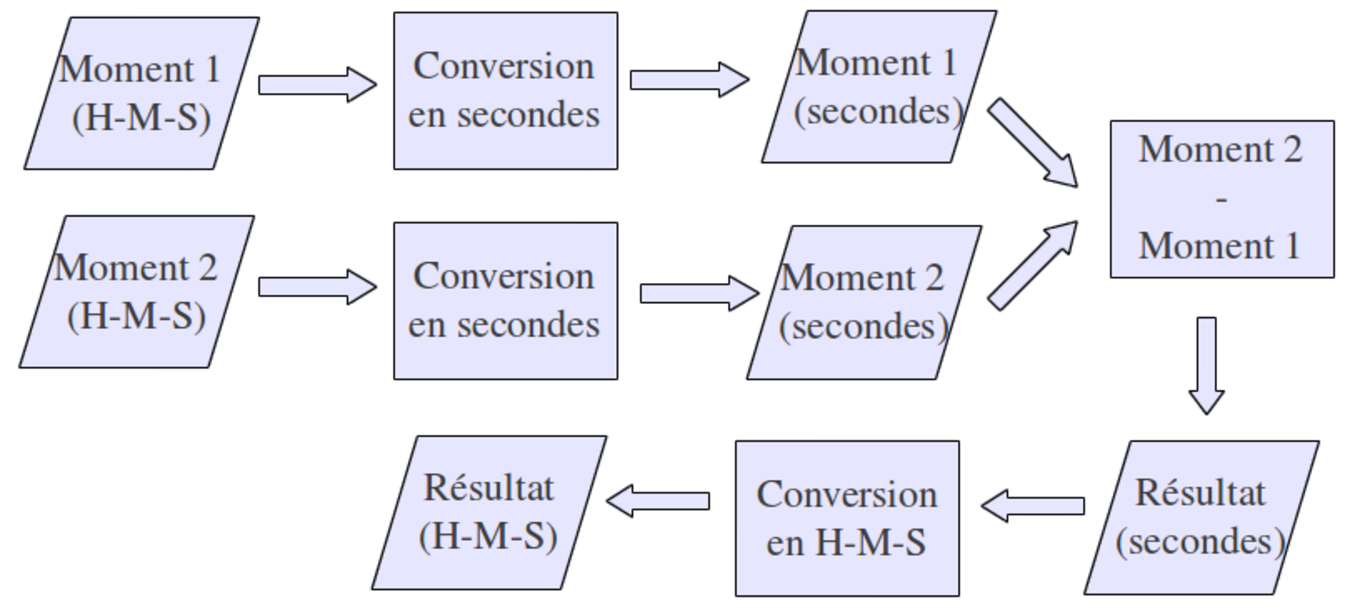
\includegraphics[width=0.8\textwidth]{image/module-conversion}
	\end{center}
\end{frame}

\subsubsection{Conversion en secondes}

\begin{frame}{Écart entre 2 moments}
	Une des sous-tâches est donc la conversion en secondes
	d'un moment exprimé en heures-minutes-secondes
	(h-m-s). 
	
	\bigskip
	
	Il nous faut adapter la solution trouvée pour
	l'exercice du chapitre sur les algorithmes séquentiels
	car il n'est pas question ici que les données soient
	lues ni que le résultat soit écrit~; 
	
	\bigskip
	
	l'interaction ne
	se fait pas avec l'utilisateur mais avec le module
	principal qui va l'utiliser.
\end{frame}

\begin{frame}{Écart entre 2 moments}
	La première question à se poser est donc celle des paramètres~:

	\bigskip
	
	\begin{itemize}
	\item 
		Quelles sont les données dont a besoin l'algorithme
		pour travailler ?
	\item 
		Quels résultats fournit-il ?
	\end{itemize}
\end{frame}

\begin{frame}{Écart entre 2 moments}
	Dans notre cas, la réponse est simple~:

	\bigskip
	
	\begin{itemize}
	\item {
		Les données sont le moment à convertir en secondes. 
		
		Ce moment est
		représenté par trois entiers~: les heures, les minutes et les secondes
		;}
	\item {
		Le résultat est le moment converti en secondes. 
		
		Il est représenté par un entier.}
	\end{itemize}
\end{frame}

\begin{frame}{Écart entre 2 moments}
	Lorsque le résultat est représenté par une seule donnée, on a le choix
	entre un paramètre en sortie~:

	\bigskip
	
	\cadre{
	\begin{pseudo}
		\LComment Affiche trois entiers~: des heures, des minutes et des secondes et sort le nombre de secondes correspondant.
		\ModuleSign{hmsVersSec}{h\In, m\In, s\In, secondes\Out~: entiers}{}
	\end{pseudo}
	}
	
	\bigskip
	
	ou une valeur de retour~:

	\bigskip
	
	\cadre{
	\begin{pseudo}
		\LComment Affiche trois entiers~: des heures, des minutes et des secondes et retourne le nombre de secondes correspondant.
		\ModuleSign{hmsVersSec}{h\In, m\In, s\In~: entiers}{entier}
	\end{pseudo}
	}
\end{frame}

\begin{frame}{Écart entre 2 moments}
		Dans de pareils cas, 
	on privilégie souvent la valeur de retour car cela
	facilite l'écriture lors de l'appel.

	\bigskip
	
	L'algorithme s'écrit alors~:

	\bigskip
	
	\cadre{
	\begin{pseudo}
	\LComment Affiche trois entiers~: des heures, des minutes et des secondes 
	\LComment et retourne le nombre de secondes correspondant.
		\Module{hmsVersSec}{h\In, m\In, s\In~: entiers}{entier}
			\Decl secondes~: entier \RComment {À déclarer puisque ce n'est pas un paramètre}
			\Let secondes \Gets  h * 3600 + m * 60 + s
			\Return secondes
		\EndModule
	\end{pseudo}
	}
\end{frame}

\begin{frame}{Écart entre 2 moments}
	ou de manière équivalente mais plus concise~:

	\bigskip
	
	\cadre{
	\begin{pseudo}
	\LComment Affiche trois entiers~: des heures, des minutes et des secondes 
	\LComment et retourne le nombre de secondes correspondant.
		\Module{hmsVersSec}{h\In, m\In, s\In~: entiers}{entier}
			\Return h * 3600 + m * 60 + s
		\EndModule
	\end{pseudo}
	}
\end{frame}

\subsubsection{Conversion en heures-minutes-secondes}

\begin{frame}{Conversion en heures-minutes-secondes}
	À la fin de notre algorithme, il nous faudra reconvertir un résultat
	exprimé en secondes sous la forme heures-minutes-secondes. 
	
	\bigskip
	
	À nouveau,
	on a déjà résolu ce problème dans le chapitre sur les algorithmes
	séquentiels. 
	
	\bigskip
	
	Mais il faut l'adapter à
	l'usage de paramètres.
\end{frame}

\begin{frame}{Conversion en heures-minutes-secondes}
	\begin{itemize}
	\item {
		Quelles sont les données ? 
		
		Une seule, le moment exprimé en secondes}
		
	\bigskip
	
	\item {
		Quels sont les résultats calculés par le module ? 
		
		Ce même moment exprimé
		en heures-minutes-secondes. 
		
		Trois entiers sont requis ce qui fait que
		le choix entre un paramètre en sortie et une valeur de retour ne se
		pose pas ici~; 
		
		impossible d'utiliser une valeur de
		retour (qui doit être unique)~; 
		
		on doit utiliser des paramètres en
		sortie.}
	\end{itemize}
\end{frame}

\begin{frame}{Conversion en heures-minutes-secondes}
	Ce qui donne~:

	\bigskip
	
	\cadre{
	\begin{pseudo}
		\LComment Affiche un nombre de secondes et sort les heures, les minutes et les secondes correspondant.
		\Module{secVersHMS}{secondes\In, s\Out, m\Out, s\Out~: entiers}{}
			\Let h \Gets secondes DIV 3600
			\Let m \Gets (secondes MOD 3600) DIV 60
			\Let s \Gets secondes MOD 60
		\EndModule
	\end{pseudo}
	}
\end{frame}

\subsubsection{Solution}

\begin{frame}{Solution}
	À présent, on a tout pour écrire la solution à notre problème

	\bigskip
	
	\cadre{
	\begin{pseudo}
		\LComment Lit deux moments (h-m-s) et affiche le moment de la différence entre les deux.
		\Module{différenceEntreHeures}{}{} \RComment Pas de paramètres !
			\Decl h1, m1, s1, h2, m2, s2~: entiers \RComment Les 2 moments à soustraire
			\Decl secondes1, secondes2~: entiers \RComment Ces 2 moments en secondes
			\Decl diffSecondes~: entier \RComment La différence en secondes
			\Decl diffH, diffM, diffS~: entiers \RComment La différence en H-M-S
			\Read h1, m1, s1, h2, m2, s2
			\Let secondes1 \Gets hmsVersSec( h1, m1, s1 )
			\Let secondes2 \Gets hmsVersSec( h2, m2, s2 )
			\Let diffSecondes \Gets secondes2 – secondes1
			\Stmt secVersHMS( diffSecondes, diffH, diffM, diffS )
			\Write diffH, diffM, diffS
		\EndModule
	\end{pseudo}
	}
\end{frame}

\begin{frame}{Solution}
	Dans la solution ci-dessus, 
	quelle est ou quelles sont la/les variable(s) locale(s) 
	dont on pourrait se passer moyennant une réécriture de
	l'algorithme ?
\end{frame}

\subsection{Blocs}

\begin{frame}{Blocs}
	\begin{itemize}
	\item
	Un bloc est l’écriture d’une portion de module
	à l’extérieur de celui-ci. C’est un simple
	{\textit{déplacement}}
	de lignes de codes vers un autre endroit du texte de
	l'algorithme.
	
	\bigskip
	
	\item
	La raison de découper un module en blocs
	peut être le souci de clarifier un algorithme en le découpant en étapes
	bien distinctes.
	
	\bigskip
	
	\item
	Les variables
	d’un bloc ne sont donc pas des variables locales du bloc dans lequel
	elles apparaissent, mais bien des variables locales du module auquel
	appartient ce bloc.
	\end{itemize}
\end{frame}

\begin{frame}{Blocs}
	\begin{itemize}
	\item
	L’appel de l’exécution des instructions se trouvant
	dans un bloc est similaire à celui d’un module avec paramètres, on
	écrit simplement le nom du bloc comme s’il s’agissait d’une
	instruction.
	\end{itemize}
\end{frame}

\begin{frame}{Blocs}
	Pour exemple, le module additionnerFractions (première version dans le
	chapitre 3) pourrait se découper ainsi~:

	\bigskip
	
	\cadre{
	\begin{pseudo}
	\LComment Lit les contenus de 2 fractions et affiche leur somme
		\Module{additionnerFractions}{}{}
			\Stmt déclaration
			\Stmt lectureDonnées
			\Stmt calculs
			\Stmt écritureRésultat
		\EndModule
	\end{pseudo}
	}
\end{frame}

\begin{frame}{Blocs}
	\cadre{
	\begin{pseudo}
	\Block{déclaration}
		\Decl num1, den1, num2, den2, numRes, denRes~: entiers
	\EndBlock
	\end{pseudo}
	}

	\bigskip
	
	\cadre{
	\begin{pseudo}
	\Block{lectureDonnées}
		\Read num1, den1, num2, den2
	\EndBlock
	\end{pseudo}
	}
\end{frame}

\begin{frame}{Blocs}
	\cadre{
	\begin{pseudo}
	\Block{calculs}
		\Let numRes \Gets num1 * den2 + num2 * den1
		\Let denRes \Gets den1 * den2
	\EndBlock
	\end{pseudo}
	}

	\bigskip
	
	\cadre{
	\begin{pseudo}
	\Block{écritureRésultat}
		\Write numRes, "/", denRes \RComment la fraction n'est pas simplifiée
	\EndBlock
	\end{pseudo}
	}
\end{frame}

\subsection{Qu'est-ce qu'un algorithme de qualité ?}

\begin{frame}{Algorithme de qualité}
	\begin{itemize}
	\item
	Nous voulons tous produire du code de qualité mais
	qu'est-ce que cette notion recouvre vraiment ?
	\item
	Qu'est-ce qui permet de juger de la qualité
	d'un code ? 
	\item
	De nombreux critères existent. 
	\end{itemize}
	
	\bigskip
	
	Citons ici,
	parmi les plus pertinents, ceux qui sont le plus liés à ce
	cours.
\end{frame}

\begin{frame}{Algorithme de qualité}
	\begin{itemize}
	\item
		La \textbf{validité}~: le code doit
	réaliser les tâches pour lesquelles 
	il a été écrit, même dans tous les
	cas particuliers imaginés.
	
	\bigskip
	
	\item 
		L'\textbf{extensibilité} (ou évolutivité)~:
	le code doit être écrit de telle sorte qu'un changement
	mineur dans le problème n'implique
	qu'un changement mineur dans le code.
	
	\bigskip
	
	\item
		La \textbf{réutilisabilité}~: c'est
	la capacité de réutiliser 
	un bout de code d’un projet dans un autre projet de 
	façon aisée et sûre.
	\end{itemize}
\end{frame}

\begin{frame}{Algorithme de qualité}
	\begin{itemize}
	\item
		La \textbf{lisibilité}~: 
		
	Au niveau global, on doit facilement comprendre la structure
	générale du code afin de pouvoir aisément comprendre où se trouve 
	la portion de	code qui nous intéresse. 
	
	Au niveau local, on doit pouvoir comprendre
	aisément chaque bout de code.
	
	\bigskip
	
	\item 
		L'\textbf{efficience}~: 
	ce critère s'intéresse à la bonne utilisation des
	ressources informatiques. Est-ce que le programme va tourner
	suffisamment vite, utiliser peu de mémoire ?
	\end{itemize}
\end{frame}

\section{Les tableaux à 2 dimensions}
%\leconwithtoc

\subsection{Définition}

\begin{frame}{Définition}
	\begin{itemize}
		\item
		La \textbf{dimension} d’un tableau est le nombre d’indices qu’on utilise
		pour faire référence à un de ses éléments. 
		\item
		Attention de ne pas confondre avec la	taille !
	\end{itemize}
	
	Dans ce qui précède, nous avons introduit les tableaux à une dimension.
	
	Un seul indice suffisait à localiser un de ses éléments. 
	
	De nombreuses	situations nécessitent cependant 
	l’usage de tableaux à deux dimensions.
	
	Ils vous sont déjà familiers par leur présence dans beaucoup de
	situations courantes : calendrier, grille horaire, grille de mots
	croisés, sudoku, jeux se déroulant sur un quadrillage (damier,
	échiquier, scrabble, \dots).
\end{frame}

\subsection{Déclaration}

\begin{frame}{Déclaration}
	Pour déclarer un tableau statique à 2 dimensions, on écrira :

	\cadre{
	\begin{pseudo}
	\Decl nomTableau : \K{tableau} [ligMin à ligMax, colMin à colMax] de TypeElément
	\end{pseudo}
	}
	
	Pour un tableau dynamique, on procédera en deux étapes comme expliqué
	pour les tableaux à une dimension. 
	
	\cadre{
	\begin{pseudo}
	\Decl nomTableau~: \K{tableau} de TypeElément
	\LComment Le code peut déterminer ici les bornes
	\Let nomTableau \Gets \K{nouveau} \K{tableau} [ligneMin à ligneMax, colMin à colMax] de TypeElément
	\end{pseudo}
	}

	où \code{ligneMin}, \code{ligneMax}, 
	\code{colMin} et \code{colMax}sont des
	expressions entières quelconques.
\end{frame}

\begin{frame}{Déclaration}
	On ne se permettra pas en logique de
	combiner les deux types de tableaux, à savoir utiliser la notation
	«~statique~» pour certaines dimensions et «~dynamique~» pour les
	autres.

	Notez qu'un tableau à deux dimensions peut aussi être
	vu comme un tableau à une dimension dont chacun des éléments est
	lui-même un tableau à une dimension.
\end{frame}

\begin{frame}{Exemple} 
	Soit le tableau déclaré ainsi:

	\cadre{
	\begin{pseudo}
	\Decl ntabLettres : \K{tableau}[1 à 4, 1 à 5] de caractères
	\end{pseudo}
	}

	On peut le visualiser à l’aide d’une grille à 4 lignes et 5 colonnes.
\end{frame}

\begin{frame}{Exemple}
	\begin{center}
	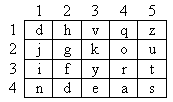
\includegraphics[width=4cm]{image/tab2d-vision-tab2d}
	\end{center}

	Ainsi, la valeur de \code{tabLettres[3,4]} 
	est le caractère ‘r’. 
\end{frame}

\begin{frame}{Exemple}
		La vision «~tableau de tableau~» 
	(ou décomposition en niveaux)
	donnerait :

	\begin{center}
	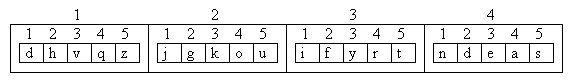
\includegraphics[width=0.9\textwidth]{image/tab2d-vision-tabtab}
	\end{center}

	Dans cette représentation, le tableau \code{tabLettres} est
	d’abord décomposé à un premier niveau en quatre éléments auxquels on
	accède par le premier indice. Ensuite, chaque élément de premier niveau
	est décomposé en cinq éléments de deuxième niveau accessibles par le
	deuxième indice.
\end{frame}

\begin{frame}{Exemple~: Statistiques de vente}
	reprenons l'exemple du stock de 10 produits
	qui a servi d'introduction au chapitre sur les tableaux
	mais, cette fois, pour chaque jour de la semaine.
	
	\begin{small}
	\begin{center}
		\begin{tabular}{*{8}{>{\centering\arraybackslash}m{1.3cm}}}
			~ &
			{article1} &
			{article2} &
			{article3} &
			\dots &
			{article8} &
			{article9} &
			{article10}\\
		\end{tabular}	
		\begin{tabular}{|m{1.3cm}|*{7}{>{\centering\arraybackslash}m{1.3cm}|}}
			\hline
			{lundi} & 
			{cpt[1][1]} &
			{cpt[1][2]} &
			{cpt[1][3]} &
			\dots &
			{cpt[1][8]} &
			{cpt[1][9]} &
			{cpt[1][10]}
			\\\hline
			{mardi} &  
			{cpt[2][1]} &
			{cpt[2][2]} &
			{cpt[2][3]} &
			\dots &
			{cpt[2][8]} &
			{cpt[2][9]} &
			{cpt[2][10]}
			\\\hline
			{mercredi} & 
			{cpt[3][1]} &
			{cpt[3][2]} &
			{cpt[3][3]} &
			\dots &
			{cpt[3][8]} &
			{cpt[3][9]} &
			{cpt[3][10]}
			\\\hline
			{jeudi} & 
			{cpt[4][1]} &
			{cpt[4][2]} &
			{cpt[4][3]} &
			\dots &
			{cpt[4][8]} &
			{cpt[4][9]} &
			{cpt[4][10]}
			\\\hline
			{vendredi} & 
			{cpt[5][1]} &
			{cpt[5][2]} &
			{cpt[5][3]} &
			\dots &
			{cpt[5][8]} &
			{cpt[5][9]} &
			{cpt[5][10]}
			\\\hline
			{samedi} & 
			{cpt[6][1]} &
			{cpt[6][2]} &
			{cpt[6][3]} &
			\dots &
			{cpt[6][8]} &
			{cpt[6][9]} &
			{cpt[6][10]}
			\\\hline
			{dimanche} & 
			{cpt[7][1]} &
			{cpt[7][2]} &
			{cpt[7][3]} &
			\dots &
			{cpt[7][8]} &
			{cpt[7][9]} &
			{cpt[7][10]}
			\\\hline
		\end{tabular}
	\end{center}
	\end{small}
\end{frame}

\begin{frame}{Exemple~: Statistiques de vente}
	\cadre{
	\begin{pseudo}
	\scriptsize{
	\LComment Calcule et affiche la quantité vendue de 10 produits
	\LComment pour chaque jour de la semaine (de 1~: lundi à 7~: dimanche).
	\Module{statistiquesVentesSemaine}{}{}
		\Empty
		\Decl cpt~: \K{tableau} [1 à 7, 1 à 10] d’entiers
		\Decl produit, jour~: entiers
		\Empty
		\Stmt initialiser(cpt)
		\Empty
		\LComment Pour chaque jour de la semaine
		\For{jour \K{de} 1 \K{à} 7}
			\Stmt traiterStock1Jour(cpt, jour)
			\For{produit \K{de} 1 \K{à} 10}
				\Write "quantité vendue de produit ", produit, " ce jour ", jour, "~: ", cpt[jour][i]
			\EndFor
		\EndFor	
	\EndModule
	}
	\end{pseudo}
	}
\end{frame}

\begin{frame}{Exemple~: Statistiques de vente}
	\cadre{
	\begin{pseudo}
	\LComment Ce module initialise le tableau d'entiers à 0
	\Module{initialiser}{entiers\InOut~: \K{tableau} [1 à 7, 1 à 10] d’entiers}{}
		\Decl i, j~: entiers
		\For{i \K{de} 1 \K{à} 7}
			\For{j \K{de} 1 \K{à} 10}
				\Let cpt[i][j] \Gets 0
			\EndFor
		\EndFor
	\EndModule
	\end{pseudo}
	}
\end{frame}

\begin{frame}{Exemple~: Statistiques de vente}
	\cadre{
	\begin{pseudo}
	\scriptsize{
	\LComment Ce module effectue le traitement du stock pour une journée.
	\Module{traiterStock1Jour}{cpt~\InOut: \K{tableau} [1 à 7, 1 à 10] d’entiers, jour~: entier}{}
		\Decl numéroProduit, quantité~: entiers
		\Write "Introduisez le numéro du produit~:"
		\Read numéroProduit
		\Empty
		\While{numéroProduit > 0}
			\Empty
			\Write "Introduisez la quantité vendue~:"
			\Read quantité
			\Empty
			\Let cpt[jour][numéroProduit] \Gets cpt[jour][numéroProduit] + quantité
			\Empty
			\Write "Introduisez le numéro du produit~:"
			\Read numéroProduit
			\Empty
		\EndWhile
	\EndModule
	}
	\end{pseudo}
	}
\end{frame}

\subsection{La troisième dimension (et au-delà)}

\begin{frame}{La troisième dimension (et au-delà)}
	Certaines situations complexes nécessitent l'usage de
	tableaux à 3 voire plus de dimensions.

	Pour déclarer un tableau statique à $k$ dimensions, on écrira :

	\cadre{
	\begin{pseudo}
	\Decl nomTableau : \K{tableau} [ bMin\_1 à bMax\_1, \dots, bMin\_k à bMax\_k] de TypeElément
	\end{pseudo}
	}

	où chaque paire de bornes \code{bMin\_i}~et
	\code{bMax\_i} limite l’indice correspondant 
	à la $i^{ème}$	dimension du tableau.
\end{frame}

\subsection{Parcours d'un tableau à deux dimensions}

\begin{frame}{Parcours d'un tableau à deux dimensions}
	envisageons le parcours des tableaux à deux dimensions 
(n lignes et m colonnes).

Déclaration d'un tableau statique~:

\cadre{
\begin{pseudo}
	\Decl tab~: tableau [1 à n, 1 à m] de T
\end{pseudo}
}

Déclaration d'un tableau dynamique~:

\cadre{
	\begin{pseudo}
	\Decl tab~: \K{tableau} de T
	\Let tab \Gets \K{nouveau} \K{tableau} [1 à n, 1 à m] de T
	\end{pseudo}
}
\end{frame}

\begin{frame}{Parcours d'un tableau à deux dimensions}	
	Commençons par des cas plus simples 
	où on ne parcourt qu'une seule des dimensions 
	puis attaquons le cas général.
\end{frame}

\begin{frame}{Parcours d'un tableau à deux dimensions~: parcours d'une dimension}	
	On peut vouloir ne parcourir qu'une seule ligne du tableau.
	Si on parcourt la ligne $l$, on visite les cases 
	$(l,1)$, $(l,2)$, \dots, $(l,m)$.
	L'indice de ligne est constant et c'est l'indice de colonne qui varie.

	\begin{center}
	$l$
	\begin{tabular}{|*{5}{>{\centering\arraybackslash}m{0.3cm}|}}
	\hline
	\ & \ & \ & \ & \  \\
	\hline
	\cellcolor{gray!25}\ & \cellcolor{gray!25}\ & \cellcolor{gray!25}\ & \cellcolor{gray!25}\ & \cellcolor{gray!25}\  \\
	\hline
	\ & \ & \ & \ & \  \\
	\hline
	\end{tabular}
	\end{center}
\end{frame}

\begin{frame}{Parcours d'un tableau à deux dimensions~: parcours d'une dimension}	
	Ce qui donne l'algorithme :

	\cadre{
	\begin{pseudo}
		\LComment{Parcours de la ligne $l$ d'un tableau à deux dimensions}
		\For{c de 1 à m}
			\Stmt traiter tab[l,c]
		\EndFor
	\end{pseudo}
	}
\end{frame}

\begin{frame}{Parcours d'un tableau à deux dimensions~: parcours d'une dimension}	

	Retenons~: 
	
	\textbf{pour parcourir une ligne, on utilise une boucle sur les colonnes}.

\end{frame}

\begin{frame}{Parcours d'un tableau à deux dimensions~: parcours d'une dimension}	
	Symétriquement, on pourrait considérer le parcours de la colonne $c$
	comme avec l'algorithme suivant.

	\cadre{
	\begin{pseudo}
		\LComment{Parcours de la colonne $c$ d'un tableau à deux dimensions}
		\For{l de 1 à n}
			\Stmt traiter tab[l,c]
		\EndFor
	\end{pseudo}
	}
\end{frame}

\begin{frame}{Parcours d'un tableau à deux dimensions~: parcours d'une dimension}	
	Si le tableau est carré ($n=m$) on peut aussi envisager le parcours
	des deux diagonales.

	Pour la colonne descendante, 
	les éléments à visiter sont $(1,1)$, $(2,2)$, \dots, $(n,n)$.

	\begin{center}
	\begin{tabular}{|*{3}{>{\centering\arraybackslash}m{0.3cm}|}}
	\hline
	\cellcolor{gray!25}\ & \ & \ \\
	\hline
	\ & \cellcolor{gray!25}\ & \ \\
	\hline
	\ & \ & \cellcolor{gray!25}\ \\
	\hline
	\end{tabular}
	\end{center}
\end{frame}

\begin{frame}{Parcours d'un tableau à deux dimensions~: parcours d'une dimension}	
	Une seule boucle suffit comme le montre l'algorithme suivant.

	\cadre{
	\begin{pseudo}
		\LComment{Parcours de la diagonale descendante d'un tableau carré}
		\For{i de 1 à n}
			\Stmt traiter tab[i,i]
		\EndFor
	\end{pseudo}
	}
\end{frame}

\begin{frame}{Parcours d'un tableau à deux dimensions~: parcours d'une dimension}	
	Pour la colonne montante, 
	on peut envisager deux solutions, 
	avec deux indices ou un seul
	en se basant sur le fait que $i+j=n+1 \Rightarrow j=n+1-i$.

	\cadre{
	\begin{pseudo}
		\LComment{Parcours de la diagonale montante d'un tableau carré - 2 indices}
		\Let j \Gets n
		\For{i de 1 à n}
			\Stmt traiter tab[i,j]
			\Let j \Gets j - 1
		\EndFor
	\end{pseudo}
	}
\end{frame}

\begin{frame}{Parcours d'un tableau à deux dimensions~: parcours d'une dimension}	
	\cadre{
	\begin{pseudo}
		\LComment{Parcours de la diagonale montante d'un tableau carré - 1 indice}
		\For{i de 1 à n}
			\Stmt traiter tab[i, n + 1 - i]
		\EndFor
	\end{pseudo}
}
\end{frame}

\begin{frame}{Parcours d'un tableau à deux dimensions~: parcours des deux dimensions}
	Les deux parcours les plus courants sont les parcours ligne par ligne
	et colonne par colonne.
	
	Les tableaux suivants montrent dans quel ordre chaque case est visitée dans ces deux parcours.
\end{frame}

\begin{frame}{Parcours d'un tableau à deux dimensions~: parcours des deux dimensions}
	\begin{center}
	\begin{minipage}{0.4\textwidth}
	\begin{center}
	Parcours ligne par ligne\\
	\begin{tabular}{|*{5}{>{\centering\arraybackslash}m{0.35cm}|}}
	\hline
	1 & 2 & 3 & 4 & 5 \\
	\hline
	6 & 7 & 8 & 9 & 10 \\
	\hline
	11 & 12 & 13 & 14 & 15 \\
	\hline
	\end{tabular}
	\end{center}
	\end{minipage}
	\end{center}
\end{frame}

\begin{frame}{Parcours d'un tableau à deux dimensions~: parcours des deux dimensions}
	\begin{center}
	\begin{minipage}{0.4\textwidth}
	\begin{center}
	Parcours colonne par colonne\\
	\begin{tabular}{|*{5}{>{\centering\arraybackslash}m{0.35cm}|}}
	\hline
	1 & 4 & 7 & 10 & 13 \\
	\hline
	2 & 5 & 8 & 11 & 14 \\
	\hline
	3 & 6 & 9 & 12 & 15 \\
	\hline
	\end{tabular}
	\end{center}
	\end{minipage}
	\end{center}
\end{frame}

\begin{frame}{Parcours d'un tableau à deux dimensions~: parcours des deux dimensions}
	Le plus simple est d'utiliser deux boucles imbriquées 

	\cadre{
	\begin{pseudo}
		\LComment{Parcours d'un tableau à 2 dimensions, ligne par ligne}
		\For{lg de 1 à n}
			\For{col de 1 à m}
				\Stmt traiter tab[lg,col]
			\EndFor
		\EndFor
	\end{pseudo}
	}
\end{frame}

\begin{frame}{Parcours d'un tableau à deux dimensions~: parcours des deux dimensions}
	\cadre{
	\begin{pseudo}
		\LComment{Parcours d'un tableau à 2 dimensions, colonne par colonne}
		\For{col de 1 à m}
			\For{lg de 1 à n}
				\Stmt traiter tab[lg,col]
			\EndFor
		\EndFor
	\end{pseudo}
	}
\end{frame}

\begin{frame}{Parcours d'un tableau à deux dimensions~: parcours des deux dimensions}
	Mais on peut obtenir le même résultat avec une seule boucle
	si l'indice sert juste à compter le nombre de passages
	et que les indices de lignes et de colonnes sont gérés manuellement.

	L'algorithme suivant montre ce que ça donne
	pour un parcours ligne par ligne.
	La solution pour un parcours colonne par colonne est similaire
	et laissée en exercice.
\end{frame}

\begin{frame}{Parcours d'un tableau à deux dimensions~: parcours des deux dimensions}
	\cadre{
	\begin{pseudo}
		\LComment{Parcours d'un tableau à 2 dimensions via une seule boucle}
		\Let lg \Gets 1
		\Let col \Gets 1
		\For{i de 1 à n*m}
			\Stmt traiter tab[lg,col]
			\Let col \Gets col + 1	\RComment Passer à la case suivante
			\If{col > m} \RComment On déborde sur la droite, passer à la ligne suivante
				\Let col \Gets 1
				\Let lg \Gets lg + 1
			\EndIf
		\EndFor
	\end{pseudo}
	}
\end{frame}

\begin{frame}{Parcours d'un tableau à deux dimensions~: interrompre le parcours}
	Comme avec les tableaux à une dimension, 
	envisageons l'arrêt prématuré lors de la rencontre d'une certaine condition.
	
	Et, comme avec les tableaux à une dimension, 
	transformons d'abord nos \K{pour} en \K{tant que}.

	Par exemple, montrons les deux parcours ligne par ligne, avec une et deux boucle(s).

\end{frame}


\begin{frame}{Parcours d'un tableau à deux dimensions~: interrompre le parcours}
	\cadre{
	\begin{pseudo}
		\LComment{Parcours d'un tableau à 2 dimensions, ligne par ligne, via un tant que}
		\Let lg \Gets 1
		\While{lg < n}
			\Let col \Gets 1
			\While{col < m}
				\Stmt traiter tab[lg, col]
				\Let col \Gets col + 1
			\EndWhile
			\Let lg \Gets lg + 1
		\EndWhile
	\end{pseudo}
	}
\end{frame}

\begin{frame}{Parcours d'un tableau à deux dimensions~: interrompre le parcours}
	\cadre{
	\begin{pseudo}
		\LComment{Parcours d'un tableau à 2 dimensions via une seule boucle et un tant que}
		\Let lg \Gets 1
		\Let col \Gets 1
		\Let i \Gets 1
		\While{i $\le$ n*m} \RComment ou "lg $\le$ n" 
			\Stmt traiter tab[lg,col]
			\Let col \Gets col + 1	\RComment Passer à la case suivante
			\If{col > m} \RComment On déborde sur la droite, 
			\RComment passer à la ligne suivante
				\Let col \Gets 1
				\Let lg \Gets lg + 1
			\EndIf
			\Let i \Gets i + 1		
		\EndWhile
	\end{pseudo}
	}
\end{frame}

\begin{frame}{Parcours d'un tableau à deux dimensions~: interrompre le parcours}
	On peut à présent introduire le test comme on l'a fait 
	dans les algorithmes de parcours des tableaux à une dimension.

	\bigskip

	Illustrons-le au travers de deux exemples.
	
	\bigskip
	
	Le premier introduit un test en utilisant un booléen
	alors que le second introduit un test
	sans utiliser de booléen.

\end{frame}

\begin{frame}{Parcours d'un tableau à deux dimensions~: interrompre le parcours}
	\cadre{
	\begin{pseudo}
		\scriptsize{
		\LComment{Parcours avec test d'arrêt - deux boucles et un booléen}
		\Let trouvé \Gets faux
		\Let lg \Gets 1
		\While{lg $<$ n ET NON trouvé}
			\Let col \Gets 1
			\While{col $<$ m ET NON trouvé}
				\If{\textit{tab[lg, col] impose l'arrêt du parcours}}
					\Let trouvé \Gets vrai
				\Else \RComment Ne pas modifier les indices si arrêt demandé
					\Let col \Gets col + 1
				\EndIf
			\EndWhile
			\If{NON trouvé} \RComment Ne pas modifier les indices si arrêt demandé
				\Let lg \Gets lg + 1
			\EndIf
		\EndWhile
	}
	\end{pseudo}
	}
\end{frame}

\begin{frame}{Parcours d'un tableau à deux dimensions~: interrompre le parcours}
	\cadre{
	\begin{pseudo}
		\LComment{Parcours avec test d'arrêt - une boucle et pas de booléen}
		\Let lg \Gets 1
		\Let col \Gets 1
		\Let i \Gets 1
		\While{i $\le$ n*m ET \textit{tab[lg, col] n'impose pas l'arrêt}}  
			\Let col \Gets col + 1	\RComment Passer à la case suivante
			\If{col > m} \RComment On déborde sur la droite, passer à la ligne suivante
				\Let col \Gets 1
				\Let lg \Gets lg + 1
			\EndIf
			\Let i \Gets i + 1		
		\EndWhile
		\LComment Arrêt prématuré si i $\le$ n*m.
	\end{pseudo}
	}
\end{frame}

\begin{frame}{Parcours plus compliqué - le serpent}
	Envisageons un parcours plus difficile illustré par le tableau suivant.

	\begin{center}
	\begin{tabular}{|*{5}{>{\centering\arraybackslash}m{0.35cm}|}}
	\hline
	1 & 2 & 3 & 4 & 5 \\
	\hline
	10 & 9 & 8 & 7 & 6 \\
	\hline
	11 & 12 & 13 & 14 & 15 \\
	\hline
	\end{tabular}
	\end{center}

	Le plus simple est d'adapter l'algorithme de parcours 
	avec une seule boucle
	en introduisant un sens de déplacement, 
	ce qui donne l'algorithme :
\end{frame}

\begin{frame}{Parcours plus compliqué - le serpent}
	\cadre{
	\begin{pseudo}
		\LComment{Parcours du serpent dans un tableau à deux dimensions}
		\Let lg \Gets 1
		\Let col \Gets 1
		\Let depl \Gets 1	\RComment 1 pour avancer, -1 pour reculer
		\For{i de 1 à n*m}
			\Stmt traiter tab[lg, col]
			\If{1 $\le$ col + depl ET col + depl $\le$ m}
				\Let col \Gets col + depl \RComment On se déplace dans la ligne
			\Else
				\Let lg \Gets lg + 1	\RComment On passe à la ligne suivante
				\Let depl \Gets -depl	\RComment et on change de sens
			\EndIf
		\EndFor
	\end{pseudo}
	}
\end{frame}
\section{L'orienté objet}
%\leconwithtoc

\subsection{Objectif}

\begin{frame}{Objectif}
	Dans ce chapitre, nous présentons les bases de la programmation orientée
	objet. 
	
	Nous commençons par expliquer les motivations qui ont amené ce
	type de programmation avant d'entrer dans le vif du
	sujet en explicitant le concept
	d'\textit{encapsulation}. 
	
	Les autres piliers de
	l'orienté objet (\textit{héritage} et
	\textit{polymorphisme}) ne seront pas vus cette année.
\end{frame}

\subsection{Motivation}

\begin{frame}{Motivation}
	Face à la complexité, la démarche est toujours la même~: découper le
	problème en sous-problèmes (qui peuvent à leur tour être découpés) ce
	qui permet

	\begin{itemize}
		\item 
			d'attaquer chaque problème séparément en évitant la
			surcharge cognitive ;
		\item 
			de répartir le travail entre plusieurs personnes ;
		\item 
			de pouvoir réutiliser du travail déjà produit si un sous-problème est
			déjà apparu dans le cadre d'un autre problème ;
		\item 
			de produire un code plus lisible car s'exprimant avec
			des termes de plus haut niveau, 
			plus proches du problème à résoudre.
		\end{itemize}
	\end{frame}

\begin{frame}{Motivation}
			Ainsi, là où un tri devra être fait, 
			on trouvera le mot «~trier~» qui fera référence 
			à la partie de code qui s’occupe du tri. 
			
			Cela va dans le sens d’une plus grande «~abstraction~» du code~: 
			un code qui s’éloigne du langage simpliste 
			compris par le processeur pour s’approcher de la
			pensée humaine et des termes du problème à résoudre.
\end{frame}

\begin{frame}{Motivation}
	Les langages de programmation ont suivi cette approche en permettant
	toujours plus d’abstraction. 
	
	Dans un chapitre précédent, on vous a	présenté 
	\begin{itemize}
		\item
		la notion de module qui permet de découper la tâche à réaliser
		en sous-tâches ainsi que 
		\item
		la notion de structure qui permet de regrouper des données.
	\end{itemize}
	
	Il s'agit là de deux approches	dissociées. 
\end{frame}

\begin{frame}{Motivation}
	C'est cette lacune que se propose de combler
	l'orienté objet~: 
	\begin{itemize}
		\item
		permettre de définir des \textbf{objets} 
		\begin{itemize}
			\item
			(composés de \textbf{données} et
			\item
			\textbf{d'instructions}) 
		\end{itemize}
		\item
		qui sont proches du problème
		à résoudre. 
		\item
		Cela va permettre une meilleure lisibilité et une plus
		grande concision du code. 
	
	\end{itemize}
	
	\bigskip
	
	Ainsi on pourra définir les notions de date,
	d'employé, de fournisseur, de plateau de jeu, de pion,
	de livre, d'emprunteur, de carte à jouer, de chambre,
	de réservation, de vol, de produit, de stock, de ristourne, de facture,
	de panier d'achats, de compte en banque, de banque, de
	client, de portefeuille d'actions, ...
\end{frame}

\subsection{La notion d'objet}

\begin{frame}{Définition}
	Un \textbf{objet} est une entité logicielle qui~:
	
		\begin{itemize}
		\item 
			a une \textbf{identité~}; c'est-à-dire que nous pouvons
			identifier un objet par un nom (tout comme une variable possède un
			nom).
		\item 
			est capable de sauvegarder un \textbf{état}, c'est à
			dire un ensemble d'informations dans des variables
			internes;
		\item 
			répond à des \textbf{messages} précis en déclenchant des activations
			internes appropriées qui peuvent changer l'état de
			l'objet. Ces opérations sont appelées des
			\textbf{méthodes}. Ce sont des fonctions liées à des objets et qui
			précisent le \textbf{comportement} de ces objets.
		\end{itemize}
\end{frame}

\begin{frame}{État}
	Un objet contient de l'information, des données qui
	définissent son état.

	\textbf{Exemples}	
	\begin{itemize}
	\item 
		Pour un produit, l'état peut être~:
		l'intitulé du produit, son code barre, son prix, ... 
	\item 
		Pour un employé, on peut avoir~: son nom, son prénom, son adresse, sa
		date d'embauche, son salaire mensuel, sa fonction, son
		téléphone, ... 
	\item 
		Une carte à jouer a une couleur et une valeur.
	\item 
		L'état d'une date est le jour du
		calendrier qu'elle représente.
	\item 
		L'état d'une heure est le moment de la
		journée qu'elle représente.
	\end{itemize}
\end{frame}
	
\begin{frame}{État}
		L'état d'un objet est mémorisé via des
		variables qu'on appelle des \textbf{attributs}.

\end{frame}
	
\begin{frame}{Attributs~: définition}
	Les \textbf{attributs} d'un objet sont
	l'ensemble des informations se présentant sous forme
	de variables et permettant de représenter l'état
	d'un objet.
	
	\bigskip

	Nous verrons plus loin la syntaxe précise 
	pour définir les attributs d'un objet.

\end{frame}
	
\begin{frame}{Attributs~: exemple}
	\begin{itemize}
		\item 
			L'intitulé d'un produit peut être
			représenté par une chaine. C'est également le cas des
			nom(s) et prénom(s) d'un employé.
		\item 
			La date d'embauche peut être représentée par un «~objet
			date~» (une date est rarement un type primitif du langage utilisé). Un
			attribut d'un objet peut être lui même un objet.
		\item 
			Un moment de la journée peut aussi être un objet représenté par trois
			entiers\footnote{Toutefois, on verra que ce n'est
			peut-être pas la meilleure solution.}~: les heures, les minutes et les
			secondes (en supposant qu'on désire une précision de
			l'ordre de la seconde).
		\item 
			L'adresse d'un employé peut être
			représentée par une seule chaine mais également par un «~objet
			adresse~» (qui contiendrait~: une rue, un numéro, un code postal\dots).
		\end{itemize}
\end{frame}

\begin{frame}{Attention}
	\textbf{Remarque~: }Certaines parties de
		l'état peuvent évoluer au fil du temps.
		D'autres parties sont immuables. 
		Ainsi l'adresse d'une personne peut changer
		mais pas sa date de naissance.
\end{frame}

\begin{frame}{Exercices - attributs}
	\begin{enumerate}
		\item 
			Quel(s) attribut(s) prendriez-vous pour représenter
			(l'état d') une date ?
		\item 
			Et pour un dé à 6 faces ?
		\item 
			Et pour un produit de magasin ?
		\item 
			Et pour une télévision ?
			(on peut en trouver vraiment beaucoup !)
	\end{enumerate}
\end{frame}

\begin{frame}{Comportement}
	Le \textbf{comportement} d'un objet est défini par
	l'ensemble des messages ou requêtes auxquels il peut répondre.

	Pour ce faire, il exécute un module qui pourra
	éventuellement retourner une information à l'émetteur
	du message.
	
	Les messages peuvent interroger l'objet, le modifier,
	lui demander d'agir sur son environnement (afficher du
	texte, modifier un fichier\dots). 
\end{frame}

\begin{frame}{Comportement~: exemples}
	\begin{itemize}
		\item
			Quels «~messages~» peut-on envoyer à une date ? 
			\pause
			On peut lui demander (entre autres) :
			\begin{itemize}
			\item
				des informations sur le jour du mois, le mois, l'année,
				le jour de la semaine ;
			\item
				si elle est antérieure ou non à une autre date ;
			\item
				si elle fait partie d'une année bissextile ;
			\item
				le nombre de jours qui la sépare de la fin de l'année ;
			\item 
				de passer au jour suivant, à la semaine suivante\dots
			\end{itemize}
	\end{itemize}
\end{frame}

\begin{frame}{Comportement~: exemples}
	\begin{itemize}
		\item 
			Et pour un stock de produits ? On peut 
			\pause
			\begin{itemize}
			\item
				lui demander la quantité disponible d'un produit donné ;
			\item
				lui annoncer l'arrivée d'une quantité
				donnée d'un produit donné ;
			\item
				lui indiquer qu'un produit n'existe
				plus (à retirer du stock) ;
			\item 
				lui demander d'enlever une certaine quantité
				d'un produit du stock.
			\end{itemize}
		\end{itemize}
\end{frame}

\begin{frame}{Comportement~: exemples}
	\begin{itemize}
		\item
			Et pour un employé ? On peut
			\pause
			\begin{itemize}
			\item 
				lui demander son adresse, son salaire ou sa fonction\dots
			\item 
				augmenter son salaire ;
			\item 
				le changer de fonction ;
			\item 
				le licencier 
				(penser à prévoir une date de départ dans l'état !).
			\end{itemize}
		\pause
		\item 
			Pour un moment de la journée on peut demander s'il se
			situe le matin ou pas\dots	
		\end{itemize}
\end{frame}

\begin{frame}{Exercices - comportement}
	\begin{enumerate}
		\item
			Quel comportement voyez-vous pour un téléviseur ?
		\item
			Et pour un produit de magasin ?
	\end{enumerate}
\end{frame}

\begin{frame}{Méthode}
	Un message lance l'exécution d'un
	module appelé \textbf{méthode} dans le jargon de
	l'orienté objet.
\end{frame}

\begin{frame}{Méthode~: Exemples}
	\begin{itemize}
		\item
			Pour permettre à une date de passer au jour suivant, nous allons définir
			une méthode qui incrémente le jour du mois en tenant compte
			d'un possible basculement au mois suivant ou à
			l'année suivante.
		\item
			Pour calculer le bénéfice d'un produit, nous allons définir
			une méthode qui, à partir du prix d'achat et du prix de vente,
			calcule le bénéfice.
		\item 
			Pour permettre à un moment d'indiquer
			s'il est le matin ou pas, nous allons définir une
			méthode comme celle-ci (nous verrons plus tard comment
			l'associer aux objets)
	\end{itemize}
\end{frame}

\begin{frame}{Méthode~: Exemples}
	\cadre{
	\begin{pseudo}
		\LComment On suppose que 'heure' est un des attributs utilisés
		\LComment pour représenter l'état (le moment dans la journée)
		\Method{estMatin}{}{booléen}
			\Return heure < 12 
			\LComment on considère que midi est situé l'après-midi
		\EndMethod
	\end{pseudo}
	}
	
	\medskip
	Cet exemple devrait vous sembler familier à deux exceptions près

	\begin{itemize}
		\item
			on utilise le mot «~\textit{méthode}~» en lieu et place de
			«~\textit{module}~» ;
		\item
			les attributs (l'heure ici) ne sont pas passés en
			paramètre. 
			
			Un objet connait déjà son état et donc la valeur de ses
			attributs. 
			
			Nous verrons plus loin la syntaxe précise.
	\end{itemize}
\end{frame}

\begin{frame}{Exercices - méthodes}
	\begin{enumerate}
	\item 
		Dans le comportement d'un téléviseur, on retrouve
		«~éteindre~» et «~allumer~». 
		À quoi ressemblerait le code de ces méthodes ?
	\item 
		Écrivez la méthode qui permet de passer au jour suivant.
	\item 
		Écrivez la méthode qui calcule 
		le bénéfice réalisé lors de la vente d'un produit.
	\end{enumerate}
\end{frame}

\begin{frame}{Activer un comportement}
	Pour activer un comportement d'un objet, 
	il faut lui envoyer un message 
	(ou dit autrement, appeler une de ses méthodes). 
	
	\bigskip
	
	La syntaxe que nous allons utiliser 
	(c'est la plus courante) est la notation pointée.
	
	\bigskip

	\cadre{
	\begin{pseudo}
		\Stmt nomObjet.nomMéthode()
	\end{pseudo}
	}
\end{frame}

\begin{frame}{Activer un comportement~: exemple}
		Supposons que le nom «~maintenant~» 
		désigne un objet contenant un moment de la journée 
		(on verra comment réaliser cela). 
		
		\bigskip
		
		Si on veut savoir si on est le matin, on peut écrire
		
		\bigskip

		\cadre{
		\begin{pseudo}
			\If{maintenant.estMatin()}
				\Stmt ...
			\EndIf
		\end{pseudo}
		}
\end{frame}

\begin{frame}{Exercice – activer un comportement}
	Écrire la portion de code qui allume une télévision 
	(désignée par «~maTélévision~») 
	et puis l'éteint aussitôt après.		
\end{frame}

\begin{frame}{Les paramètres d'un comportement}
		Activer un comportement revient à appeler une méthode de
		l'objet. 
		
		\bigskip
		
		Souvent il est nécessaire
		d'envoyer à l'objet des informations
		complémentaires pour préciser notre demande ce qui se fait via
		l'utilisation des paramètres.
\end{frame}

\begin{frame}{Les paramètres d'un comportement~: Exemple}
		Si on veut modifier le salaire d'un employé, 
		il faut que notre message contienne le nouveau salaire. 
		
		Autrement dit, 
		il faut communiquer ce nouveau salaire à la méthode 
		de changement du salaire.
		
		\bigskip
		
		Ce qui donne la méthode suivante~:

		\cadre{
		\begin{pseudo}
			\Method{modifierSalaire}{nouveauSalaire~: entier}{}
				\Stmt salaire \Gets nouveauSalaire
			\EndMethod
		\end{pseudo}
		}
\end{frame}

\begin{frame}{Exercices – paramètres du comportement}
	\begin{itemize}
	\item 
		Prenons un objet représentant un produit de magasin. 
		Nous supposerons qu'un produit a un \textit{numéro}, 
		un  \textit{libellé}, un \textit{prixAchat}, 
		un \textit{prix de vente} et une \textit{quantitéEnStock}.
		
		\bigskip
		
		Donnez les \textbf{entêtes} des méthodes suivantes 
		qui permettent de~:
		\begin{itemize}
		\item 
			obtenir le prix de vente
		\item 
			calculer le bénéfice
		\item 
			donner la quantité restant en stock
		\item 
			dire si le produit est en rupture de stock.
		\end{itemize}
	\end{itemize}
\end{frame}

\begin{frame}{Exercices – paramètres du comportement}
	\begin{itemize}
	\item 
		Prenons un objet représentant une date du calendrier grégorien. 
		Donnez les entêtes des méthodes suivantes qui permettent de~:
		\begin{itemize}
		\item
			demander le nom du jour correspondant à une date (par exemple lundi, mardi, ...)
		\item 
			savoir si une date est antérieure à une autre
		\item 
			connaitre le nombre de jours (absolu) séparant deux dates.
		\end{itemize}
	\end{itemize}
\end{frame}

\begin{frame}{Exercices – paramètres du comportement}
	\begin{itemize}
	\item 
		Soit deux dates $date1$ et $date2$ ; écrivez la
		portion de code qui utilise les méthodes ci-dessus pour
		\begin{itemize}
			\item 
				vérifier quelle date précède l'autre;
			\item 
				calculer le nombre de jours d'écart entre ces deux
				dates.
		\end{itemize}
		
	\item 
		Précédemment, vous avez défini l'ensemble du
		comportement d'un téléviseur. Écrivez les entêtes des
		méthodes correspondant à ce comportement ainsi qu'une
		portion de code qui les utilise.
	\end{itemize}
\end{frame}

\subsection{L'encapsulation}

\begin{frame}{L'encapsulation}
	Un objet possède un état qui est représenté par des attributs. 
	
	Les bonnes pratiques de la programmation orientée objet préconisent
	fortement que les attributs d'un objet soient
	invisibles en dehors de l'objet. 
	
	Ils ne pourront être accédés qu'au travers 
	du comportement de l'objet, 
	c'est-à-dire via ses méthodes.
\end{frame}

\begin{frame}{L'encapsulation~: définition}
	\textbf{Lorsque les détails de l'implémentation
		d'un objet sont masqués aux autres objets, on dit
		qu'il y a \textbf{encapsulation} des données et du
		comportement des objets.}
\end{frame}

\begin{frame}{L'encapsulation~: Pourquoi une telle recommandation ?}
	Le but est de garantir la cohérence de l'état de l'objet. 
	
	Si on pouvait accéder directement à un attribut 
	(et donc le modifier), 
	on pourrait y mettre une valeur incohérente. 
	
	Par exemple, on pourrait dire que les minutes d'un moment 
	valent -3 ou 75 ou encore que le jour d'une date est 32 !
	
	\bigskip
	
	Dès lors, il nous faudra préciser pour chaque \textbf{membre} 
	(attributs et méthodes) d'un objet s'il est
	\textbf{privé} (inconnu de l'extérieur) ou
	\textbf{public} (connu de l'extérieur). 
\end{frame}

\begin{frame}{L'encapsulation}
	\begin{itemize}
		\item
		Le bon usage impose que tous les attributs soient rendus privés 
		et que les méthodes restent publiques. 
		\item
		Toutefois, on pourra trouver également des méthodes privées. 
		
		Ce sera notamment le cas si plusieurs méthodes d'un objet 
		ont une partie commune ; 
		il sera intéressant de la \textit{factoriser}, 
		c-à-d en faire une méthode privée (ex~: un calcul de maximum).
		\item
		Puisqu'un attribut est privé,
		il est courant pour chacun des attributs de rencontrer 
		une méthode destinée à connaitre la valeur de cet attribut 
		et une autre qui permet de la modifier.
	\end{itemize}
\end{frame}

\begin{frame}{Accesseur et mutateur}
	{definitions~:}
	\begin{itemize}
		\item
		\textbf{Accesseur}~: méthode dont le but est de fournir la valeur d'un attribut.
		\item
		\textbf{Mutateur}~: méthode dont le but est de modifier la valeur d'un attribut.
	\end{itemize}
	
	Par convention, ces méthodes sont nommées \textit{getNom} et 
	\textit{setNom} où «~nom~» est le nom de l'attribut.
	
	Pour un attribut booléen, on pourra préférer \textit{estNom} ou \textit{isNom} 
	au lieu de \textit{getNom}. 
\end{frame}

\begin{frame}{Accesseur et mutateur~: exemple}
	Écrivons l'accesseur et le mutateur pour l'attribut 
	«~heure~» d'un moment de la journée.
	
	\bigskip

	\cadre{
	\begin{pseudo}
		\Method{getHeure}{}{entier}
			\Return heure
		\EndMethod
	\end{pseudo}
	}
	
	\bigskip

	\cadre{
	\begin{pseudo}
		\Method{setHeure}{uneHeure~: entier}{}
			\Stmt heure \Gets uneHeure
		\EndMethod
	\end{pseudo}
	}
\end{frame}

\begin{frame}{Que faire si le paramètre est invalide ?}
	Dans l'exemple précédent, 
	que se passerait-il si le paramètre \textit{uneHeure} vaut 25 ? 
	
	\pause
	
	\bigskip
	
	Une valeur aberrante serait affectée à l'attribut \textit{heure}.

	\pause
	
	Dans le cas de paramètres invalides, 
	la plus mauvaise solution est de ne rien faire. 
	
	Le programme continuerait en croyant que tout s’est bien
	passé et il court à la catastrophe. 
	
	Il est préférable qu’un programme s'interrompe 
	plutôt que de fournir une mauvaise réponse. 
\end{frame}

\begin{frame}{Que faire si le paramètre est invalide ?}
	Cette année, nous nous contenterons d'indiquer
	clairement dans nos codes qu'il s'agit d'une situation anormale 
	via la primitive \textit{erreur} qui arrête le déroulement du
	programme avec une courte explication du problème.
	
	\bigskip

	La syntaxe que nous allons retenir est
	
	\bigskip

	\cadre{
	\begin{pseudo}
		\Stmt \K{erreur} "explication de l'erreur"
	\end{pseudo}
	}
\end{frame}

\begin{frame}{Que faire si le paramètre est invalide ?}
	Ce qui donne~:	
	
	\cadre{
	\begin{pseudo}
		\Method{setHeure}{uneHeure~: entier}{}
			\If{uneHeure < 0 OU uneHeure > 23}
				\Stmt \K{erreur} "heure invalide"
			\EndIf
			\Stmt heure \Gets uneHeure
		\EndMethod
	\end{pseudo}
	}
\end{frame}

\begin{frame}{Exercice - encapsulation}
		Sans le savoir, vous avez déjà défini des accesseurs et des 
		mutateurs pour le téléviseur. 
		
		\begin{itemize}
			\item
			Lesquels ? 
			\item
			En suivant la convention de nom pour les accesseurs et les mutateurs, 
			quels noms auraient-ils dû porter ?
		\end{itemize}
\end{frame}

\subsection{La notion de classe et d'instance}

\begin{frame}{La notion de classe et d'instance}
	Pour pouvoir utiliser des objets nous allons devoir les définir
	(expliciter leur état et leur comportement). 
	
	Cette définition est commune à tous les objets similaires. 
	
	\bigskip
	
	Par exemple tous les moments ont un même comportement 
	et un même type d'état 
	(des heures, des minutes et des secondes).
\end{frame}

\begin{frame}{La notion de classe et d'instance~: définitions}
	\begin{itemize}
	\item
		Une \textbf{classe} est un ensemble d'objets qui ont en
		commun les mêmes méthodes et qui partagent les mêmes types
		d'attributs.
	
	\bigskip
	
	\item
		Une \textbf{instance}
		d'une classe est un objet particulier
		d'une classe qui peut activer les méthodes de la
		classe et qui a des valeurs particulières pour ses attributs.
	\end{itemize}
\end{frame}

\begin{frame}{La notion de classe et d'instance}
	Définir une classe revient à définir un nouveau type de
	données. 
	
	\bigskip
	
	En gros, on peut dire qu'un \textbf{objet
	est à une classe ce qu'une variable est à un type}.
	
	\bigskip
	
	Comprenons bien que les objets d'une même classe ont le
	même «~type~» d'état mais pas le même état proprement
	dit. 
	
	Deux objets «~moment~» représentent tous deux un moment 
	(heures, minutes, secondes) de la journée mais pas (forcement) 
	le même ! 
	
	Ils auront donc les mêmes attributs mais
	avec des valeurs différentes !
\end{frame}

\begin{frame}{Définition d'une classe}
	Nous devons d'abord définir une classe avant de pouvoir
	en instancier les objets que nous voulons utiliser. 
	
	Précisons la syntaxe utilisée pour définir une classe~:

	\cadre{
	\begin{pseudo}
		\Class{NomDeLaClasse}
			\Private
				\LComment liste des attributs (donc privés par convention)
			\Public
				\LComment liste des méthodes publiques
			\Private
				\LComment liste des méthodes privées
		\EndClass
		\LComment Par souci de lisibilité, on pourra indiquer uniquement 
		les signatures des
		\LComment méthodes et donner le code complet des méthodes à 
		la suite de la classe.
	\end{pseudo}
	}
\end{frame}

\begin{frame}{Définition d'une classe~: exemple}
		la classe Moment qui représente un moment de la journée.

		\cadre{
		\begin{pseudo}
			\Class{Moment}
				\Private
					\Decl heure~: entier
					\Decl minute~: entier
					\Decl seconde~: entier
				\Public
					\MethodSign{getHeure}{}{entier}
					\MethodSign{getMinute}{}{entier}
					\MethodSign{getSeconde}{}{entier}
					\MethodSign{setHeure}{uneHeure~: entier}{}
					\MethodSign{setMinute}{uneMinute~: entier}{}
					\MethodSign{setSeconde}{uneSeconde~: entier}{}
					\MethodSign{estMatin}{}{booléen}
			\EndClass
		\end{pseudo}
		}
\end{frame}

\begin{frame}{Définition d'une classe~: exemple}
		la classe Moment qui représente un moment de la journée.

		\cadre{
		\begin{pseudo}
			\Method{estMatin}{}{booléen}
				\Return heure < 12
			\EndMethod
			\Empty
			\LComment + les accesseurs et les mutateurs		
		\end{pseudo}
		}
\end{frame}

\begin{frame}{Instanciation d'une classe}
	«~Instancier~» signifie créer un objet d'une classe.
	
	\bigskip
	
	Cela s'écrit avec l'instruction	\textit{nouveau}. 
	
	\bigskip
	
	Pour lui donner un nom, 
	on l'assigne à une variable déclarée du type de la
	classe.

	\cadre{
	\begin{pseudo}
		\Decl nomObjet~: nomClasse 
		\RComment déclaration de l'objet
		\Let nomObjet \Gets \K{nouveau} nomClasse() 
		\RComment instanciation de l'objet
	\end{pseudo}
	}
\end{frame}

\begin{frame}{Instanciation d'une classe~: Exemple}
	pour créer un moment de la journée~:
		
		\cadre{
		\begin{pseudo}
			\scriptsize{
			\Module{test}{}{}
				\Decl midi~: Moment
				\RComment déclaration
				\Let midi \Gets \K{nouveau} Moment()
				\RComment instanciation
				\Stmt midi.setHeure( 12 )
				\RComment mutateur
				\Stmt midi.setMinute( 0 )
				\RComment " "
				\Stmt midi.setSeconde( 0 )
				\RComment " "
				\If{midi.estMatin()}
					\Write "Midi est considéré comme
					étant encore le matin"
				\Else 
					\Write "Midi est considéré comme
					étant l'après-midi"
				\EndIf
			\EndModule
		}
		\end{pseudo}
		}
\end{frame}

\begin{frame}{Instanciation d'une classe}
	Différence entre les objets et les types de bases~: 
	\begin{itemize}
		\item
		Lorsqu'on déclare une	variable d'un type de base, cela alloue
		automatiquement un espace mémoire pour cette variable.
		\item
		C'est différent avec les objets~: la déclaration
		n'entraine qu'une réservation mémoire
		pour une «~référence~» vers un objet. 
		
		Celui-ci n'existe pas encore. 
		
		Il sera créé (et sa mémoire
		allouée) via une instruction spécifique (\textit{nouveau}). 
		
		On parle de variable «\textit{~dynamique~}». 
		
		Le nom est alors une «~référence~» vers l’objet. 
		\item
		Les avantages de cette dissociation seront
		évidents lorsque nous parlerons de la notion de \textit{constructeur}.
	\end{itemize}
\end{frame}

\begin{frame}{Instanciation d'une classe}
			Après la déclaration, on a~:
		\begin{center}
		\begin{tabular}{m{2.2089999cm}}
		\centering\arraybslash  midi\\\hline
		\multicolumn{1}{|m{2.2089999cm}|}{\centering\arraybslash
		\itshape rien}\\\hline
		\end{tabular}
		\end{center}
\end{frame}

\begin{frame}{Instanciation d'une classe}
		Après l'instanciation (ou création), on a~:
		\begin{center}
		\begin{tabular}{m{2.578cm}m{2.261cm}|m{3.162cm}|}
		\centering  midi &
		\multicolumn{1}{m{2.261cm}}{~
		} &
		\multicolumn{1}{m{3.162cm}}{\centering\arraybslash
		 Moment}\\\hhline{-~-}
		\multicolumn{1}{|m{2.578cm}|}{~
		} &
		\centering \sffamily → &
		\centering\arraybslash  heure = ?\\\hhline{-~~}
		~
		 &
		~
		 &
		\centering\arraybslash  minute = ?\\
		~
		 &
		~
		 &
		\centering\arraybslash  seconde = ?\\\hhline{~~-}
		\end{tabular}
		\end{center}
		
		Remarquez qu'il n'y a pas d'initialisation par défaut, pour le moment.
\end{frame}

\begin{frame}{Instanciation d'une classe}
		Après l'action des mutateurs, on a~:
		\begin{center}
		\begin{tabular}{m{2.578cm}m{2.261cm}|m{3.162cm}|}
		\centering  midi &
		\multicolumn{1}{m{2.261cm}}{~
		} &
		\multicolumn{1}{m{3.162cm}}{\centering\arraybslash
		 Moment}\\\hhline{-~-}
		\multicolumn{1}{|m{2.578cm}|}{~
		} &
		\centering \sffamily → &
		\centering\arraybslash  heure = 12\\\hhline{-~~}
		~
		 &
		~
		 &
		\centering\arraybslash  minute = 0\\
		~
		 &
		~
		 &
		\centering\arraybslash  seconde = 0\\\hhline{~~-}
		\end{tabular}
		\end{center}
\end{frame}

\begin{frame}{Exercices – classe et instance}
	\begin{enumerate}
		\item 
			Pour les produits, vous avez déjà écrit les attributs et les en-têtes des
			méthodes. Regroupez le tout en une classe \textit{Produit}
			\textbf{en respectant les notations que vous venez de voir.}
		\item 
			Écrivez un module qui affiche le prix d'achat d'un produit, son prix 
			de vente hors TVA et son prix de vente TVA comprise.
	\end{enumerate}		
\end{frame}

\subsection{Les constructeurs}

\begin{frame}{Les constructeurs}
	L'encapsulation nous permet de contrôler
	l'état de l'objet et de
	l'empêcher de tomber dans un état invalide. 
	
	\bigskip
	
	Mais qu'en est-il de l'état de départ ?
	
	Est-il valide ?
	
	\bigskip
	
	Il serait bon, lorsqu'on crée un objet (via
	\textit{nouveau}) de pouvoir indiquer l'état
	initial de l'objet et que cet état puisse être validé.
	C'est le rôle précis des constructeurs.
\end{frame}

\begin{frame}{Les constructeurs}
	Un \textbf{constructeur} est une méthode particulière permettant
	d'initialiser les attributs d'un
	objet lors de sa création effective. Elle porte le même nom que sa
	classe et ne retourne pas de valeur.
\end{frame}

\begin{frame}{Les constructeurs}
	Il peut y avoir plusieurs constructeurs ce qui permet
	d'offrir plusieurs possibilités d'indiquer l'état initial de
	l'objet. Toutefois, nous limiterons au maximum le nombre 
	de constructeurs dans une classe.
	
	\bigskip
	
	Remarquez que cela demande de définir plusieurs méthodes 
	qui portent le même nom. 
	
	C'est ce qu'on appelle la	\textbf{surcharge}. 
	
	Des méthodes homonymes (c-à-d de même nom) doivent
	pouvoir être différenciées via leur signature (la liste de leurs
	paramètres).
\end{frame}

\begin{frame}{Les constructeurs~: Exemple}
	Écrivons des constructeurs pour un moment de la journée~:

	\cadre{
	\begin{pseudo}
		\scriptsize{
		\Class{Moment}
			\Private
				\LComment pas de changement
				\Decl heure~: entier
				\Decl minute~: entier
				\Decl seconde~: entier
			\Public
				\ConstrSign{Moment}{uneHeure, uneMinute, uneSeconde~: entiers}
				\ConstrSign{Moment}{uneHeure, uneMinute~: entiers}
				\RComment 0 seconde par défaut
				\ConstrSign{Moment}{uneHeure~: entier}
				\RComment initialiser à une heure pile
				\Empty
				\LComment pas de changement au niveau des méthodes~:
				\MethodSign{getHeure}{}{entier}
				\MethodSign{getMinute}{}{entier}
				\MethodSign{getSeconde}{}{entier}
				\MethodSign{setHeure}{uneHeure~: entier}{}
				\MethodSign{setMinute}{uneMinute~: entier}{}
				\MethodSign{setSeconde}{uneSeconde~: entier}{}
				\MethodSign{estMatin}{}{booléen}
		\EndClass
		}
		\end{pseudo}
	}
\end{frame}

\begin{frame}{Les constructeurs~: Exemple}
	\cadre{
	\begin{pseudo}
		\scriptsize{
		\Constr{Moment}{uneHeure, uneMinute, uneSeconde~: entiers}
			\Stmt setHeure(uneHeure)
			\Stmt setMinute(uneMinute)
			\Stmt setSeconde(uneSeconde)
		\EndConstr
		
		\Empty
		\Constr{Moment}{uneHeure, uneMinute~: entiers}
			\Stmt setHeure(uneHeure)
			\Stmt setMinute(uneMinute)
			\Stmt setSeconde(0)
		\EndConstr
		
		\Empty
		\Constr{Moment}{uneHeure~: entier}
			\Stmt setHeure(uneHeure)
			\Stmt setMinute(0)
			\Stmt setSeconde(0)
		\EndConstr
		}
					
		\Empty
		\LComment + les accesseurs, les mutateurs et les autres méthodes
	
	\end{pseudo}
	}
\end{frame}

\begin{frame}{Les constructeurs~: Logique vs Java}
	Contrairement à ce qu'on peut trouver dans certains langages, 
	comme Java par exemple, nous n'autorisons pas ici d'appel 
	d'un constructeur d'une classe \textit{A} dans un autre constructeur 
	de cette même classe \textit{A}.
	
	\bigskip
	
	Par contre, il est courant en logique qu'un constructeur 
	appelle les mutateurs afin d'effectuer les tests sans 
	avoir à les dupliquer.
	Mais c'est une démarche que vous éviterez de faire dans
	des langages comme Java par exemple 
	(cela vous sera expliqué plus tard).
	
\end{frame}

\begin{frame}{Les constructeurs~: appels}
	Lorsqu'on instancie un objet, les paramètres
	qu'on donne déterminent le constructeur qui est
	effectivement utilisé pour initialiser l'état de
	l'objet.

	\textbf{Exemple}~: Instancions quelques moments de la journée.
	
	\cadre{
	\begin{pseudo}
		\Let heureDépart \Gets \K{nouveau} Moment(14, 23, 56)
		\Let heureLever \Gets \K{nouveau} Moment(9, 30)
		\Let heureGouter \Gets \K{nouveau} Moment(17)
	\end{pseudo}
	}
\end{frame}


\begin{frame}{Les constructeurs}
	Le fait qu'un objet est instancié via la primitive
	\textit{nouveau} et pas implicitement à la déclaration permet de
	postposer sa construction effective au moment où
	l'état initial qu'on veut lui donner
	sera connu (ce qui peut résulter d'un calcul). On est
	ainsi assuré que tous les objets manipulés sont valides ce qui permet
	d’éviter les situations où une méthode fait des dégâts suite à la
	manipulation d’un objet invalide.
\end{frame}

\begin{frame}{Exercices - constructeur}
		\begin{enumerate}
			\item {
				Écrivez un ou des constructeur(s) pour un \textit{Produit}}
			\item {
				Adaptez le module écrit plus haut pour qu'il affiche le prix hors TVA
				puis le prix TVA comprise du produit n°105176 (Lego réveil figurine policier)
				au prix d'achat de 25\texteuro, au prix de vente de 30\texteuro et 
				dont il y a 10 exemplaires en stock.}
		\end{enumerate}
\end{frame}

\subsection{Du choix de la représentation de l'état}

\begin{frame}{Du choix de la représentation de l'état}
	Lorsqu'on définit une classe, il faut choisir les
	attributs qui vont permettre de représenter l'état des
	objets. Cela peut paraitre immédiat mais il n'en est
	rien.
\end{frame}

\begin{frame}{Du choix de la représentation de l'état~: exemple}
	Pour un moment de la journée, nous avons choisi
	d'utiliser trois attributs entiers (les heures, les
	minutes et les secondes). Nous aurions tout aussi bien pu choisir
	d'utiliser un seul entier représentant le nombre de
	secondes écoulées depuis minuit.
	
	\bigskip
	
	Ces deux représentations sont tout-à-fait équivalentes en terme de
	potentiel mais la grande différence est l'efficacité
	du code des méthodes. 
\end{frame}

\begin{frame}{Du choix de la représentation de l'état}
	Prenons deux méthodes symptomatiques~: celle qui donne
	l'heure et celle qui compare deux moments de la
	journée. La première est beaucoup plus simple à écrire et plus rapide
	avec la première représentation alors que la seconde méthode est plus
	simple à écrire et plus rapide avec la seconde représentation.
	
	\bigskip
	
	Dès lors, quelle représentation choisir ? Il faut examiner, pour chaque
	représentation possible, le nombre de méthodes qui sont efficaces mais
	aussi imaginer la fréquence de leur utilisation (ce qui est difficile
	et changeant). Heureusement, ce choix n'est pas
	définitif. Si on change d'avis, on peut changer la
	représentation. Il faudra bien sûr réécrire les méthodes de la classe
	mais il ne faudra rien changer au reste du code, c-à-d les lignes du
	code utilisant la classe. C’est d’ailleurs là une des grandes forces de
	la programmation orientée objet.
\end{frame}

\begin{frame}{Exercices – représentation de l'état}
		\begin{enumerate}
			\item 
				Compléter la classe Moment en écrivant la méthode «~getHeure~» et celle
				qui compare deux moments pour les deux représentations imaginées
				ci-dessus.
			\item 
				Écrire le module qui crée deux moments de la journée et vérifie si le
				premier est avant le second. Ce code dépend-il des attributs choisis
				pour définir la classe Moment ?
		\end{enumerate}
\end{frame}

\begin{frame}{Remarque}
	Précédemment, nous avons défini un \textbf{accesseur} comme une méthode
	permettant d’accéder à la valeur d’un attribut. 
	
	Mais c’est au	développeur de définir quels sont les attributs ; 
	c’est totalement caché à l’utilisateur de la classe. 
	
	On voit donc bien que cette notion
	d’accesseur n’a pleinement de sens qu’en interne, pour le développeur
	de la classe. 
	
	Pour l’utilisateur il s’agit d’une méthode comme les autres.
\end{frame}

\subsection{La mort d'un objet}

\begin{frame}{La mort d'un objet}
	On sait que déclarer une variable ou créer un objet réserve de l’espace
	en mémoire. On ne s’est jamais demandé quand cet espace mémoire est
	libéré.
	
	\bigskip
	
	Pour les variables locales d’un module ou d'une
	méthode, la réponse est simple~: l’espace mémoire est récupéré
	lorsqu’on arrive à la fin du module ou de la méthode.
	
	\bigskip
	
	Pour les objets, c’est un peu plus compliqué. L’espace réservé pour
	contenir la référence (voir paragraphe suivant) est bien libéré à la
	fin du module puisque la variable cesse d’exister. Par contre l’espace
	réservé dynamiquement pour contenir l’objet lui-même (par la primitive
	\textit{nouveau}) est toujours là et bien là !
	
\end{frame}

\begin{frame}{La mort d'un objet}
	Mais alors, il n’est plus référencé et donc plus utilisable ? Pas
	forcément. En effet, il est possible qu’il soit référencé par plusieurs
	références. Si certaines sont détruites, il se peut que d’autres
	continuent à exister. Ce sera le cas, par exemple, si l’objet constitue
	la valeur de retour de la méthode ; sa référence à l’intérieur du
	module est détruite mais il sera toujours accessible par une référence
	du module appelant.
	
	\bigskip
	
	Mais que faire quand on n’a plus besoin d’un objet ? On trouve
	typiquement deux approches dans les langages OO.
\end{frame}

\begin{frame}{La mort d'un objet~: destruction explicite de l’objet}
	C’est auprogrammeur lui-même de détruire explicitement un objet
	et ainsi de permettre au système de récupérer l’espace mémoire. 
	
	\bigskip
	
	Cette technique offre au programmeur un grand contrôle sur l’utilisation
	de la mémoire mais offre malheureusement quelques inconvénients.
	
	\bigskip

	\begin{itemize}
		\item 
			Cela demande une grande attention lors de la programmation afin de
			récupérer tout l’espace qui peut l’être. Dans le cas contraire, on
			gaspille de la mémoire.
		\item 
			Dans l’autre sens, il ne faut pas trop détruire. Si, par mégarde, on
			détruit un objet qui est encore référencé et qu'on
			utilise cette référence, le comportement du programme est imprévisible
			(la mémoire peut avoir été utilisée pour autre chose).
		\item 
			Un objet peut contenir des références à d’autres objets. La destruction
			est alors un processus non trivial qui peut sensiblement alourdir et
			obscurcir le code.
	\end{itemize}
\end{frame}

\begin{frame}{La mort d'un objet~: utilisation d’un garbage collector (ramasse-miettes)}
	Cette autre approche (choisie notamment par Java) enlève au programmeur
	toute (ou presque) responsabilité quant à la gestion de la mémoire. De
	temps en temps, ou lorsque le besoin s’en fait sentir, un composant du
	système appelé \textit{garbage collector} se met au travail. Son rôle
	est justement de récupérer l’espace qui n’est plus utilisé. Pour cela,
	il considère que tout objet qui n'est plus accessible
	(parce que plus aucune référence ne permet d’y accéder) peut être
	détruit.
	
	\bigskip
	
	Par facilité et parce que cela correspond au cours de Java que vous
	suivez cette année, nous adopterons dans ce cours cette seconde
	approche, c'est à dire qu'il ne faut
	pas se préoccuper de ce problème ;-)

\end{frame}

\subsection{Quelques éléments de syntaxe}

\begin{frame}{Quelques éléments de syntaxe}
	Clarifions certaines notations liées aux objets.

	\begin{itemize}	
		\item {
			On peut directement afficher un objet. Cela affiche son état,
			c'est-à-dire les valeurs de ses attributs dans
			l'ordre où ils apparaissent dans la définition de la
			classe.
			\\
			\bigskip
			\cadre{
			\begin{pseudo}
				\Decl rendezVous~: Moment
				\Let rendezVous \Gets \K{nouveau} Moment(14, 23, 56)
				\Write rendezVous 
				\RComment affichera 14, 23 et 56 dans un format lisible quelconque
			\end{pseudo}
			}
		}
	\end{itemize}
\end{frame}

\begin{frame}{Quelques éléments de syntaxe}
	\begin{itemize}	
		\item {
			Un nom d'objet est en fait une \textbf{référence} à
			l'objet. Ainsi l'affectation ne copie
			pas l'objet mais sa référence. Au final, nous avons
			deux noms identifiant le même objet}
			\\
			\bigskip
			\cadre{
			\begin{pseudo}
				\Decl moment1, moment2~: Moment
				\Let moment1 \Gets \K{nouveau} Moment(14, 23, 56)
				\Let moment2 \Gets moment1
				\RComment moment1 et moment2 désignent le même objet
				\Stmt moment2.setHeure( 12 )
				\Write moment1.getHeure() 
				\RComment affiche 12 !!!
			\end{pseudo}
			}
	\end{itemize}
\end{frame}

\begin{frame}{Quelques éléments de syntaxe}
			\begin{center}
			\tablehead{}
			\begin{supertabular}{m{2cm}m{2cm}|m{2.5cm}|m{2cm}m{2cm}}
			\hhline{-~-~-}
			\multicolumn{1}{|m{2cm}|}{\centering  moment1}
			&
			\centering \sffamily → &
			\centering  Heure = \sout{14} 12 &
			\multicolumn{1}{m{2cm}|}{\centering \sffamily
			←} &
			\multicolumn{1}{m{2.5cm}|}{\centering\arraybslash
			 moment2}\\\hhline{-~~~-}
			~
			 &
			~
			 &
			\centering  minute = 23 &
			~
			 &
			~
			\\
			~
			 &
			~
			 &
			\centering  seconde = 56 &
			~
			 &
			~
			\\\hhline{~~-~~}
			\end{supertabular}
			\end{center}
\end{frame}

\begin{frame}{Quelques éléments de syntaxe}
	\begin{itemize}	
		\item 
			Le signe «~=~» permet de tester que deux noms référencent le même objet.
			Pour tester que deux objets différents sont dans le même état, on
			utilise la méthode «~égal~».
	\end{itemize}
\end{frame}

\begin{frame}{Quelques éléments de syntaxe}
			\cadre{
			\begin{pseudo}
				\Decl moment1, moment2, moment3~: Moment
				\Empty
				\Let moment1 \Gets {nouveau} Moment( 14, 23, 56 )
				\Let moment2 \Gets moment1 
				\LComment moment1 et moment2 désignent le même objet
				\Empty
				\Let moment3 \Gets {nouveau} Moment( 14, 23, 56 )
				\Write moment1 = moment2
				\RComment vrai
				\Write moment1 = moment3 
				\RComment faux
				\Write moment1.égal(moment2) 
				\RComment vrai
				\Write moment1.égal(moment3) 
				\RComment vrai
				\Empty 
				\Stmt moment2.setHeure( 12 )
				\Write moment1.égal(moment2) 
				\RComment vrai
				\Write moment1.égal(moment3) 
				\RComment faux
			\end{pseudo}
			}
\end{frame}

\begin{frame}{Quelques éléments de syntaxe}
	\begin{itemize}
		\item 
			\textbf{Un attribut privé n'est pas connu en dehors de la
			classe.}
			
			Précisons~: un attribut privé n'est connu que
			des instances de cette classe, ce qui signifie qu'il
			est également connu par tous les autres objets de la même
			classe.
			
			\smallskip
			\textbf{Exemple}~: 	
			écrivons la méthode qui teste si un moment précède un
			autre (en supposant que l'état est représenté par un
			seul entier, totalSecondes, le nombre de secondes depuis minuit)
	\end{itemize}
\end{frame}

\begin{frame}{Quelques éléments de syntaxe}
			\cadre{
			\begin{pseudo}
				\Method{estAntérieur}{autre~: Moment}{booléen}
					\Return totalSecondes < autre.totalSecondes
					\LComment c'est équivalent à \textit{retourner} 
					\LComment totalSecondes < autre.getTotalSecondes()
				\EndMethod
			\end{pseudo}
			}
\end{frame}

\begin{frame}{Quelques éléments de syntaxe}
	\begin{itemize}
		\item 
			Lorsqu'il est déclaré, un nom d'objet
			ne référence encore aucun objet. Cela s'indique par la
			valeur «~rien~». On peut aussi utiliser cette valeur pour enlever toute
			référence vers un objet.
	\end{itemize}
\end{frame}

\begin{frame}{Quelques éléments de syntaxe}
			\cadre{
			\begin{pseudo}
				\Decl moment~: Moment
				\RComment moment = rien
				\Let moment \Gets \K{nouveau} Moment( 14, 23, 56 )
				\RComment moment ${\neq}$ rien
				\Let moment \Gets rien
				\RComment moment = rien
			\end{pseudo}
			}
\end{frame}

\begin{frame}{Exercice~: méthode égal}
		Écrire la méthode \textit{égal()} pour la classe \textit{Moment}.
		
		N.B.~: On supposera par la suite qu'une telle méthode
		existe par défaut pour toutes les nouvelles classes.
\end{frame}

\subsection{Représentation modélisée d'une classe}

\begin{frame}{Représentation modélisée d'une classe}
	Un dessin étant souvent plus lisible qu'un texte, on
	peut représenter graphiquement une classe. Une notation courante est
	celle utilisée en UML(Unified
	Modeling Langage). On vous en parlera plus en détail au cours
	d'Analyse. 
	
	\bigskip
	
	Pour faire simple, une classe est
	représentée par un rectangle composé de 3 zones~: la première pour le
	nom de la classe, la deuxième pour les attributs et la troisième pour
	les méthodes. On indique par un signe «~+~» (resp. «~-~») que le membre
	est public (resp. privé)
\end{frame}

\begin{frame}{Représentation modélisée d'une classe}
		\textbf{Exemple}
	
	\begin{center}
	\begin{tabular}{|m{7cm}|}
	\hline
	\centering\arraybslash \bfseries Moment\\\hline
	{ {}- heure~: entier}
	
	{ {}- minute~: entier}
	
	 {}- seconde~: entier\\\hline
	{ + getHeure() \textsf{→} entier}
	
	{ + setHeure( uneHeure~: entier )}
	
	{ + avancer1Heure()}
	
	 ...\\\hline
	\end{tabular}
	\end{center}

	\bigskip

	Remarquons qu'on indique la signature des méthodes mais
	pas le code associé. En fonction du niveau de détail désiré, on
	pourrait aussi omettre les paramètres et types de retour.
\end{frame}

\subsection{Un exemple complet~: une durée}

\begin{frame}{Un exemple complet~: une durée}
	Examinons un exemple complet. 
	
	Vous avez écrit quelques modules manipulant des heures (conversion du format
	HMS en nombre de secondes depuis minuit, conversion inverse, différence
	entre 2 heures, …). 
	
	Il est souvent utile, lorsqu’on développe un
	algorithme, d’avoir à sa disposition un tel type de données au même
	titre que les types prédéfinis. 
	
	Faisons-le !
\end{frame}

\begin{frame}{Un exemple complet~: une durée}
	Avant tout, il faut bien préciser ce que l’on veut décrire. L’«~heure~»
	est un concept multifacettes. Parle-t-on de l’heure comme moment dans
	la journée ou de l’heure comme représentant une durée ? Dans le premier
	cas, elle ne peut dépasser 24h et la différence entre 2 heures n’a pas
	de sens (ou plus précisément n’est pas une heure, mais une durée !).
	Dans le deuxième cas, on n’a pas ces contraintes. Nous allons ici
	adopter la deuxième approche et pour bien la distinguer, nous allons
	plutôt appeler cela une \textbf{durée}.
\end{frame}

\begin{frame}{Un exemple complet~: une durée~: les méthodes}
	La première question à se poser est celle des services qu’on veut
	fournir, c’est-à-dire des méthodes publiques de la classe. On doit
	pouvoir \textit{construire} une durée. On doit pouvoir connaitre le
	nombre de jours, d’heures, minutes ou secondes correspondant à une durée. On doit
	pouvoir effectuer des calculs avec des durées (addition, soustraction).
	Enfin, on doit pouvoir comparer des durées. Arrêtons-nous là, mais en
	pratique, on pourrait trouver encore bon nombre d’autres méthodes qu’il
	serait intéressant de fournir. Ce qui nous donne jusqu’à présent~:
\end{frame}

\begin{frame}{Un exemple complet~: une durée~: les méthodes}
		\cadre{
		\begin{pseudo}
		\scriptsize{
			\Class{Durée}
				\Private
					\LComment rien encore
				\Public
					\ConstrSign{Durée}{secondes~: entier}
					\ConstrSign{Durée}{heure, minute, seconde~: entiers}
					\MethodSign{getJour}{}{entier}
					\RComment nb de jours dans une durée
					\MethodSign{getHeure}{}{entier}
					\RComment entier entre 0 et 23 inclus
					\MethodSign{getMinute}{}{entier}
					\RComment entier entre 0 et 59 inclus
					\MethodSign{getSeconde}{}{entier}
					\RComment entier entre 0 et 59 inclus
					\MethodSign{getTotalHeures}{}{entier}
					\RComment Le nombre total d’heures
					\MethodSign{getTotalMinutes}{}{entier}
					\RComment Le nombre total de minutes
					\MethodSign{getTotalSecondes}{}{entier}
					\RComment Le nombre total de secondes
					\MethodSign{ajouter}{autreDurée~: Durée}{}
					\MethodSign{différence}{autreDurée~: Durée}{Durée}
					\MethodSign{égale}{autreDurée~: Durée}{booléen}
					\MethodSign{plusPetit}{autreDurée~: Durée}{booléen}
			\EndClass
		}
		\end{pseudo}
		}
\end{frame}

\begin{frame}{Un exemple complet~: une durée}
	\textbf{Quelques remarques}
		\begin{itemize}
			\item {
				On a deux constructeurs, ce qui offre plus de souplesse pour initialiser
				un objet. Ceci est un exemple supplémentaire du concept de
				«\textbf{~surcharge~}».}
			\item {
				Faisons bien la distinction entre les méthodes
				\textit{getXXX()} et \textit{getTotalXXX()}. Par
				exemple, la méthode \textit{getMinute()} retourne la valeur
				de la composante «~minutes~» dans une représentation HMS tandis que la
				méthode \textit{getTotalMinutes()} retourne le nombre total
				de minutes entières pour cette durée. Ex~: pour 1h23’12’’,
				\textit{getMinute()} retourne 23 et
				\textit{getTotalMinutes()} retourne 83. Idem avec 
				les jours, les heures	et les secondes.}
		\end{itemize}
\end{frame}

\begin{frame}{Un exemple complet~: une durée}
	\begin{itemize}
			\item {
				Les méthodes \textit{getTotalXXX()} retournent le nombre
				(toujours entier) de XXX contenus dans la durée. 
				
				Exemple, avec la durée
				0h23’52'’, \textit{getTotalMinutes()}
				retourne 23 et pas 24 (autrement dit, il n’y a pas d’arrondi vers le
				haut).}
			\item {
				Il n’y a pas de \textit{mutateur }(\textit{setXXX()}). Ce qui
				signifie qu’on ne peut pas changer directement la valeur de l’objet
				après son initialisation. On aurait pu en définir mais nous
				n'avons pas jugé utile de le faire dans ce cas
				précis.}
	\end{itemize}
\end{frame}

\begin{frame}{Un exemple complet~: une durée}
	\begin{itemize}
			\item {
				La méthode \textit{ajouter()} ne retourne rien. En effet,
				elle ajoute la durée à l’objet sur lequel est appelée la méthode. C’est
				un choix ; on aurait aussi pu dire que la méthode ne modifie pas
				l’objet mais en retourne un autre qui représente la somme. Dans ce cas,
				on l’aurait plutôt appelée «\textit{~plus( )}~».}
			\item {
				La méthode \textit{différence()}, elle, renvoie toujours une
				durée (positive).}
		\end{itemize}
\end{frame}

\begin{frame}{Un exemple complet~: une durée~: les attributs}
	La question suivante est~: «~Comment représenter une durée en interne~?~». 
	Plusieurs possibilités existent. 
	
	Par exemple~:	
		\begin{itemize}
			\item 
				via le nombre d’heures, de minutes et de secondes
			\item 
				via le nombre total de secondes
			\item 
				via une chaine, par exemple au format «~HH~:MM~:SS~» où HH pourrait
				éventuellement excéder 23.
		\end{itemize}
\end{frame}

\begin{frame}{Un exemple complet~: une durée}
	Le premier choix semble le plus évident mais réfléchissons-y de plus
	près. D’une part, pourquoi se limiter aux heures. 
	
	On pourrait
	introduire un champ ‘\textit{jour}’ (après tout on a bien
	une méthode \textit{getJour()}). 
	
	\bigskip
	
	Quel critère doit vraiment nous permettre de décider ? 
	
	Il faut une
	représentation qui soit suffisante (tout est représenté) et qui
	permette d’écrire des méthodes lisibles et si possible efficaces
	(c'est-à-dire où le calcul est rapide). 
	
	Selon ces
	critères, la deuxième représentation est de loin la meilleure. Ce qui
	nous donne~:
\end{frame}

\begin{frame}{Un exemple complet~: une durée}
		\cadre{
		\begin{pseudo}
			\Class{Durée}
				\Private
					\Decl totalSecondes~: entier
				\Public
					\LComment idem
			\EndClass
		\end{pseudo}
		}		
\end{frame}

\begin{frame}{Un exemple complet~: une durée~: l'implémentation}
	On est à présent prêt pour écrire le code des méthodes. Ce qui nous
	donne pour la classe dans son entièreté~:
\end{frame}

\begin{frame}{Un exemple complet~: une durée~: l'implémentation}
	\cadre{
		\begin{pseudo}
			\scriptsize{
			\Class{Durée}
				\Private
					\Decl totalSecondes~: entier
				\Public
					\ConstrSign{Durée}{secondes~: entier}
					\ConstrSign{Durée}{heure, minute, seconde~: entiers}
					\Empty
					\MethodSign{getJour}{}{entier}
					\RComment nb de jours dans une durée
					\MethodSign{getHeure}{}{entier}
					\RComment entier entre 0 et 23 inclus
					\MethodSign{getMinute}{}{entier}
					\RComment entier entre 0 et 59 inclus
					\MethodSign{getSeconde}{}{entier}
					\RComment entier entre 0 et 59 inclus
					\Empty
					\MethodSign{getTotalHeures}{}{entier}
					\RComment Le nombre total d’heures
					\MethodSign{getTotalMinutes}{}{entier}
					\RComment Le nombre total de minutes
					\MethodSign{getTotalSecondes}{}{entier}
					\RComment Le nombre total de secondes
					\Empty
					\MethodSign{ajouter}{autreDurée~: Durée}{}
					\MethodSign{différence}{autreDurée~: Durée}{Durée}
					\MethodSign{égale}{autreDurée~: Durée}{booléen}
					\MethodSign{plusPetit}{autreDurée~: Durée}{booléen}
			\EndClass
			}
		\end{pseudo}
		}
\end{frame}

\begin{frame}{Un exemple complet~: une durée~: l'implémentation}
		\cadre{
		\begin{pseudo}
			\Constr{Durée}{secondes~: entier}
				\If{secondes < 0}
					\Stmt \K{erreur} "paramètre négatif"
				\EndIf
				\Let totalSecondes \Gets secondes
			\EndConstr
			\Empty
			\Constr{Durée}{heure, minute, seconde~: entiers}
				\If{heure < 0 OU minute < 0 OU seconde < 0}
					\Stmt \K{erreur} "un des paramètres est négatif"
				\EndIf
				\Let totalSecondes \Gets 3600*heure + 60*minute + seconde
			\EndConstr
		\end{pseudo}
		}
\end{frame}

\begin{frame}{Un exemple complet~: une durée~: l'implémentation}
		\cadre{
		\begin{pseudo}
			\LComment Retourne le nombre de jours dans une 
			représentation JJ/HH:MM:SS
			\Method{getJour}{}{entier}
				\Return totalSecondes DIV (3600*24)
			\EndMethod
			\Empty
			\LComment Retourne le nombre d'heures dans une 
			représentation JJ/HH:MM:SS
			\Method{getHeure}{}{entier}
				\LComment On doit enlever les jours éventuels
				\Return (totalSecondes DIV 3600) MOD 24
			\EndMethod
	\end{pseudo}
		}
\end{frame}

\begin{frame}{Un exemple complet~: une durée~: l'implémentation}
		\cadre{
		\begin{pseudo}
			\LComment Retourne le nombre de minutes dans une 
			représentation JJ/HH:MM:SS
			\Method{getMinute}{}{entier}
				\LComment On doit enlever les heures éventuelles
				\Return (totalSecondes DIV 60) MOD 60
			\EndMethod
			\Empty
			\LComment Retourne le nombre de secondes dans une 
			représentation JJ/HH:MM:SS
			\Method{getSeconde}{}{entier}
				\LComment On doit enlever les minutes éventuelles
				\Return totalSecondes  MOD 60
			\EndMethod
		\end{pseudo}
		}
\end{frame}

\begin{frame}{Un exemple complet~: une durée~: l'implémentation}
	\cadre{
		\begin{pseudo}
		
			\LComment Retourne le nombre entier d’heures complètes
			\Method{getTotalHeures}{}{entier}
				\Return totalSecondes DIV 3600
			\EndMethod
			\Empty
			\LComment Retourne le nombre entier de minutes complètes
			\Method{getTotalMinutes}{}{entier}
				\Return totalSecondes DIV 60
			\EndMethod
			\Empty
			\LComment Retourne le nombre entier de secondes complètes
			\Method{getTotalSecondes}{}{entier}
				\Return totalSecondes
			\EndMethod
		\end{pseudo}
		}
\end{frame}

\begin{frame}{Un exemple complet~: une durée~: l'implémentation}
	\cadre{
		\begin{pseudo}
			\Method{ajouter}{autreDurée~: Durée}{}
				\Let totalSecondes \Gets totalSecondes + autreDurée.totalSecondes
			\EndMethod
			\Empty
			\Method{différence}{autreDurée~: Durée}{Durée}
				\Return \K{nouvelle} Durée(valeurAbsolue(totalSecondes - autreDurée.totalSecondes))
			\EndMethod
			\Empty
			\Method{égale}{autreDurée~: Durée}{booléen}
				\Return totalSecondes = autreDurée.totalSecondes
			\EndMethod
			\Empty
			\Method{plusPetit}{autreDurée~: Durée}{booléen}
				\Return totalSecondes < autreDurée.totalSecondes
			\EndMethod
		\end{pseudo}
		}
\end{frame}

\begin{frame}{Un exemple complet~: une durée~: l'implémentation}
	Et c’est tout ! 
	
	\bigskip
	
	Chaque méthode est très petite. 
	
	\bigskip
	
	C’est une constante en
	orienté objet~: écrire de petites méthodes qui font chacune une et une
	seule chose bien précise.
\end{frame}

%\end{comment}

% ====== Second quadrimestre


\section*{Annexe}
\begin{frame}{Crédits}
Ce document a été produit avec les outils suivants
\begin{itemize}
\item {\small Les distributions \sigle{\emph{Ubuntu}} et/ou \sigle{\emph{debian}} 
du système d'exploitation \sigle{\emph{Linux}}}
\item {\small \sigle{\emph{LaTeX}}/\sigle{\emph{Beamer}} comme système d'édition}
\item {\small \sigle{\emph{Git}} et \sigle{\emph{GitHub}} pour la gestion des versions et le suivi des corrections}
\item {\small Les outils \sigle{\emph{make}}, \sigle{\emph{rubber}}, \sigle{\emph{pdfnup}}, \dots}
\end{itemize}
\medskip
Il est proposé sous licence 
\begin{footnotesize}
\begin{center}
\textit{Creative Commons Paternité - Partage à l'Identique 2.0 Belgique}
\\\code|http://creativecommons.org/licenses/by-sa/2.0/be/|
\end{center}
\end{footnotesize}
\end{frame}

\end{document} 
 
